\documentclass[a4paper,USenglish,cleveref,autoref,thm-restate,anonymous]{lipics-v2021}
%This is a template for producing LIPIcs articles. 
%See lipics-manual.pdf for further information.
%for A4 paper format use option "a4paper", for US-letter use option "letterpaper"
%for british hyphenation rules use option "UKenglish", for american hyphenation rules use option "USenglish"
%for section-numbered lemmas etc., use "numberwithinsect"
%for enabling cleveref support, use "cleveref"
%for enabling autoref support, use "autoref"
%for anonymousing the authors (e.g. for double-blind review), add "anonymous"
%for enabling thm-restate support, use "thm-restate"

%\graphicspath{{./graphics/}}%helpful if your graphic files are in another directory

\hideLIPIcs 

\ccsdesc{%
Theory of computation $\rightarrow$ 
Design and analysis of algorithms $\rightarrow$ 
Parameterized complexity and exact algorithms $\rightarrow$ 
Fixed parameter tractability}


% TODO 




\bibliographystyle{plainurl}
\newcommand{\citet}[1]{\cite{#1}}
\usepackage{graphicx}
\urlstyle{rm}
\def\UrlFont{\rm}
\usepackage{graphicx} 
\newif\iflong
\newif\ifshort

% comment the below line out for short version
\longtrue

\iflong
\else
\shorttrue
\fi
\usepackage{tikz}
\usepackage{booktabs}

\keywords{parameterized complexity, NLC-width, clique-width, rank-width, decision trees,
  partially defined Boolean formulas}

\usepackage[noend]{algpseudocode}
\usepackage{algorithm,algorithmicx}
\newcommand{\NULL}{\textnormal{\texttt{nil}}}

\algnewcommand\algorithmicinput{\textbf{Input:}}
\algnewcommand\INPUT{\item[\algorithmicinput]}

\algnewcommand\algorithmicoutput{\textbf{Output:}}
\algnewcommand\OUTPUT{\item[\algorithmicoutput]}

% decision trees and parameters
\newcommand{\DTL}{\probfont{DTS}}
\newcommand{\DTLh}{\probfont{DTD}}
\newcommand{\MSS}{\textup{MSS}}
\newcommand{\MNE}{\min_{\#}}

\newcommand{\GI}{G_I}
\newcommand{\GIL}{G^+_I}


\newcommand{\inst}{I}
\newcommand{\MIHS}{\probfont{MIHS}}

% \newcommand{\HD}{\delta}
% \newcommand{\MHD}{\delta_{\max}}
% \newcommand{\DMAX}{D_{\max}}

% \newcommand{\GD}{D}
% \newcommand{\IV}{I}

\usepackage{todonotes}
\presetkeys%
    {todonotes}%
    {inline,backgroundcolor=yellow}{}

%table stuff?
\usepackage{booktabs}
\usepackage{multirow}
%\usepackage{floatrow}

\usepackage{amsthm,amsmath,amssymb}
\usepackage{enumerate,verbatim}
\usepackage{xspace}

\usepackage{tikz,tikz-cd}
\usetikzlibrary{arrows,cd,positioning,shapes,patterns}


\usepackage[draft,author=]{fixme}
\fxsetup{theme=color}
%\newcommand{\todo}[1]{\fxerror{#1}}
\newcommand{\warn}[1]{\fxwarning{#1}}
\renewcommand{\note}[1]{\fxnote{#1}}
\newcommand{\nb}[1]{\todo{\scriptsize #1}}



\newcommand{\SB}{\{\,}
\newcommand{\SM}{\;{|}\;}
\newcommand{\SE}{\,\}}
\newcommand{\PP}{\mathcal{P}}
\newcommand{\QQ}{\mathcal{Q}}
\newcommand{\III}{\mathcal{I}}
\newcommand{\SSS}{\mathcal{S}}
\newcommand{\RRR}{\mathcal{R}}
\newcommand{\DDD}{\mathcal{D}}
\newcommand{\FFF}{\mathcal{F}}
\newcommand{\TTT}{\mathcal{T}}
\newcommand{\VVV}{\mathcal{V}}
\newcommand{\XXX}{\mathcal{X}}

\newcommand{\RR}{\mathcal{R}} 

\newcommand{\Z}{\mathbb{Z}}
\newcommand{\Nat}{\mathbb{N}}
\newcommand{\downcl}[2]{D_{#1}(#2)}
\newcommand{\pref}{P_{\leq^V}}
\newcommand{\suff}{S_{\leq^V}}

\newcommand{\bigoh}{\mathcal{O}}
\newcommand{\littleoh}{o}

 
 


\newcommand{\cc}[1]{{\mbox{\textnormal{\textsf{#1}}}}\xspace}  %% Complexity class
\newcommand{\cocc}[1]{{\mbox{\textrm{co}\textnormal{\textsf{#1}}}}\xspace}  %% Complexity class

\newcommand{\integers}{\mathbb{Z}}
\renewcommand{\P}{\cc{P}}
\newcommand{\NP}{\cc{NP}}
\newcommand{\coNP}{\cc{co-NP}}
\newcommand{\FPT}{\cc{FPT}}
\newcommand{\XP}{\cc{XP}}
\newcommand{\Weft}{{\cc{W}}}
\newcommand{\W}[1]{{\Weft}{{\textnormal[#1\textnormal]}}}
\newcommand{\paraNP}{\cc{paraNP}}
\newcommand{\paraNPs}{\cc{pNP}}


\newcommand{\fpt}{fixed-pa\-ra\-me\-ter trac\-ta\-ble\xspace}

\newcommand{\tuple}[1]{\langle{#1}\rangle}  % Tuple
\newcommand{\pn}[1]{\textsc{#1}}
\newcommand{\hy}{\hbox{-}\nobreak\hskip0pt}

%\newcommand{\citet}[1]{\citeauthor{#1}~\shortcite{#1}\xspace}
\newcommand{\nn}{\mathbb{N}}

\newcommand{\bigO}[1]{\ensuremath{{\mathcal O}(#1)}}
\newcommand{\bigOstar}[1]{\ensuremath{{\mathcal O}^*(#1)}}

\newcommand{\probfont}[1]{\textnormal{\textsc{#1}}}

%\newcommand{\stw}{dependency treewidth}



%\newcommand{\RAPROG}{\probfont{Proportionality Graph Allocation}}
\newcommand{\RAENVG}{\probfont{(Locally) Envy-Free Allocation}}
\newcommand{\RAENVGNL}{\probfont{Envy-Free Allocation}}
\newcommand{\RAENVGL}{\probfont{Locally Envy-Free Allocation}}

\newcommand{\EFA}{\textsc{EFA}}
\newcommand{\LEFA}{\textsc{LEFA}}

\newcommand{\FCGENVPROP}{envy-free}
\newcommand{\FCGENV}{locally envy-free}
\newcommand{\FCGPROP}{proportional}

\newcommand{\AT}{T_A}
\newcommand{\RT}{T_R}
\newcommand{\mundef}{\textup{undef}}
\newcommand{\BS}{\textup{BS}}

\newcommand{\RofRT}{R}
\newcommand{\RTBUN}{\textup{BUN}}
\newcommand{\RTVEC}{\vec{b}}
\newcommand{\RTVECSET}{\mathcal{B}}

\newcommand{\rall}{\alpha}
\newcommand{\itf}{\vec{u}}
\newcommand{\new}[1]{}
\newcommand{\valn}{\beta}
\newcommand{\VR}{\RRR}


\newcommand{\prop}[1]{#1}
\newcommand{\noprop}[1]{}
\newcommand{\bunmin}{\alpha_{\min}}
\newcommand{\bunmax}{\alpha_{\max}}
\newcommand{\propmax}{\beta}
\usepackage{boxedminipage}

\newcommand{\MCC}{\probfont{Multicolored Clique}}

\newcommand{\pbDef}[3]{%
\noindent
\begin{center}
\begin{boxedminipage}{0.98 \columnwidth}
#1\\[5pt]
\begin{tabular}{l p{0.70 \columnwidth}}
Input: & #2\\
Question: & #3
\end{tabular}
\end{boxedminipage}
\end{center}
}

\newcommand{\pbDefP}[4]{%
\noindent
\begin{center}
\begin{boxedminipage}{0.98 \columnwidth}
#1\\[5pt]
\begin{tabular}{l p{0.70 \columnwidth}}
Input: & #2\\
Parameter: & #3\\
Question: & #4
\end{tabular}
\end{boxedminipage}
\end{center}
}


\newcommand{\lc}{l}
\newcommand{\rc}{r}

\newcommand{\reaches}{r}


\newcommand{\CCC}{\mathcal{C}}

\newcommand{\ol}[1]{\overline{#1}}
\newcommand{\Card}[1]{|#1|}
\let\phi=\varphi
\let\epsilon=\varepsilon 
\def\hy{\hbox{-}\nobreak\hskip0pt} 
% Name for our encoding and for the whole approach
\newcommand{\enc}{DT\_pb}
\newcommand{\ench}{DT\_hyb}
\newcommand{\slv}{DT\_rec}
% Subsampling strategies
\newcommand{\stratrand}{RandSelect}
\newcommand{\stratlearn}{TreeSelect}
\newcommand{\stratleaf}{LeafSelect}
\newcommand{\stratinc}{MonotonicSelect}
% Feature reduction
\newcommand{\redcon}{\text{FR}}
\newcommand{\redgreedy}	{$\redcon_{\text{greedy}}$}
\newcommand{\redmaxsat}	{$\redcon_{\text{maxsat}}$}
\newcommand{\redrand}	{$\redcon_{\text{rand}}$}
\newcommand{\reddec}	{$\redcon_{\text{back}}$}

% reduction flags
\newcommand{\redinit}{RI}
\newcommand{\redinc}{RC}

\newcommand{\dif}{\text{\specialfont{diff}}}
\newcommand{\dom}{\text{\specialfont{dom}}}
\newcommand{\siz}{\text{\specialfont{size}}}
\newcommand{\solsize}{\text{\specialfont{sol}}}

\newcommand{\parameter}[1]{\text{\normalfont{\sffamily #1}}}
 

\newcommand{\var}{\text{\specialfont{feat}}}
\newcommand{\feat}{\text{\specialfont{feat}}}
\newcommand{\thres}{\lambda}

\newcommand{\leaf}{\text{\specialfont{leaf}}}



\newcommand{\specialfont}[1]{{\normalfont\slshape #1}}

\newcommand{\rtw}{\text{\specialfont{rtw}}}
\newcommand{\tw}{\text{\specialfont{tw}}}
\newcommand{\cw}{\text{\specialfont{cw}}}
\newcommand{\rw}{\text{\specialfont{rw}}}
\newcommand{\dep}{\text{\specialfont{dep}}}
\newcommand{\ghtw}{\text{\specialfont{ghtw}}}
\newcommand{\htw}{\text{\specialfont{htw}}}




\begin{document}
%\raggedright\pagestyle{empty}\nolinenumbers

\ifshort
\title{Fixed-Parameter Tractability of\\  Learning Small Decision Trees}
\fi
\iflong
\title{Fixed-Parameter Tractability of\\  Learning Small Decision Trees\\(full paper)}
\fi

\author{TODO}{~}{~}{}{}
\authorrunning{~}
\titlerunning{}
\maketitle


\begin{abstract}
  % We consider the NP-hard problem of finding a smallest decision tree
  % which represents a given partially defined Boolean formula.  We
  % establish fixed-parameter tractability of the problem with respect
  % to the treewidth of a natural  graph representation of the instance.

  We consider the NP-hard problem of finding a smallest decision tree
  which represents a given partially defined Boolean formula.  We
  establish fixed-parameter tractability of the problem with respect
  to the NLC-width of the instance.
  We formulate a dynamic programming procedure which utilizes the NLC-decomposition of the
  instance. For this to work, we establish a succinct representation
  of partial solutions, so that the space and time requirements of
  each dynamic programming step remain bounded in terms of the
  NLC-width.
  \end{abstract}
 
\newpage
 \clearpage
\setcounter{page}{1}

\section{Introduction}
%\linenumbers
Decision trees have proved to be extremely useful tools
for the describing, classifying, generalizing 
data~\cite{Larose05,Murthy98,Quinlan86}.    
%
In this paper, we consider decision trees for \emph{classification
  instances (CIs)}, consisting of a finite set $E$ of \emph{examples}
(also called \emph{feature vectors})
over a finite set $F$ of \emph{features}.  Each example $e\in E$ is
a function $e:F\rightarrow \{0,1\}$ which determines whether the
feature~$f$ is true or false for $e$.  Moreover, $E$ is given as a
partition $E^+ \uplus E^-$ into positive and negative examples. For
instance,  examples could represent medical patients and features
diagnostic tests; a patient is positive or negative corresponding to
whether they have been diagnosed with a certain disease or not. CIs are also
called  \emph{partially} or \emph{incompletely defined Boolean
  functions}, as we can consider the features as Boolean variables, and
examples as  truth assignments that evaluate to 0 (for positive
examples) or 1 (for negative examples). CIs have been studied as a key
concept for the logical analysis of data and in switching theory
\cite{BorosCHIKM11,Boros03,BorosGHIK95,BorosIbarakiMakino03,
  CramaHammerIbaraki88,IbarakiCramaHammer11,Mccluskey65}.

Because of their simplicity, decision trees are particularly
attractive for providing interpretable models of the underlying CI, an
aspect whose importance has been strongly emphasized over the recent
years~\cite{DarwicheHirth20,DoshivelezKim17,GoodmanFlaxman17,Lipton18,Monroe18}.
In this context, one prefers \emph{small trees}, as they are easier to
interpret and require fewer tests to make a classification. Small
trees are also preferred in view of the parsimony principle (Occam’s
Razor) since small trees are expected to generalize better to new data~\cite{Bessiere09}.
%
However, finding a small decision tree, as formulated in the following
decision problem, is NP-complete~\cite{HyafilRivest76}.
\begin{quote}
  \probfont{Minimum Decision Tree Size (\DTL):} given a CI
  $E=E^+ \uplus E^-$ and an integer $s$, is there a decision tree with
  at most $s$ nodes for $E$?
\end{quote}
Given this complexity barrier, we propose a fixed-parameter
algorithm
%\cite{CyganFKLMPPS15,DowneyFellows13,Niedermeier06}
for the problem, which exploits the input CI's hidden structure.
We measure the presence of a hidden structure in a CI in terms of its
\emph{renamable treewidth}, which we define as follows.  Borrowing
from a similar notion for propositional CNF formulas \cite{Lewis78},
we define a \emph{renaming} $r_X(E)$ of a CI $E$ with respect to a set
$X\subseteq F(E)$ to be the CI containing all the examples $e_X$ for
$e\in E$ with $e_X(f)=1-e(f)$ if $f\in X$ and $e_X(f)=e(f)$ if
$f\notin X$. Clearly, the size of a smallest decision tree is the same
for $E$ and all its renamings.  The \emph{incidence treewidth} of a CI
is the treewidth of the bipartite graph $G_I(E)$ whose vertices are
the examples on one side and the features on the other, where an
example $e$ is adjacent with a feature $f$ if and only if $e(f)=1$.
The \emph{renamable treewidth} of $E$ is now the minimum incidence
treewidth over all possible renamings of $E$.
Figure~\ref{fig:example} shows a CI and a smallest decision tree for
it, as well as the incidence graph of a renaming which minimizes the
positive treewidth.

\begin{figure}[b]
  \small
%   \begin{minipage}{0.3\linewidth}
%     \centering
%     \begin{tabular}{@{}c@{~~}c@{~~}c@{~~}c@{~~}c@{}}
% %      \toprule
%       $r_{\{f_2,f_4\}}(E)$ & $f_1$ & $f_2$ & $f_3$ & $f_4$ \\
%       \midrule
%       $e_1 \in E^-$ & 1 & 0 &0 & 0   \\
%       $e_2 \in E^-$ & 1 & 0 &0 & 1   \\
%       $e_3\in E^-$ & 1 & 1 &0 & 0 \\
%       $e_4\in E^-$ & 0 & 1 & 1 & 0   \\
%       $e_5\in E^+$ & 0 & 0 & 1 & 1  \\
%       $e_6\in E^+$ & 0 & 0 & 0 & 1  \\
%  %\bottomrule
%     \end{tabular}
%   \end{minipage}%
  \begin{minipage}{0.33\linewidth}
    \centering
    \begin{tabular}{@{}c@{~~}c@{~~}c@{~~}c@{~~}c@{}}
%      \toprule
      $E$  & $f_1$ & $f_2$ & $f_3$ & $f_4$ \\
      \midrule
      $e_1 \in E^-$ & 0 & 0 &1 & 0   \\
      $e_2 \in E^-$ & 0 & 0 &1 & 1   \\
      $e_3\in E^-$ & 0 & 1 &1 & 0 \\
      $e_4\in E^-$ & 1 & 1 & 0 & 0   \\
      $e_5\in E^+$ & 1 & 0 & 0 & 1  \\
      $e_6\in E^+$ & 1 & 0 & 1 & 1  \\
 %\bottomrule
    \end{tabular}
  \end{minipage}%
   \begin{minipage}{0.33\linewidth}
    \centering
  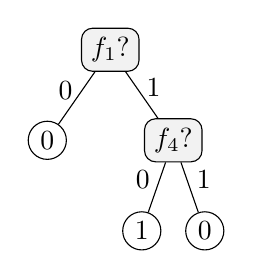
\begin{tikzpicture}[xscale=0.8,yscale=1.15]
    
    \tikzstyle{test} = [draw, rectangle, rounded corners, fill=
    gray!10]

    \tikzstyle{p} = [draw, circle, rounded corners, %fill= green!20,
    inner sep=2pt]

    \tikzstyle{n} = [draw, circle, rounded corners, %fill= red!20,
    inner sep=2pt]

    \draw
    (0,0) node [test] (A) {$f_1$?}
    (1,-1) node [test] (C) {$f_4$?}
    (-1,-1) node [n] (B) {0}
    (1.5,-2)  node [n] (E) {0}
    (0.5,-2)  node [p] (D) {1}
    ;

    \draw (A) -- (B) node [left,pos=0.35] {0};
     \draw (A) -- (C) node [right,pos=0.35] {1};
    \draw (C) -- (D) node [left,pos=0.35] {0};
     \draw (C) -- (E) node [right,pos=0.35] {1};
  \end{tikzpicture}
 \end{minipage}%
  \begin{minipage}{0.33\linewidth}
    \centering
  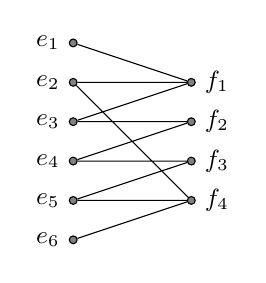
\begin{tikzpicture}[xscale=1.5,yscale=0.5]
    \small
    \tikzstyle{node} = [draw, circle, rounded corners, fill= gray,
    inner sep=1pt]

    \draw
    (0,0) node [node,label=left:$e_1$] (e1) {}
    (0,-1) node [node,label=left:$e_2$] (e2) {}
    (0,-2) node [node,label=left:$e_3$] (e3) {}
    (0,-3) node [node,label=left:$e_4$] (e4) {}
    (0,-4) node [node,label=left:$e_5$] (e5) {}
    (0,-5) node [node,label=left:$e_6$] (e6) {}

    (1,-1) node [node,label=right:$f_1$] (f1) {}
    (1,-2) node [node,label=right:$f_2$] (f2) {}
    (1,-3) node [node,label=right:$f_3$] (f3) {}
    (1,-4) node [node,label=right:$f_4$] (f4) {}

    (e2)--(f1)--(e3)--(f2)--(e4)--(f3)--(e5)--(f4)--(e2)
    (e1)--(f1)
    (e6)--(f4)
;

  \end{tikzpicture}
\end{minipage}%
 %  \begin{minipage}{0.3\linewidth}
%     \centering
%   \begin{tikzpicture}[xscale=1.5,yscale=0.5]
%     \small
%     \tikzstyle{node} = [draw, circle, rounded corners, fill= gray,
%     inner sep=1pt]

%     \draw
%     (0,0) node [node,label=left:$e_1$] (e1) {}
%     (0,-1) node [node,label=left:$e_2$] (e2) {}
%     (0,-2) node [node,label=left:$e_3$] (e3) {}
%     (0,-3) node [node,label=left:$e_4$] (e4) {}
%     (0,-4) node [node,label=left:$e_5$] (e5) {}
%     (0,-5) node [node,label=left:$e_6$] (e6) {}

%     (1,-1) node [node,label=right:$f_1$] (f1) {}
%     (1,-2) node [node,label=right:$f_2$] (f2) {}
%     (1,-3) node [node,label=right:$f_3$] (f3) {}
%     (1,-4) node [node,label=right:$f_4$] (f4) {}

%     (f1)--(e4) (f1)--(e5) (f1)--(e6)
%     (e3)--(f2)--(e4)
%     (f4)--(e1)
%     (f3)--(e2)
%     (f3)--(e3)
%     (f3)--(e6)
%     (e5)--(f4)--(e6) (e2)--(f4)
% ;

%   \end{tikzpicture}
% \end{minipage}%
 %   \begin{minipage}{0.3\linewidth}
 %    \centering
 %  \begin{tikzpicture}[xscale=0.8,yscale=1.15]
    
 %    \tikzstyle{test} = [draw, rectangle, rounded corners, fill=
 %    gray!10]

 %    \tikzstyle{p} = [draw, circle, rounded corners, %fill= green!20,
 %    inner sep=2pt]

 %    \tikzstyle{n} = [draw, circle, rounded corners, %fill= red!20,
 %    inner sep=2pt]

 %    \draw
 %    (0,0) node [test] (A) {$f_1$?}
 %    (-1,-1) node [test] (B) {$f_4$?}
 %    (1,-1) node [n] (C) {0}
 %    (-1.5,-2)  node [n] (D) {0}
 %    (-0.5,-2)  node [p] (E) {1}
 %    ;

 %    \draw (A) -- (B) node [left,pos=0.35] {0};
 %     \draw (A) -- (C) node [right,pos=0.35] {1};
 %    \draw (B) -- (D) node [left,pos=0.35] {0};
 %     \draw (B) -- (E) node [right,pos=0.35] {1};
 %  \end{tikzpicture}
 % \end{minipage}

\caption{%
  A CI $E=E^+\uplus E^-$ with six examples and four features (left), %
  a decision tree with~5 nodes that classifies $E$ (middle), %
  the incidence graph of the renaming $r_{\{f_2,f_4\}}(E)$,
  which has treewidth $2$ (right).} \label{fig:example}
\end{figure}


Key to our algorithm are new notions for succinctly representing
decision trees that correspond to subtrees of the incidence graph's
tree decomposition.  Based on that, we can carry out a dynamic
programming (DP) procedure along the tree decomposition.  However,
before we can apply the DP algorithm, we first need to find a renaming
of the given instance $E$ which minimizes the incidence graph's
treewidth. We achieve this by observing that the \emph{rank-width}
\cite{OumSeymour06} of $E$'s  incidence graph is linear in
its renamable treewidth. Thus, the rank-width is bounded by our
parameter (renamable treewidth), and so we can (i)~compute a rank
decomposition through a known fpt-algorithm~\cite{HlinenyOum08} and
(ii)~use a logical meta-theorem~\cite{DBLP:journals/dam/GanianH10} to
find a renaming $r_X(E)$ that minimizes the incidence treewidth.


While the DP approach using treewidth is quite well understood and can
often be quite easily designed for problems on graphs (or more
generally problems whose solutions can be represented in terms of the
graph for which the tree decomposition is given), the same DP approach
can become rather involved if applied to problems whose solutions have
no or only minor resemblence to the graph for which one is given a
tree decomposition. Probably the most prominent example for this is
the celebrated result by Bodlaender~\cite{Bodlaender96}, where he uses
a DP approach on an approximate tree decomposition to compute the
exact treewidth of a graph; here, the solutions are tree
decompositions, which are complex structures that cannot easily be
represented in terms of the graph. Other prominent examples include a
DP approach to compute the exact
treedepth~\cite{DBLP:conf/icalp/ReidlRVS14} or
clique-width~\cite{DBLP:journals/jgaa/EspelageGW03} using an optimal
tree decomposition.  We face a similar problem, since solutions in our
case are decision trees that do not bear any resemblence to the
incidence graph for which we are given the tree decomposition. The
main obstacle to overcome, therefore, is the design of the DP-records
for our DP algorithm. That is, a record for a node $b$ in a tree
decomposition for the incidence graph of $E$ needs to provide a
compact representation of partial solutions, i.e. partial solutions
in the sense that they represent the part of the solution for the
whole instance $E$ that corresponds to the sub-instance induced by all
features and examples contained in the bags in the subtree of the tree
decomposition rooted at the current node $b$. We overcome this
obstacle in Section~\ref{sec:twfpt}, where we also provide intuitive
descriptions and motivation for the definition of the records
(Subsection~\ref{ssec:mainideas}).

\ifshort
\emph{The full proof of statements marked with $(\star)$ can be found
  in the full version of this paper.}
\fi

\section{Preliminaries}\label{chap:prelims}

\subsection{Parameterized Complexity}
We give some basic definitions of Parameterized Complexity and refer
for a more in-depth treatment to other sources \cite{CyganFKLMPPS15,DowneyFellows13}.
Parameterized complexity considers problems in a two-dimensional
setting, where a problem instance is a pair $(I,k)$, where $I$ is the
main part and~$k$ is the parameter. A parameterized problem is
\emph{fixed-parameter tractable} if there exists a computable function
$f$ such that instances $(I,k)$ can be solved in time
$f(k) \|I\|^{O(1)}$.
% A parameterized problem is \emph{\XP-tractable}
% if instances $(I,k)$ can be solved in time $\|I\|^{f(k)}$. There are
% different shades of parameterized hardness. A problem is \paraNP-hard
% if fixing the parameter to a constant gives an NP-hard
% problem. Many parameterized problems that are \XP-tractable but not
% fixed-parameter tractable are contained in the complexity classes of
% the Weft hierarchy, $\W{1}\subseteq \W{2} \subseteq \dots$. Hardness
% for any of these classes provides a strong theoretical evidence for a
% problem to be not fixed-parameter tractable.
% For \DTL\ and \DTLh\ we consider mainly the three
% parameters solution size ($s$ for \DTL\ and $d$ for \DTLh), maximum
% domain size $D_{\max}$, and maximum difference $\delta_{\max}$.

\subsection{Graphs, Treewidth, and Rank-width}%\label{sec:graphs}

We will assume that the reader is familiar with basic graph theory 
(see, e.g. \cite{Diestel00,BangjensenGutin09}).  We
consider (vertex and edge labelled) undirected graphs. Let
$G=(V,E)$ be an undirected graph. We write $V(G)=V$ and $E(G)=E$ for
the sets of vertices and edges of $G$, respectively. We denote an edge
between $u \in V$ and $v \in V$ as $\{u,v\}$. For a set $V' \subseteq V$ of vertices
we let $G[V']$ denote the graph induced by the
vertices in $V'$, i.e. $G[V']$ has vertex set $V'$ and edge set $E \cap
\SB \{u,v\} \SM u,v \in V' \SE$ and we let $G - V'$ denote
the graph $G[V \setminus V']$. For a set $E' \subseteq E$ of edges we let denote
$G-E'$ the graph with vertex set $V$ and edge set $E\setminus E'$.
% We write
% $G=(V,E,\lambda)$ for a \emph{labeled graph} whose vertices and edges are
% labeled by a labeling function $\lambda$ where $\lambda$
% is a function from the vertices and edges of $G$ to some finite set of
% labels. 

%KD: New bit. Can surely be written better.
Node label control-width (NLC-width) is a graph parameter, defined as follows~\cite{Wanke94}:
Let $k \in \mathbb{N}$ be a positive integer.
A $k$-NLC-expression consists of a rooted subcubic tree such that:
\begin{enumerate}
\item Every leaf is labelled with a label $i \in \{1,\ldots,k\}$; this corresponds to a graph with a single vertex which has a label~$i$.
\item Every non-leaf node with one child is labelled with a function $R:\{1,\ldots,k\} \to \{1,\ldots,k\}$.
This corresponds to taking the labelled graph corresponding to the child and for every $i \in \{1,\ldots,k\}$, if a vertex has label~$i$, changing this label to be $R(i)$ instead.
\item Every non-leaf node with two children is labelled with a $k \times k$ $\{0,1\}$ matrix~$M$.
This corresponds to taking the disjoint union of the graphs corresponding to its children~$G_1$ and~$G_2$, and then for $i,j \in \{1,\ldots,k\}$, adding an edge from all vertices lablled~$i$ in~$G_1$ to all vertices labelled~$j$ in~$G_2$ if and only if $M_{i,j}=1$.
\item The root node corresponds to the resulting labelled graph.
\end{enumerate}
The NLC-width~$NLC(G)$ of a graph~$G$ is the minimum~$k$ for which~$G$ has a $k$-NLC-expression.
A $k$-NLC-expression is \emph{nice} if every relabelling node has a function $R:\{1,\ldots,k\} \to \{1,\ldots,k\}$ such that for some $i,j \in \{1,\ldots,k\}$, $R(i)=j$ and $R(\ell)=\ell$ for all $\ell \in \{1,\ldots,k\} \setminus \{i\}$.
%KD: Proably want to prove this (if we in fact need it) or give a reference.
Clearly, given a $k$-NLC-expression. a nice $k$-NLC-expression can be found in polynomial time.

Let~$x$ be a node in a $k$-NLC-expression tree of a graph~$G$.
We define~$\chi(X)$ to be the set of vertices in~$V(G)$ that correspond to leaves of the $k$-NLC-expression subtree rooted at~$x$.
%KD: Possibly wnat to prove this/provide a reference.
By the definifion of a $k$-NLC-expression, if $s,t \in \chi(X)$ have the same label after applying node~$x$ and $u \in V(G) \setminus \chi(X)$, then~$s$ is adjacent to~$u$ if and only if~$t$ is.
Furthermore, the $k$-NLC-expression subtree rooted at~$x$ is the graph induced by~$G$ on~$\chi(X)$.



%KD: TODO: Compare to clique-width/rank-width.
Computing the NLC-width of a graph is NP-hard~\cite{GW05}.


However, it is sufficient to use the algorithm of Seymour and Oum~\cite{OS06}, which returns a $c$-expression for some $c\leq 2^{3\cw(G)+2}-1$ in $O(n^9\log n)$ time, or the later improvements of Oum~\cite{Oum08} and Hlin\v{e}n\'y and Oum~\cite{HO08} that provide cubic-time algorithms which yield a $c$-expression for some $c\leq 8^{\cw(G)}-1$ and $c\leq 2^{\cw{G}+1}-1$, respectively.



%KD: Quoting: TODO: rephrase:
For example, although computing the clique-width of a graph is known to be \NP-hard in
general~\cite{FRRS09},\footnote{It is also \NP-hard to compute treewidth~\cite{ACP87} and parameters equivalent to clique-width, such as NLC-width~\cite{GW05}, rank-width (see~\cite{HO08,Oum08}) and boolean-width~\cite{SV16}.}
the complexity of computing the clique-width is open even on very restricted graph classes, such as unit interval graphs (see~\cite{HMR10} for some partial results).
As another example, the reason that rank-width and clique-width are equivalent is because the inequalities $\rw(G)\leq \cw(G)\leq 2^{\rw(G)+1}-1$ hold for every graph~$G$~\cite{OS06}.
Of course, this suggests we cannot hope to compute a $\cw(G)$-expression in polynomial time.
However, it is sufficient to use the algorithm of Seymour and Oum~\cite{OS06}, which returns a $c$-expression for some $c\leq 2^{3\cw(G)+2}-1$ in $O(n^9\log n)$ time, or the later improvements of Oum~\cite{Oum08} and Hlin\v{e}n\'y and Oum~\cite{HO08} that provide cubic-time algorithms which yield a $c$-expression for some $c\leq 8^{\cw(G)}-1$ and $c\leq 2^{\cw{G}+1}-1$, respectively.

%KD: End of new bit

%Treewidth is an important graph parameter that indicates in a certain sense
%the ``tree-likeness'' of a graph. 
%The \emph{treewidth} of an undirected graph $G=(V,E)$ is defined via the following
%notion of decomposition: a \emph{tree decomposition} of $G$ is a pair
%$(B,\chi)$ where $B$ is a tree and $\chi$ is a labelling function with
%$\chi(b)\subseteq V$ for every tree node $b$, such that the following
%conditions hold: 
%\begin{description}
%%\item Every vertex of $G$ occurs in $\chi(t)$ for some tree node~$t$.
%\item[(T1)] For every edge $\{u,v\}$ of $G$ there is a tree node $b$ such that $u,v\in \chi(b)$.
%\item[(T2)] For every vertex $v$ of $G$, the tree nodes $b$ with $v\in
%  \chi(b)$ induce a non-empty connected subtree of~$T$. 
%  % (``Connectednes Condition'').
%\end{description} 
%The \emph{width} of a tree decomposition $(B,\chi)$ is the size of a
%largest set $\chi(b)$ minus~$1$ among all nodes $b$ of~$B$.  A tree
%decomposition of smallest width is \emph{optimal}.  The \emph{treewidth}
%of a graph $G$, denoted $\tw(G)$, is the width of an optimal tree
%decomposition of~$G$.
%We let $B_b$ denote the subtree of $B$ rooted at a node $b$. 
%We use $\chi(B_b)$ to denote the set $\bigcup_{b'\in V(B_b)}\chi(b')$
%
%We simplify the presentation of our algorithm by using restricted tree
%decompositions. A tree decomposition is {\em nice} if
%\begin{itemize}
%\item[(1)] $\chi(r) = \emptyset$ for the root $r$ and $\chi(l)=\emptyset$
%  and for all leaf nodes $l$ in $B$, and
%\item[(2)]
%  every non-leaf node in $B$ is of one of the following types:
%  \begin{itemize}
%  \item An {\em introduce node}: a node $b$ with exactly one child $b_0$
%    such that $\chi(b) = \chi(b_0) \cup \{v\}$ for some $v \in V$.
%  \item A {\em forget node}: a node $b$ with exactly one child $b_0$
%    such that $\chi(b) = \chi(b_0) \setminus \{v\}$ for some $v \in V$.
%  \item A {\em join node}: a node $b$ with exactly two children $b_1$ and $b_2$
%    such that $\chi(b) = \chi(b_1) = \chi(b_2)$.
%  \end{itemize}
%\end{itemize}
%
%To make use of tree decomposition one first needs to be able to
%compute them.
%
%\begin{proposition}[{\cite{bodlaender1996efficient,Kl94}}]\label{pro:comp-ntd}
%  Let $G$ be a graph and $\omega \in \Nat$. We
%  can output a nice tree decomposition for $G$ of width at most
%  $\omega$ and size at most $\bigoh(\omega|V(G)|)$ or confirm
%  that the treewidth of $G$ is larger than $\omega$ in time $f(\omega)\cdot
%  n$, where $f$ is a computable function.
%\end{proposition}
%
% Given $G$ with $n$ vertices and a constant $w$, it is possible to decide
% whether $G$ has treewidth at most $w$, and if so, to compute an optimal
% tree decomposition of $G$ in time $O(n)$~\cite{Bodlaender96}.
% Furthermore there exist powerful heuristics to compute tree
% decomposition of small width in a practically feasible
% way~\cite{GogateDechter04}.

% We will now define rank-width that we will need to compute renamable
% treewidth. In order to define rank-width, we first need to define the
% \emph{cut-rank function} $\lambda_G$ that measures the complexity of a cut in
% an undirected graph $G$. For a subset $X$ of $V(G)$, we define
% $\lambda_G(X)$ as the rank of a $|X|\times |V(G)\setminus X|$ matrix
% $A_X$ over the binary field, where the entry of $A_X$ on the $i$-th
% row and the $j$-th column is $1$ if and only if the $i$-th vertex in
% $X$ is adjacent to the $j$-th vertex in $V(G)\setminus X$; if
% $X=\emptyset$ or $V(G)\setminus X=\emptyset$, then
% $\lambda_G(X)=0$.

% A tree is \emph{subcubic} if every node has degree $1$ or $3$. A
% \emph{rank-decomposition} of a graph $G$ is a pair $(T,\alpha)$, where
% $T$ is a subcubic tree with at least two nodes and $\alpha$ is a
% bijection from $V(G)$ to the set of all leaves of $T$. For each edge
% $e$ of $T$, $T-e$ induces a partition $(A_e,B_e)$ of the leaves of $T$
% and we say that the width of $e$ is equal to
% $\lambda_G(\alpha^{-1}(A_e))$; because $\lambda_G$ is symetric, it
% holds that the choice of $A_e$ over $B_e$ does not change the width of
% $e$. The \emph{width} of a rank-decomposition $(T,\alpha)$ is the
% maximum width of any of its edges. The \emph{rank-width} of a graph
% $G$, denoted by $\rw(G)$, is the minimum width over all
% rank-decompositions of $G$. If $G$ has less than two vertices, then
% $G$ has no rank-decomposition and we say that $G$ has rank-width $0$.

For our tractability result for renamable treewidth, we will also
require the notion of \emph{rank-width}, denoted by $\rw(G)$, which
like treewidth, is another important complexity measure for graphs. In
particular, we will need the following auxiliary results about rank-width.

\newcommand{\comp}[2]{\textup{comp}(#1,#2)}
\ifshort
Let $G$ be a bi-partite graph with partition $(A,B)$, i.e. $G$ is an
undirected graph and $G[A]$ and $G[B]$ are independent sets. For a set
$C \subseteq A\cup B$, we define the \emph{local bi-complement of $G$
  w.r.t. $C$} as the (bi-partite) graph $\comp{G}{C}$ with partition
$(A,B)$ having an edge between $a \in A$ and $b\in B$ if either
$\{a,b\}\setminus C\neq \emptyset$ and $\{a,b\} \in E(G)$ or
$\{a,b\} \subseteq C$ and $\{a,b\} \notin E(G)$.

\begin{proposition}[\cite{DBLP:journals/talg/Oum08,DBLP:journals/dam/KaminskiLM09,HlinenyOum08}]
  \label{pro:proprw}
  Let $G$ be a graph with $n\geq 2$ vertices, $S \subseteq V(G)$, and $\omega \in Nat$. Then:
  \begin{description}
  \item[(P1)] $\rw(G) \leq \tw(G)+1$,
  \item[(P2)] $\rw(\comp{G}{S})\leq 8\rw(G)$ (if $G$ is bi-partite) and
  \item[(P3)] We
    can output a rank-decomposition of width at most $\omega$ or confirm
    that the rank-width of $G$ is larger than $\omega$ in time $f(\omega)\cdot
    n^3$, where $f$ is a computable function.
  \end{description}
\end{proposition}
\fi

\iflong
\begin{proposition}[\cite{DBLP:journals/talg/Oum08}]\label{pro:rwtw}
  Let $G$ be a graph. Then, $\rw(G) \leq \tw(G)+1$.
\end{proposition}

%\newcommand{\comp}[2]{\textup{comp}(#1,#2)}
Let $G$ be a bi-partite graph with partition $(A,B)$, i.e. $G$ is an
undirected graph and $G[A]$ and $G[B]$ are independent sets. For a set
$C \subseteq A\cup B$, we define the \emph{local bi-complement of $G$
  w.r.t. $C$} as the (bi-partite) graph $\comp{G}{C}$ with partition
$(A,B)$ having an edge between $a \in A$ and $b\in B$ if either
$\{a,b\}\setminus C\neq \emptyset$ and $\{a,b\} \in E(G)$ or
$\{a,b\} \subseteq C$ and $\{a,b\} \notin E(G)$. We will need the
following proposition.

% rw+3;because one just adds three vertices and does local complements; can use the same refernece with some comment
\begin{proposition}[\cite{DBLP:journals/dam/KaminskiLM09}]\label{pro:rw-lcomp}
  Let $G$ be a bipartite graph and $S \subseteq V(G)$. Then,
  $\rw(\comp{G}{S})\leq 8\rw(G)$.
\end{proposition}
% \begin{proof}
  
%   \todo{todo}
%   % \begin{proposition}[{\cite[Proposition 6]{DBLP:journals/dam/KaminskiLM09}}]
% %   Local complementation does not change the rank-width of a graph.
% % \end{proposition}

% % \begin{proposition}[{\cite{DBLP:journals/dam/KaminskiLM09}}]
% %   Adding a vertex at most doubles the rank-width of a graph.
% % \end{proposition}

% % \begin{proposition}[{\cite{DBLP:journals/dam/KaminskiLM09}}]
% %   Removing a vertex does not increase the rank-width of a graph.
% % \end{proposition}

% % For complementing the edges between two disjoint subsets $U$ and $W$, we
% % introduce three new vertices $u$, $v$, and $w$ with $N(u)=U$, $N(v)=W$
% % and $N(w)=U\cup W$, apply local complementations centered at $u$, $v$
% % and $w$ and delete these three vertices. 

% % \begin{itemize}
% % \item from the above we obtain that $\rw(\GI(E)) \leq 6\rw(\GIL(E))$
% %   for any labeling.
% % \end{itemize}

% \end{proof}

\begin{proposition}[\cite{HlinenyOum08}]\label{pro:comprw}
  Let $\omega \in \Nat$ and $n\geq 2$. For an $n$-vertex graph $G$, we
  can output a rank-decomposition of width at most $\omega$ or confirm
  that the rank-width of $G$ is larger than $\omega$ in time $f(\omega)\cdot
  n^3$, where $f$ is a computable function.
\end{proposition}
\fi
%\subsection{MSO and a Meta-theorem for Rank-width}
%
%We consider \emph{Monadic Second Order} (MSO) logic on bi-partite
%graphs with partition $(A,B)$ in
%terms of their Gaifman structure whose universe contains vertices with
%two labels $A$ and~$B$ for the two parts of the bi-partition;
%the adjacency between vertices is represented by a
%binary relation $E$. We assume an infinite supply of \emph{individual
%  variables} $x,x_1,x_2,\dots$ and of \emph{set variables}
%$X,X_1,X_2,\ldots$. The \emph{atomic formulas} are $E xy$ (``vertex $x$
%is adjacent to vertex $y$''), $x=y$ (equality), $x\neq y$
%(inequality), $A x$ (``vertex $x$ is in $A$''), $B x$ (``vertex $x$ is
%in $B$''), and $X x$ (``vertex $x$ is an element of set $X$'').  \emph{MSO formulas} are built up
%from atomic formulas using the usual Boolean connectives
%$(\lnot,\land,\lor,\rightarrow,\leftrightarrow)$, quantification over
%individual variables ($\forall x$, $\exists x$), and quantification over
%set variables ($\forall X$, $\exists X$).
%
%Let $\Phi(X)$ be an MSO formula with a free set variable $X$. For a 
%graph $G=(V,E)$ and a set $S\subseteq V$ we write $G \models \Phi(S)$ if
%the formula $\Phi$ holds true on $G$ whenever $X$ is instantiated with~$S$.
%The following proposition shows that if $G$ has small rank-width then we
%can quickly check whether there is an $S$ with  $G \models \Phi(S)$.
%\begin{proposition}[{\cite[Theorem 4]{DBLP:journals/dam/GanianH10}}]\label{pro:courrw}
%  Let $\phi(X)$ be a MSO-formula. Given an $n$-vertex graph $G$,
%  we can decide whether there is a set $S\subseteq V(G)$ such that $G \models \phi(S)$ in time
%  $f(\rw(G)+|\phi|)\cdot n^3$, where $f$ is a computational function.
%  Moreover, if that is the case, then we can compute a set $S\subseteq V(G)$ with $G \models
%  \phi(S)$ in the same time.
%\end{proposition}
%% \ifshort
%% Note that strictly speaking~\cite[Theorem
%% 4]{DBLP:journals/dam/GanianH10} only states that given $S$ and $G$, we
%% can decide whether $G\models \phi(S)$ in the stated time. However, it
%% is easy to adapt their result to our setting (more details are in the
%% full version of this paper).
%% \fi
%\iflong
%However, 
%this also implies our proposition via self-reducibility. To see this,
%%KD: FIXME: This is double notation, since A is already defined above.
%consider the formula $\Phi(X)=\exists A (\forall a Xa \rightarrow Aa)
%\land \phi(X)$, then using~\cite[Theorem
%4]{DBLP:journals/dam/GanianH10} for $\Phi(X)$, we can check for every
%subset $S\subseteq V(G)$, whether $G\models \Phi(S)$. Moreover, we can
%use this to find a set $S$ with $G \models \phi(S)$ as follows. In the
%beginning, we set $S=\emptyset$. We then go over all vertices $v$ of
%$G$ and check whether $G\models \Phi(S\cup \{v\})$. If so we add $v$
%to $S$. Otherwise, we disregard $v$ and try the next vertex. Then, the
%set $S$ computed after trying all vertices of $G$ satisfies $G\models
%\phi(S)$, as required. Note that this algorithm is not optimal (since
%we get an additional factor of $n$ in the running time), we only use
%it here to illustrate that the result still holds. One can improve the
%run-time by adapting the proof of~\cite[Theorem
%4]{DBLP:journals/dam/GanianH10} to also work in our setting.
%\fi
%
%\ifshort
%\begin{lemma}[$\star$]
%\fi
%\iflong
%\begin{lemma}
%\fi  
%  \label{lem:twformula}
%  Let $\omega$ be an integer. Then, there is an MSO formula
%  $\Phi_\omega$ such that:
%  \begin{itemize}
%%KD: FIXME: remove pet hate ``it holds that''
%  \item For every graph $G$, it holds that $G \models \Phi_\omega$ if
%    and only if $G$ has treewidth at most $\omega$,
%  \item $\Phi_\omega$ can be computed in time $f(\omega)$ and
%    $|\Phi_\omega|\leq f(\omega)$ for some computable
%    function $f$.
%  \end{itemize}
%\end{lemma}
%\iflong
%\begin{proof}
%  We will construct $\Phi_\omega$ using the characterisation of graphs
%  of treewidth at most $\omega$ in terms of the excluded minors. We
%  first provide the necessary notions and definitions. A graph $H$ is
%  a \emph{minor} of a graph $G$ if $G$ has a \emph{minor model} $g$, i.e.
%  $g : V(H) \rightarrow 2^{V(G)}$ is a function such that:
%  \begin{itemize}
%  \item the sets $g(v)$ and $g(u)$ are disjoint for every distinct $v$
%    and $u$ in $V(H)$,
%  \item $G[g(v)]$ is connected for every $v \in V(H)$,
%  \item for every $\{u,v\} \in E(H)$, there is an edge in $G$ between
%    a vertex in $g(u)$ and a vertex in $g(v)$.
%  \end{itemize}
%  It follows from~\cite{DBLP:journals/jct/Lagergren98} that for every $\omega$ there is a family
%  $\mathcal{O}_\omega$ of graphs such that:
%  \begin{itemize}
%  \item a graph $G$ has treewidth at most $\omega$ if and only if
%    there is no graph $O \in \mathcal{O}_\omega$ such that $O$ is a minor of
%    $G$,
%  \item $\mathcal{O}_\omega$ can be constructed in time $f(\omega)$ and
%  \item the number and size of the graphs in $\mathcal{O}_\omega$ is bounded
%    by $f(\omega)$ for some computable function $f$.
%  \end{itemize}
%  Now, given $\mathcal{O}_\omega$, we can construct $\Phi_\omega$ as
%  the MSO formula such that $G \models \Phi_\omega$ if and only if $G$
%  does not contain any graph in $\mathcal{O}_\omega$ as a minor. It
%  therefore only remains to show that for a given $O\in
%  \mathcal{O}_\omega$, we can construct a formula $\Phi_0$ such that
%  $G \models \Phi_O$ if and only if $O$ is a minor of $G$. Using the
%  definition of a minor model from above, we can construct $\Phi_O$ as
%  follows (assuming that $V(O)=\{1,\dotsc,o\}$, where $o=|V(O)|$):
%  \[
%    \Phi_O = \exists V_1 \dotsb \exists V_{o}
%    (\bigwedge_{i=1}^{o}\textup{con}(V_i)) \land (\bigwedge_{1 \leq
%      i < j\leq o}\lnot \exists x V_ix \land V_jy) \land
%    (\bigwedge_{\{i,j\}\in E(O)}\exists x \exists y V_ix \land V_jy
%    \land Exy)
%  \]
%  where $\textup{con}(V_i)$ is the MSO formula that ensures that
%  $G[V_i]$ is connected and is defined by:
%%KD: FIXME: Double-notation again: A is already defined.
%  \[
%    \textup{con}(V_i)=\lnot (\exists A ((\forall a Aa \rightarrow V_i)
%    \land (\exists a \exists n A a \land \lnot A n \land V_i n)) \rightarrow (\exists a \exists n A a \land A n
%    \land V_i n \land Ean))
%  \]
%  Clearly, the length of $\Phi_O$ is bounded in terms of $|V(O)|$ and
%  since $|V(O)|$ and $|\mathcal{O}|$ are bounded in terms of $\omega$, 
%  the length of the complete formula $\Phi_\omega$ is bounded by a
%  function of $\omega$.
%\end{proof}
%\fi

\subsection{Classification Problems} An \emph{example} $e$ is a
function $e:\feat(e) \rightarrow \{0,1\}$ defined on a finite set
$\feat(e)$ of \emph{features}. For a set $E$ of examples, we put
$\feat(E)=\bigcup_{e\in E} \feat(e)$.  We say that two examples
$e_1,e_2$ \emph{agree} on a feature $f$ if $f \in \feat(e_1)$,
$f\in \feat(e_2)$ and $e_1(f)=e_2(f)$. If $f \in \feat(e_1)$,
$f \in \feat(e_2)$ but $e_1(f)\neq e_2(f)$, we say that the examples
\emph{disagree on $f$}.


A \emph{classification instance (CI)} (also called a \emph{partially defined
Boolean function}\ \cite{IbarakiCramaHammer11})
$E=E^+ \uplus E^-$ is the disjoint union of two sets of examples, where
for all $e_1,e_2\in E$ we have $\feat(e_1)=\feat(e_2)$. The examples
in $E^+$ are said to be \emph{positive}; the examples in $E^-$ are said to be
\emph{negative}.  A set $X$ of examples is \emph{uniform} if
$X\subseteq E^+$ or $X \subseteq E^-$; otherwise $X$ is \emph{non-uniform}.
 
Given a CI $E$, a subset $F\subseteq \feat(E)$ is a \emph{support set}
of $E$ if any two examples $e_1\in E^+$ and $e_2\in E^-$ disagree in
at least one feature of $F$.  Finding a smallest support set, denoted
by $\MSS(E)$, for a classification instance $E$ is an NP-hard
task~\cite[Theorem 12.2]{IbarakiCramaHammer11}.

% For two examples $e$ and $e'$ in $E$, we denote by $\HD(e,e')$ the
% set of features where $e$ and $e'$ disagree and we denote by
% $\MHD(E)=\max_{e^+\in E^+ \land e^- \in E^-}\Card{\HD(e^+,e^-)}$ the
% \emph{maximum difference} between any two non-uniform examples.
% For a feature $f \in \feat(E)$, we denote by $D_E(f)$ the set of
% domain values for $f$ appearing in any example of $E$, i.e. $D_E(f)=\SB e(f)
% \SM e \in E \SE$ and we set $\DMAX$ to be the maximum size of $D_E(f)$
% over all features of $E$, i.e. $\DMAX=\max_{f \in \feat(E)}\Card{D_E(f)}$.
% A CI is called \emph{Boolean}\footnote{Boolean classification instances are also called \emph{partially defined
%   Boolean functions} \cite{IbarakiCramaHammer11}.} if $\DMAX=2$.
% We denote by $E[\alpha]$ the set of examples in $E$ that agree with
% the assignment $\alpha : F' \rightarrow \{0,1\}$, where $F' \subseteq
% \feat(E)$, i.e. $E[\alpha]=\SB e \SM e(f)=\alpha(f) \land f \in
% F'\SE$.
% % Similarly, if $\alpha : F' \rightarrow \IV(\GD)$ assigns
% % every feature in $F'$ an interval from the set $\IV(\GD)$ of all
% % open, half-open, and closed intervals over~$\GD$, then
% % $E[\alpha]=\SB e \SM e(f)\in \alpha(f) \land f \in F'\SE$.
% For the complexity analysis we set the \emph{input size} $\|E\|$ of a
% CI  $E$ to $\Card{E}
% \cdot (\Card{\feat(E)}+1) \cdot \log D_{\max}$.
 
We define the \emph{incidence graph} of $E$, denoted by $\GI(E)$, as
the bipartite graph with partition $(E, \feat(E))$ having an edge
between an example $e \in E$ and a feature $f\in \feat(e)$ if
$f(e)=1$.

Finally, we define a
\emph{renaming} $r_X(E)$ of a CI $E$ with respect to a set 
$X\subseteq F(E)$ to be the CI containing all the examples $e_X$ for
$e\in E$ with $e_X(f)=1-e(f)$ if $f\in X$ and $e_X(f)=e(f)$ if
$f\notin X$.

% We say that $E|S$ is obtained by \emph{renaming the features in $S$}.
\ifshort
\begin{observation}[$\star$]
\fi
\iflong
\begin{observation}
\fi  
  \label{obs:rename}
  Let $E$ be a CI and $X \subseteq \feat(E)$. Then, $E$ has a DT of
  size $s$ if and only if $r_X(E)$ does.
\end{observation}
\iflong
\begin{proof}
  Let $T$ be a DT for $E$ and let $T'$ be obtained from $T$ by switching
  the left and right child of every node $t$ of $T$ with $\feat(t)\in
  X$. Then $T'$ is DT for $r_X(E)$ having the same size as $T$.
\end{proof}
\fi

\subsection{Decision Trees}

A \emph{decision tree} (DT) (or
\emph{classification tree}) is a rooted tree $T$ with vertex set
$V(T)$ and arc set $A(T)$, where each non-leaf node (called a
\emph{test}) $v\in V(T)$ is labelled with a feature $\feat(v)$, each
non-leaf node $v$ has exactly two out-going arcs, a \emph{left arc}
and a \emph{right arc}, and each leaf is either a \emph{positive} or a
\emph{negative} leaf. We write
$\feat(T)=\SB v\in V(T) \SM \feat(v) \SE$.
%
% Given a CI $E=E^+\uplus E^-$, and a decision tree
% $T$ with $\var(T)\subseteq \var(E)$, there is a unique leaf of $T$,
% denoted $\leaf_T(E)$, such that all the examples literals appearing in labels
% along the unique path from the root to $t$ belong to~$\leaf_T(S)$.

Consider a CI $E$ and a decision tree $T$ with
$\feat(T)\subseteq \feat(E)$. For each node $v$ of $T$ we define
$E_T(v)$ as the set of all examples $e\in E$ such that for each left
(right, respectively) arc $(u,v)$ on the unique path from the root of
$T$ to~$v$ we have $e(\feat(v))=0$
($e(\feat(v))=1$, respectively).  $T$ \emph{correctly
  classifies} an example $e\in E$ if $e$ is a positive (negative)
example and $e\in E_T(v)$ for a positive (negative) leaf. We say that $T$
\emph{classifies} $E$ (or simply that $T$ is a DT for $E$)
if $T$ correctly classifies every example $e \in E$. See
Figure~\ref{fig:example} for an illustration of a CI, its incidence
graph, and a DT that classifies $E$.
% An example for a
% CI $E$ and a possible DT for $E$ are
% illustrated in Figure~\ref{fig:walk}.
% The \emph{depth} $d(T)$ of a DT $T$ is the length of a
% longest path from the root to a leaf and the \emph{size} $|T|$ of $T$
% is equal to $|V(T)|$. 
% The \emph{size} of $T$, denoted by $|T|$, is the number of non-leaf
% nodes (tests) in $T$ and the \emph{depth} of $T$, denoted by
% $\dep(T)$, is the maximum number of non-leaf nodes (tests) in any
% root-to-leaf path of $T$.  \ifshort \DTL{} (and \DTLh{}) are now the
% problems of deciding whether for a given CI $E$ and an integer $s$
% ($d$), there is a DT for $E$ of size at most $s$ (depth at most $d$).
% \fi
% \begin{observation}\label{obs:dt-ss}
%   Let $T$ be a DT for a CI $E$, then
%   $\feat(T)$ is a support set of $E$.
% \end{observation}
% \begin{proof}
%   Suppose for a contradiction that this is not the case and there is
%   an example $e^+ \in E^+$ and an example $e^- \in E^-$
%   such that $e^+$ and $e^-$ agree on all features in
%   $\feat(T)$. Therefore, $e^+$ and $e^-$ are contained in the same leaf
%   node of~$T$, contradicting our assumption that $T$ is a DT.
% \end{proof}
The size of $T$ is its number of nodes, i.e. $|V(T)|$.
\iflong We consider the following problem.
\pbDef{\probfont{Minimum Decision Tree Size} (\DTL)}{A classification
  instance $E$ and an integer $s$.}{Is there a decision
  tree of size at most $s$ for $E$?}
\fi
We now give some simple auxiliary lemmas that are required by our
algorithm.
\ifshort
\begin{lemma}[$\star$]
\fi
\iflong
\begin{lemma}
\fi
  \label{lem:enum-dt-fund}
  Let $A$ be a set of features of size $a$. Then the number of DTs of
  size at most $s$ that use only features in $A$ is at most
  $a^{2s+1}$ and those can be enumerated in $\bigoh(a^{2s+1})$ time.
\end{lemma}
\iflong
\begin{proof}
  We start by counting the number of
  trees $T$ with $n$ nodes that can potentially underlie a DT with $n$ nodes. Note that
  there is one-to-one correspondence between 
  trees $T$ that underlie a DT with $n$ nodes and unlabelled rooted ordered binary trees with
  $n$ nodes (where ordered refers to an ordering of the at most $2$
  child nodes). Since it is known
  that the number of unlabelled rooted ordered binary trees with $n$
  nodes is equal to the $n$-th Catalan number $C_n$ and that those
  trees can be
  enumerated in $\bigoh(C_n)$ time~\cite{stanley2015catalan}, we already obtain that we
  can enumerate all of the at most $C_n$ possible trees $T$ underlying
  a DT of size $n$ in $\bigoh(C_n)$ time.
  Therefore, there are at most
  $sC_{s}$ possible trees of size at most $s$ that can underlie a
  DT with at most $s$ nodes and those can be enumerated in
  $\bigoh(sC_{s})$ time. It now remains to bound the number of possible
  feature assignments $\feat(f)$ for these trees as well as the number
  of possibilities for the leave nodes that can be either labelled
  positive or negative. Since we can assume that $a\geq 2$, we obtain
  that the number of possible feature assignments (and labellings of
  leaf-nodes) of a tree $T$ with $n$ nodes is at most $a^n$. Taking
  everything together, we obtain that there are at most
  $sC_sa^s \leq s4^sa^s \leq a^{2s+1}$ many
  DTs of size at most $s$ using only
  features in $A$ and those can be enumerated in $\bigoh(a^{2s+1})$ time.
\end{proof}
\fi

\ifshort
\begin{lemma}[$\star$]
\fi
\iflong
\begin{lemma}
\fi
  \label{lem:enum-dt}
  Let $A$ be a set of features of size $a$. There are at most
  $a^{2^{a+1}+3}$ inclusion-wise minimal DTs using only features in
  $A$ and these can be enumerated in $\bigoh(a^{2^{a+1}+3})$ time.
\end{lemma}
\iflong
\begin{proof}
  Note that an inclusion-wise minimal DT $T$ that uses only features in
  $A$ has at most $2^a+1$ nodes; this is because every feature appears
  at most once on every path $T$. Therefore, we obtain from Lemma~\ref{lem:enum-dt-fund}
  that the number of choices for $T$ is at most $a^{2(2^a+1)+1}=a^{2^{a+1}+3}$
\end{proof}
\fi

\newcommand{\NO}{\textbf{NO}}

\newcommand{\TsmDT}{(2^{|E|})^{4|E|-1}}
\ifshort
\begin{lemma}[$\star$]
\fi
\iflong
\begin{lemma}
\fi
\label{lem:comsmallDT}
  Let $E$ be a CI. Then one can decide whether $E$ has a DT and if so
  output a DT of minimum size for $E$ in time $\bigoh(\TsmDT)$.
\end{lemma}
\iflong
\begin{proof}
  Note first that $|\feat(E)|\leq 2^{|E|}$ since we can assume that
  $E$ does not contain two equivalent features. Moreover, $E$ has a DT if
  and only if $\feat(E)$ is a support set, which can be checked in
  time $\bigoh(|E|^2|\feat(E)|)$ by checking, for every pair of
  positive and negative examples in $E$, whether there is a feature that
  distinguishes them. If this is not the case, we output
  \NO{}, so assume that $E$ has a DT. Note that any inclusion-wise
  minimal DT for $E$ has at most $|E|$ leaves and therefore size at most
  $2|E|-1$. We can therefore employ Lemma~\ref{lem:enum-dt-fund} to
  enumerate all inclusion-wise minimal potential DTs for $E$ in time
  $\bigoh((2^{|E|})^{2(2|E|-1)+1}) \in \bigoh(\TsmDT)$. For every such
  tree we then check whether it is
  indeed a DT for $E$ and return a DT for $E$ of minimum size found
  during this process.
\end{proof}
\fi

\section{Introducing and Computing Renamable Treewidth}

In this section, we are introducing our novel parameter called
renamable treewidth. Let $E$ be a CI. Then we could define the
treewidth of $E$ as the treewidth of the incidence graph
$\GI(E)$. However, since $\GI(E)$ has an edge between every example $e
\in E$ and feature $f \in \feat(E)$ such that $e(f)=1$, the treewidth
of $\GI(E)$ depends very much on the concrete values that the examples
take for different features. For instance, consider the CI $E$ with $n$
examples $e_1,\dotsc,e_n$ and $n$ features $f_1,\dotsc,f_n$ such that
$e_i(f_j)=0$ if and only if $i=j$, i.e. the matrix with features and
examples is the complement of the identity matrix. Then
the $\GI(E)$ is a bi-clique minus a perfect matching and therefore its treewidth is arbitrary
large (i.e. to be exact it is easy to verify that its treewidth is $n-1$). However, if we rename the values of all
features, i.e. if we consider the CI $r_{\feat(E)}(E)$, then its treewidth
is $1$ (since $\GI(r_{\feat(E)}(E))$ is a perfect matching)
even though $E$ and $r_{\feat(E)}(E)$ lead to equivalent instances of
\DTL{} (Observation~\ref{obs:rename}). Therefore, it would be much
better to consider the minimum treewidth of $\GI(r_X(E))$ over every
possible choice for $X \subseteq \feat(E)$. This leads us directly to
our new notion \emph{renamable treewidth} of a CI~$E$, denoted by
$\rtw(E)$, which we define as $\rtw(E)=\min_{X\subseteq
  \feat(E)}\tw(\GI(r_X(E)))$.

Unfortunately, unlike treewidth, where it is known that an optimal
tree decomposition can be computed in fpt-time, this is not known for
renamable treewidth. However, it is required for our algorithm to
work. The remainder of this section is therefore devoted to a proof of
the following theorem.

\begin{theorem}\label{the:comprtw}
  Let $E$ be a CI and $\omega$ and integer. Then, there is an
  algorithm that in time $o(\omega)\cdot n^3$ decides whether $\rtw(E)\leq
  \omega$ and if so computes a subset $X \subseteq \feat(E)$ such that
  $\tw(\GI(r_X(E)))\leq \omega$, for some computable function $o$.
\end{theorem}
\begin{proof}
  We start by showing that $\rw(\GI(E)) \leq 8\rtw(E)+1$. Let $X
  \subseteq \feat(E)$ such that $\tw(\GI(r_X(E)))=\rtw(E)$. Then,
  $\GI(r_X(E))$ is the local bi-complement of $\GI(E)$ w.r.t. the
  set $C=X\cup E$. Therefore, we obtain from \iflong
  Proposition~\ref{pro:rw-lcomp}\fi\ \ifshort
  Proposition~\ref{pro:proprw} (P2)\fi\ that $\rw(\GI(E))\leq 8\rw(\GI(r_X(E)))$, which because of
  \iflong Proposition~\ref{pro:rwtw}\fi\ \ifshort
  Proposition~\ref{pro:proprw} (P1)\fi\  implies that $\rw(\GI(E)) \leq 8\rtw(E)+1$, as
  required.

  To compute $X$, we will make use of
  Proposition~\ref{pro:courrw}. That is, we will construct an MSO
  formula $\phi(X)$ such that:
  \begin{description}
  \item[(C1)] $\GI(E) \models \phi(X)$ if and only if $X$ is a set of
    features of $E$ such that $\tw(\GI(r_X(E))) \leq \omega$,
%  \item[(C2)] $|\phi(X)|\leq g(\omega)$ for some computable function $g$,
  \item[(C2)] $\phi(X)$ can be constructed in time $g(\omega)$ and
    $|\phi(X)|\leq g(\omega)$ for some
    computable function~$g$.
  \end{description}
  Once we have $\phi(X)$, we can compute $X$ as follows:
  \begin{itemize}
  \item First we use \iflong Proposition~\ref{pro:comprw}\fi\ \ifshort Proposition~\ref{pro:proprw} (P3)\fi\ to decide in time
    $f(\rw(\GI(E)))\leq f(8\omega+1)\cdot n^3$ whether
    $\rw(\GI(E))\leq 8\omega+1$. If this is not the case, then we know
    that $\rtw(E)>\omega$ and we can reject.
  \item Otherwise, we construct the MSO formula $\phi(X)$ in time
    $g(\omega)$ and use Proposition~\ref{pro:courrw} to decide in time
    $f(\rw(\GI(E))+g(\omega)) \cdot n^3\leq f(8\omega+1+g(\omega))
    \cdot n^3$ whether
    there is a set $X$ such that $\tw(\GI(r_X(E))) \leq \omega$. If
    that is the case we return $X$ and if not we correctly reject.
  \end{itemize}
  Therefore, it only remains to show how to construct $\phi(X)$.
  Let $\Phi_\omega$ be the MSO formula given by
  Lemma~\ref{lem:twformula}. Moreover, let $\Phi_\omega'$ be the MSO
  formula obtained from $\Phi_\omega$ after replacing every occurrence
  of an atomic formula $Exy$ with the formula $\phi_E(x,y)$ given by:
  \[
    (\lnot X x \land \lnot
  X y \rightarrow Exy)\land ((Xx \lor Xy) \land (\lnot A x \lor \lnot
  Ay) \rightarrow \lnot Exy) \land ((Ax \land Ay)\rightarrow \lnot
  Ax);
  \]
  here $Ax$ is true if $x$ is a feature vertex of $\GI(E)$.
  Note that the formula $\phi_E(x,y)$ is true if and only if $x$ is adjacent to
  $y$ in $\GI(r_X(E))$. Then, $\phi(X)$ is the formula $\exists X
  (\forall x Xx \rightarrow Ax) \land \Phi_\omega'$. It is
  straightforward to verify that $\phi(X)$ satisfies (C1)--(C2).
\end{proof}

% \begin{lemma}
%   \begin{itemize}
%   \item $\rw(G) \leq \tw(G)+1$~\cite{DBLP:journals/talg/Oum08}
%   \item $\rw(\GI(E)) \leq 8\rw(\GI(E_\lambda))$ for every relabel
%     function $\lambda : \feat(E) \rightarrow \{0,1\}$,
%   \item for every $\omega$ a MSO$_1$-formula $\phi_\omega$ with
%     $|\phi_\omega|\leq ?$ can be constructed in time $\bigoh(?)$ such
%     that $G \models \phi_\omega$ if and only if $G$ has treewidth at
%     most $\omega$ (maybe from the references in the soda paper?)
%   \end{itemize}
% \end{lemma}



\newcommand{\exam}{\text{\specialfont{exam}}}

\section{An FPT-Algorithm for NLC-width}

\label{sec:twfpt}
\newcommand{\afs}{\textup{TF}}
\newcommand{\afsF}{\textup{TF}_F}
\newcommand{\afsP}{\textup{TF}_P}
\newcommand{\addF}{\oplus}

In this section, we present our main result, i.e. we will show
that \DTL{} is fixed-parameter tractable parameterized by 
NLC-width.
\begin{theorem}\label{the:trac-tw-b}
  \DTL{} is fixed-parameter tractable parameterized by NLC-width.
\end{theorem}
%Given a CI $E$, our algorithm starts by using
%Theorem~\ref{the:comprtw} to compute a set $X$ such that
%$\tw(\GI(r_X(E)))=\rtw(E)$. It then replaces $E$ with $r_X(E)$ and
%uses Proposition~\ref{pro:comp-ntd} to compute a nice tree
%decomposition of $\GI(E)$ whose width $\omega$ is equal to
%$\rtw(E)$. Therefore, to complete the proof of Theorem~\ref{the:trac-tw-b}, it
%suffices to show the following.
%KD: TODO: Add some text about computing an approximate NLC-width decomposition.
\begin{theorem}\label{the:trac-nlcw-b-td}
  Let $E$ be a CI, let $(T,\chi)$ be an NLC-expression decomposition of
  width $k$ for $\GI(E)$, and let $s$ be an integer. Then,
  deciding whether $E$ has a DT
  of size at most $s$ is
  fixed-parameter tractable parameterized by $k$.
\end{theorem}

%KD: Some edits in the following paragraph, but not quite right yet.
In principle, we will use a dynamic programming algorithm along the NLC-expression $(T,\chi)$ of $\GI(E)$ that computes a set of records for every node $b$ of $B$ in a bottom-up manner.
Each record will represent an equivalence class of solutions (DTs) for the whole instance restricted to the examples and features represented by the current subtree rooted in $b$, i.e. the examples and features contained in $\chi(B_b)$.
Before we continue with the formal notions and definitions required to define the records, we want to illustrate the main ideas and motivations.
In what follows let $(B,\chi)$ be an NLC-width expression of
%KD: Why the +1?
$\GI(E)$ for the CI $E$ of width $k$. For $b \in V(B)$, we write $\feat(b)$ and $\exam(b)$ for the sets $\chi(b)\cap\feat(E)$ and $\chi(b)\cap E$, respectively.
Similarly, we write $\feat(B_b)$ and $\exam(B_b)$ for the sets $\chi(B_b)\cap\feat(E)$ and $\chi(B_b)\cap E$, respectively.

\subsection{Description of the Main Ideas Behind the Algorithm}
\label{ssec:mainideas}
Consider a node $b$ of $B$. To simplify the presentation, we will
sometime refer to the features and examples in $\chi(B_b)\setminus
\chi(b)$ as \emph{forgotten} features and examples and we refer to the
features and examples in $(\feat(E)\cup E)\setminus \chi(B_b)$ as
\emph{future} features and examples. We start with some simple observations that follow
immediately from the properties of tree decompositions.

\begin{observation}\label{obs:td-prop-exfe}
  \begin{itemize}
  \item[(1)] $e(f)=0$ for every forgotten example $e \in \exam(B_b)\setminus
    \exam(b)$ and future feature $f \in \feat(E)\setminus \feat(B_b)$,
  \item[(2)] $e(f)=0$ for every future example $e \in E\setminus
    \exam(B_b)$ and forgotten feature $f \in \feat(B_b)\setminus \feat(b)$;
  \end{itemize}
\end{observation}
\begin{proof}
  Towards showing (1), let $e$ be an example in $\exam(B_b)\setminus
  \exam(b)$ and let $f$ be a feature in $\feat(E)\setminus
  \feat(B_b)$. We claim that because $(T,\chi)$ is a tree
  decomposition of $\GI(E)$, the graph $\GI(E)$ cannot contain an edge
  between $e$ and $f$, which implies that $e(f)=0$. Suppose for a
  contradiction that this is not the case, i.e. $\{e,f\} \in
  E(\GI(E))$. Then, because of property (T1) of a tree decomposition,
  there must exist a node $b'$ such that $e,f\in \chi(b')$. But then,
  if $b' \in V(B_b)$ we obtain that $f \notin \chi(b')$. Similarly, if
  $b' \in V(B\setminus B_b)$, we obtain that $e \notin \chi(b')$ since
  otherwise $e$ would violate property (T2) of a tree
  decomposition. This completes the proof for (1); the proof for (2)
  is analogous.
\end{proof}
Informally, Observation~\ref{obs:td-prop-exfe} shows that forgotten
examples cannot be distinguished by future features and future
examples cannot be distinguished by forgotten features. 

Consider a DT $T$ for $E$ and a node $b$ of $B$. For a set $W$
containing features and examples from $E$, we denote by
$E[W]$ the sub-instance of $E$ induced by the features and examples in
$W$. Our aim is to obtain
a compact representation (represented by records) of the partial solution for the sub-instance
$E[\chi(B_b)]$ of $E$ induced by the features and examples in
$\chi(B_b)$ represented by $T$.

Intuitively, such a compact representation
has to (1) represent a partial solution (DT) for the examples in $\exam(B_b)$ and (2)
retain sufficient information about the structure of $T$ in order to
decide whether it can be extended to a DT that also classifies the
examples in $E\setminus \exam(B_b)$. 

For illustration purposes let us first consider the simplified case
that $\exam(b)=\emptyset$. Because of
Observation~\ref{obs:td-prop-exfe} (1), this implies that every forgotten
example goes to the left child of any node $t$ in $T$ that is assigned
a future feature. Therefore, under the assumption that
$\exam(b)=\emptyset$ the DT $T'$ obtained from  $T$ after:
\begin{itemize}
\item removing the subtree $T_r$ of $T$ for every right child $r$ of a
  node $t$ of $T$ with $\feat(t) \in \feat(E)\setminus \feat(B_b)$ and
  replacing $t$ with an edge from its parent in $T$ to its left child
  in $T$
\end{itemize}
is a DT for $E[\chi(B_b)]$. Note that this means that under the rather
strong assumption that $\exam(b)=\emptyset$, the part of $T$ that
takes care of the sub-instance $E[\chi(B_b)]$ is itself a DT using
only features in $\feat(B_b)$; we will see later that unfortunately
this is no longer the case if $\exam(b)\neq \emptyset$. Note that even
though $T'$ is a DT for $E[B_b]$, it does not yet constitute a
compact representation, since the number of features it uses in
$\feat(B_b)\setminus \feat(b)$ is potentially unbounded. However, we
obtain from Observation~\ref{obs:td-prop-exfe} (2) that every future
example will end up in the left child of every node $t$ of $T'$ that
is assigned a forgotten feature. This means that to decide whether
$T'$ can be extended to a DT for the whole instance, the nodes that are
assigned forgotten features are not important. In fact, the only nodes
in $T'$ that can be important for the classification of future
examples are the nodes that are assigned features in
$\feat(b)$. That is, it is sufficient to
remember the DT $T''$ obtained from $T'$ after:
\begin{itemize}
\item removing the subtree $T_r$ of $T'$ for every right child $r$ of a
  node $t$ of $T'$ with $\feat(t) \in \feat(B_b)\setminus \feat(b)$ and
  replacing $t$ with an edge from its parent in $T'$ to its left child
  in $T'$
\end{itemize}
Since the number of possible DT $T''$ is clearly bounded in terms of
the number of features in $\feat(b)$ (and therefore in terms of the
treewidth of $\GI(E)$), this would already give us the compact
representation that we are looking for. However, this only works in the case
that $\exam(b)=\emptyset$, which is clearly not the case in general.

So let us now consider the general case with $\exam(b)\neq
\emptyset$. The first difference now is that the part of $T$ that
takes care of the sub-instance $E[\chi(B_b)]$ is no longer a DT that
only uses features in $\feat(B_b)$. In fact, it could even be the case
that $E[\chi(B_b)]$ does not have a DT, because there could exist
examples in $\exam(b)$ that can only be distinguished using the
features in $\feat(E)\setminus \feat(B_b)$. This means that we have to
allow our partial solution for $E[\chi(B_b)]$ to use future
features. Fortunately, we do not need to know which exact future
feature is used by our partial solution but it suffices to know
that a future feature is used and how it behaves w.r.t. the examples
in $\exam(b)$; this is because Observation~\ref{obs:td-prop-exfe} (1)
implies that a future feature is used in a partial
solution only for the purpose of distinguishing examples in
$\exam(b)$. Moreover, because every forgotten example ends up in the
left child of any node $t$ of $T$ that uses a future feature, we only
need to remember the left child for those nodes. Also, we only need to
remember occurrences of those nodes (using future features) if at least
one example in $\exam(b)$ ends up to in the right child of such a
node; otherwise the node has no influence on the classification of
examples in $\exam(B_b)$. Finally, we cannot simply forget nodes that use
forgotten features (as we could in the case that $\exam(b)=0$). This
is because we need to know exactly where the examples in $\exam(b)$
end up at. For instance, if such an example in $\exam(b)$ ends up in the
right child of a node using a future feature, we need to know that
this is the case because this means that the example has to be
classified in this place at a later stage of the
algorithm. Nevertheless, we do not need to remember all occurrences of
nodes using forgotten features, but only those for which there is at
least one example in $\exam(b)$ that ends up in the right child of the
node. Similarly, we do not need to remember the exact forgotten
feature that is used but only how it behaves towards the examples in
$\exam(b)$. In summary, we only need to remember the full information
about the nodes of $T$ that use a feature in $\feat(b)$. For all other
nodes, i.e. nodes that use either forgotten or future features, we only
need to remember such a node, if at least one example in $\exam(b)$ ends up in
its right child. Moreover, even if this is the case, we only need to
remember the following for such nodes:
\begin{itemize}
\item whether it uses a future or a forgotten feature and
\item how it behaves w.r.t. the examples in $\exam(b)$.
\end{itemize}

With these ideas in mind, we are now ready to provide a formal
definition of the compact representation of the part of $T$ that
takes care of the sub-instance $E[\chi(B_b)]$.

\subsection{Formal Definition of Records and Preliminary Results}

Consider a node $b \in V(B)$.
We start by introducing novel features that will model the behaviour of future features on the examples in $\exam(b)$.
For a subset of labels $B \in \{1,\ldots,k\}$, we define the feature template $f_B$ by setting $e(f_B)=1$ if and only if $lab(e) \in B$ and $e(f_B)=0$ otherwise.


Notes: In our DT, we have leaves labelled $+$ or $-$.
We have can have actual features with labels in $\{1,\ldots,k\}$ (because of the NLC-expression, we can choose any representative, and it will work the same as everything else).
We can also have feature templates: there are at most~$2^k$ of these, depending on whether they will send each label in $\{1,\ldots,k\}$ to the right or to the left.
Note: whenever we have a relabelling node, these templates will need to be mangled.
Note: when we do a join node, we need to check which label actual features actually exist in each subtree.

Reduction algorithm:
Notation: for $X \in \{1,\ldots,k\}$, let $\overline{X}=\{1,\ldots,k\} \setminus X$.

Suppose we have a DT such that some actual feature~$f$ occurs twice on a path from the root to the leaves, say~$f_1$ is the instance closer to the root and~$f_2$ is the other instance.
If~$f_2$ is in the left (resp. right) subtree of~$f_1$, we delete $f_2$'s right (resp. left) subtree.
We then contract away the node~$f_2$ (i.e. replace the subtree rooted at~$f_2$ by the subtree rooted at $f_2$'s unique remaining child.
Now suppose we have a feature template~$B$ in our decision tree.
Let $B_1,\ldots,B_\ell$ be the sequence of feature templates on the path from the root to~$B$ in order (not including~$B$, so~$B_\ell$).
Let $B_i'=B_i$ if~$B$ is in the right sub-tree of~$B_i$ and let $B_i'=\overline{B_i}$ otherwise.
If $\overline{B} \subseteq B_1' \cup \cdots \cup B_\ell'$, then we delete the subtree rooted at the left child of~$B$ and contract~$B$ away.
If $B \subseteq \overline{B_1'} \cup \cdots \cup \overline{B_\ell'}$, then we delete the subtree rooted at the right child of~$B$ and contract~$B$ away.
If this procedure has been applied to a record exhaustively, we say that the record is \emph{reduced}.

The \emph{score} of a record at a node~$x$ is the number of actual features used in the DT for the nodes in~$\chi(x)$ (disregarding any feature templates).
A record is \emph{complete} if it contains no feature templates.

\begin{lemma}\label{lem:reduced-tree-height}
If there are~$k$ actual feature labels and~$\ell$ future templates labels, then every reduced DT has height at most $k+\ell$.
Futhermore, every path from the root to the leaves contains at most~$k$ actual feature labels and at most $\ell-1$ future templates.
\end{lemma}

\begin{proof}
Consider a path~$P$ of maximum length from the root to the leaves in a reduced DT.
No actual feature appears more than once on this path, so the number of actual feature nodes on this path is at most~$k$.
%KD: TODO: This needs to be explained properly.
Each feature template must divide the set of colours into two non-empty parts, so there can be at most $\ell-1$ feature template nodes on this path.
The path ends with a leaf node, so this gives a total of $k+\ell-1+1=k+\ell$ nodes, as required.
\end{proof}

\begin{lemma}\label{lem:reduced-tree-number}
If there are~$k$ actual feature labels and~$\ell$ future template labels, then there are at most $TODO$ reduced DTs.
Furthermore, these can be enumerated in $f(k+\ell)$-time for some computable function $f$.
\end{lemma}

\begin{proof}
There are~$k$ actual feature labels and $2^\ell$ possible future template labels and leaves can be either positive or negative.
By Lemma~\ref{lem:reduced-tree-height}, the tree has height at most $k+\ell$.
Each node of the decision tree could be a feature label, a future template, or a leaf (in which case it has no children), there are at most $k+2^\ell+2$ possible labels for each node of the tree.
Since the height is at most $k+\ell$, there are at most $2^{k+\ell}$ nodes in the tree, so there are at most $(k+2^\ell+2)^{2^{k+\ell}}$ possible decision trees.
\end{proof}


Leaf nodes:
Go though every possible reduced DT and set the score appropriately.
If the leaf is an example node, make sure it gets sent to the correct $+$ or $-$.
If the leaf is a feature node, set the score appropriately (no checkin necessary).

For join nodes:
Enumerate every reduced DT $T$ with feature labels $1,\ldots,k,1',\ldots,k'$ and future feature labels $1,\ldots,k$.
For each such DT, create the DT $T_L$ as follows: if a feature has label $i' \in \{1',\ldots,k'\}$, replace it with the future feature $B$ such that the join node joins the feature $i'$ to precisely the labels in $B$. Then apply the reduction algorithm.
Symmetrically, create the DT $T_R$.
Finally, create the DT $T_J$ as follows: replace every $i'$ in the description of $T$ with $i$, then reduce.
If the score of $T_J$ is not defined yet, or is larger than the sum of the scores of $T_L$ and $T_R$, then set the score of $T_J$ to the sum  of the scores of $T_L$ and $T_R$.

For relabel nodes:
Relabel the description of the DT $T$.
Note: if two labels are merged, and the future features disagree, then we ignore this record.
There will be a set of still-used labels.
Reduce over these labels only.
Next, for each possible DT, check whether it reduces to the same thing, and set the score appropriately if so.


For root node: find minimum score over all reduced DTs with no future features.

Need to show:
If there is a DT, then it crops up in our decomposition.
If we get a score for some example, we can reconstruct a DT with that score.




At a join and connect node:
We will have $2^{2k}$ node templates again, $k$ actual features corresponing to the left child and~$k$ actual features corresponding to the right child.
For each of these, we take our prototype record~$D$, we create the left record~$D_L$ by replacing the~$k$ actual features from the right child with the relevant feature template and reducing; we create the right record~$D_R$ by replacing the~$k$ actual features from the left child with the relevant feature template and reducing.
We then store the answer by replacing the prototype record with its reduction.
As discussed with Sebastian, possibly don't even need to project when you relabel.


We denote by $\afs(b)$ the set of
all features $f_{B}$ for every $B$ with $B \subseteq \exam(b)$ and $B\neq
\emptyset$ for which there is a feature $f \in \feat(E)$ that agrees
agrees with $f_B$ on all examples in $\exam(b)$.
Moreover, we denote by $\afsF(b)$ the set of all features $f$ in
$\afs(b)$ such that there is a feature in $\feat(E)\setminus
\feat(B_b)$ that agrees with $f$ on all examples in
$\exam(b)$. Similarly, we denote by $\afsP(b)$ the set of all features $f$ in
$\afs(b)$ such that there is a feature in $\feat(B_b)\setminus
\feat(b)$ that agrees with $f$ on all examples in $\exam(b)$.

% Finally, for a set
% $Q$ of features defined on the examples in $E$, we denote by $\addF(E,Q)$
% the CI obtained from $E$ after adding the features in $Q$ to $E$.

\newcommand{\temp}{\textup{temp}}
\newcommand{\sm}{M}

We now introduce the notion of a DT-template that will allow use to
employ DTs, where not all nodes have a right child.
A \emph{DT-template} for $E$ is a DT $T$, where some nodes (which we
call \emph{template nodes}) are allowed
not to have a right child and every example $e$ of $E$ that ends up in
a leaf node is correctly classified; informally, this means that every
example that would go to the right child of a template node is assumed
to be automatically classified.
% We denote by $\temp(T)$ the set of
% template nodes of $T$.

% For a set of features $U$ and a DT-template $T$ we denote by
% $V_U(T)$ the set of all nodes $t$ of $T$ with $\feat(t) \in U$.

% In the following, let $E'$ be a sub-instance of $E$ and let $A
% \subseteq \feat(E')$ and $B \subseteq E'$.

A \emph{$(b)$-DT pattern $T$ for $E[\chi(B_b)]$} is a DT-template for
$E[\chi(B_b)]$ that can additionally use the features in $\afsF(b)$ such that:
\begin{itemize}
\item a node $t \in V(T)$ is a template node of $T$
  if and only if $\feat(t)\in \afsF(b)$ and $t$ does not occur in a
  subtree $T_c$ for some right child $c$ of a node $t'$ with
  $\feat(t') \in \feat(B_b)\setminus \feat(b)$.
\end{itemize}
% We say that $T$ is inclusion-wise minimal if $E_T(t)$ is non-uniform
% for every non-leaf node $t$ of $T$ and

The \emph{skeleton} of an $(b)$-DT pattern $T$ for $E[\chi(B_b)]$ is the
pair $(T_s, \sm)$, where:
\begin{itemize}
\item $T_s$ is obtained from $T$ after the application of the following steps:
  \begin{description}
  \item[(S1)] For every node $t$ of $T$ with $\feat(t)\notin \feat(b)$ remove the
    subtree rooted at the right child of $t$ in $T$. Let $T'$ be the
    tree obtained from $T$ after applying this procedure exhaustively.
  \item[(S2)] Let $P$ be an inclusion-wise maximal path in $T'$ such
    that every inner node $p$ of $P$ is a non-leaf node and $\feat(p)
    \in (\feat(B_b) \setminus \feat(b))$. Let $S$ be the sub-sequence of all
    nodes $p$ in $P$ such that at least one example in $\exam(b)$ goes to the
    right child of $p$, i.e. there is an example in $e \in \exam(b)\cap E_T(p)$
    with $e(\feat(p))=1$. Moreover, let $S'$ be obtained from $S$ by
    replacing the feature $f=\feat(s)$ assigned to every node $s$ in $S$
    with the unique feature in $\afsP(b)$ that agrees with $f$ for  all
    examples in $\exam(b)$. We now replace $P$ in $T'$ with the sequence
    $S'$, i.e. we replace the sub-path of $P$ containing all non-leaf nodes $p$ with $\feat(p)
    \in (\feat(B_b) \setminus \feat(b))$ with a path defined by the sequence $S'$.
    Then $T_s$ is the tree obtained from $T'$ after exhaustively
    applying this procedure.
  \end{description}
\item $\sm$ is the set of all nodes of $T_s$ that have been added
  during (S2).
\end{itemize}
We call any pair $(T_s,\sm)$ such that:
\begin{itemize}
\item $T_s$ is a $(b)$-DT pattern using only features in $\feat(b)\cup \afs(b)$,
\item $\sm$ is a subset of all nodes $t$ in $T_s$ with $\feat(t) \in
  \afsP(b)$ and
\item $\feat(t) \in \afsF(b)$ for every node $t$ of $T_s$ with
  $\feat(t) \in \afs(b)$ and $t \notin \sm$
\end{itemize}
a \emph{skeleton $(b)$-DT pattern}. We say that $(T_s,\sm)$ is
\emph{inclusion-wise minimal} if for every node
$t$ of $T_s$ with $\feat(t) \in \afs(b)$ there is at least one example
$e \in E_{T_s}(t) \cap \exam(b)$ with $e(\feat(t))=1$. 

We are now ready to define the records used by our dynamic programming
algorithm.

\newcommand{\rdt}{\mathcal{S}}
\newcommand{\rdtT}{S}
\newcommand{\rsm}{M}
\newcommand{\rs}{s}

A \emph{record} for $b$ is a pair $(\rdt, \rs)$, where:
\begin{itemize}
\item $\rdt=(\rdtT,\rsm)$ is an inclusion-wise minimal skeleton $(b)$-DT pattern
  and
\item $\rs$ is an integer.
\end{itemize}

We say that a record $(\rdt, \rs)$ is \emph{valid} for $b$ if $\rs$ is the
smallest integer such that the CI $E[\chi(B_b)]$ has a
$(b)$-DT pattern of size $\rs$, whose skeleton is $\rdt$.
We denote by $\RRR(b)$ the set of all valid records for $b$.

We now provide some useful basic results about skeleton $(b)$-DT
patterns. The first one concerns the size and number of features used
by a skeleton $(b)$-DT pattern.
\begin{lemma}\label{lem:sizeofskeletons}
  Let $(S,\sm)$ be an inclusion-wise minimal skeleton $(b)$-DT pattern. Then:
  \begin{description}
  \item[(1)] $S$ has size at most $2^\omega+1$,
  \item[(2)] $|\feat(S)|\leq \omega$,
  \item[(3)] the number of nodes $t$ in $S$ with $\feat(t) \in \afs(b)$ is
    at most $\omega$.
  \end{description}
\end{lemma}
\begin{proof}
  We start with showing that $S$ has at most $|\exam(b)|$
  nodes $t$ with $\feat(t) \in \afs(b)$. Consider a node $t$ of $S$
  with $\feat(t) \in \afs(b)$. Because,
  $S$ is inclusion-wise minimal there must exist an example $e \in
  \exam(b)\cap E_{S}(t)$ such that $e(\feat(t))=1$. Therefore, $S$
  can contain at most $|\exam(b)|\leq \omega$ nodes using features in
  $\afs(b)$, which shows (3).

  Since the nodes of $S$ use only features from $\feat(b)\cup \afs(b)$
  and we have just shown that the nodes in $S$ use at most
  $|\exam(b)|$ features in $\afs(b)$, we obtain that the nodes in $S$
  use at most $|\feat(b)|+|\exam(b)|\leq \omega$ features, showing (2).
  
  Clearly, the size of $S$ is maximum if it only uses features in
  $\feat(b)$ and $|\feat(b)|=\omega$. In this case the size of $S$ is
  equal to the maximum size of a DT that uses only $\omega$ features.
  Because every feature can appear at most once on every path of $S$,
  we obtain that the maximum size of $S$ is at most $2^\omega+1$.
\end{proof}

The next lemma shows that the number of skeleton $(b)$-DT pattern and
therefore the number of records for $b$ can be upper bounded by a
function depending only on $\omega$.
\newcommand{\nosk}{\omega^{3\cdot 2^{\omega}}}
\begin{lemma}\label{lem:numberofskeletons}
  There are at most
  $\bigoh(\nosk)$ inclusion-wise minimal skeleton $(b)$-DT patterns and
  these can be enumerated in time $\bigoh(\nosk)$.
\end{lemma}
\begin{proof}
  Let $(S,\sm)$ be an inclusion-wise minimal skeleton $(b)$-DT
  pattern for $E[\chi(B_b)]$. Then, $\feat(S) \subseteq \feat(b)\cup
  \afs(b)$. Moreover, because of Lemma~\ref{lem:sizeofskeletons}
  $|\feat(S)|\leq \omega$ and therefore there are at most
  $(|\feat(b)\cup \afs(b)|)^\omega\leq (\omega+2^\omega)^\omega\leq
  (2^{\omega+1})^\omega$ possible sets $A$ (each of size at most
  $\omega$) of features such that $\feat(S) \subseteq A$. Furthermore,
  we obtain from Lemma~\ref{lem:enum-dt} that for every such set $A$,
  there are at most $(|A|^{2\cdot 2^{|A|}+1})\leq \omega^{2^{\omega+1}+1}$ inclusion-wise minimal DTs using only
    the features in $A$. Since every inclusion-wise minimal skeleton $(b)$-DT
  pattern for $E[\chi(B_b)]$ can be obtained from at least one of those
  DTs, we obtain that there are at most
  $(2^{\omega+1})^\omega\omega^{2^{\omega+1}+1}$ choices for
  $S$. Finally, since there are at most $2^\omega$ choices for $\sm$,
  we obtain that there are at most
  $2^\omega(2^{\omega+1})^\omega\omega^{2^{\omega+1}+1}\leq
  \omega^{3\cdot 2^{\omega}}$ choices for $(S,\sm)$.
  % \begin{itemize}
  % \item $(2^\omega+1)^\omega \in (2^\omega)^{\bigoh(\omega)}$ choices for the features in $\afs(b)$,
  % \item $2^\omega$ choices for the features in $\feat(b)$,
  % \item for every set of at most $\omega$ features, there are at most
  %   $\bigoh(\omega^{2^\omega})$ possible DT
  % \item $2^\omega$ choices for $\sm$
  % \item total: $2^{2\omega}(2^\omega+1)^{\omega}\omega^{2^\omega} \leq \omega^{2^{\omega+1}}$
  % \end{itemize}
  
  
  % $\binom{2^\omega}{\omega}
  
  % Because of Lemma~\ref{lem:enum-dt}, there are at most
  % $\bigoh(|\feat(b)|^{2^{|\feat(b)|}})\in \bigoh(\omega^{2^{\omega}})$
  % DTs that use only features in $\feat(b)$. Let $T$ be such a DT using
  % only features in $\feat(b)$. We say that an inclusion-wise minimal skeleton $(b)$-DT pattern
  % $(S,\sm)$ for $E[\chi(B_b)]$ \emph{agrees} with $T$ if $T$ can be
  % obtained from $S$ after replacing every node $t$ of $S$ with
  % $\feat(t)\in \afs(b)$ with an edge from its parent to its left child
  % in $S$; in other words $T$ models the structure of $S$ w.r.t. all
  % nodes with features in $\feat(b)$; if $t$ does not have a parent it is simply removed from $S$.

  % Consider a node $t$ of $S$ with $\feat(t) \in \afs(b)$. Because,
  % $S$ is inclusion-wise minimal there must exist an example $e \in
  % \exam(b)\cap E_{S}(t)$ such that $e(\feat(t))=1$. Therefore, $S$
  % can contain at most $|\exam(b)|$ nodes using features in $\afs(b)$.
  % Moreover, if $S$ contains a node $t$ with $\feat(t) \in \afs(b)$
  % such that $e(f)=1$ and $e \in E_{S}(t)$ for some example $e \in
  % \exam(b)$, then $t$ must lie on the unique path $P$ from the root of
  % $S$ containing only nodes with $e \in E_{S}(p)$ for every $p\in
  % P$. In other words, for every example $e \in \exam(b)$, there are at
  % most $|P|\leq \omega$ places to place such a node $t$. Moreover, for
  % every example $e\in \exam(b)$, there are at most
  % $2^{|\exam(b)|-1}\leq 2^\omega$ possible features $f$ with $e(f)=1$.
  % Finally,
  % since there are at most $|\exam(b)|!$ possible ways to order nodes
  % $t$ with $\feat(t) \in \afs(b)$  that are placed in the same segment
  % of $S$, we obtain that there are at most
  % $(|\feat(b)|2^{|\exam(b)|-1})^{|\exam(b)|}(|\exam(b)|)! \leq
  % (\omega2^\omega)^\omega(\omega!) \in (2^\omega)^{\bigoh(\omega)}$ possible ways to place the
  % nodes $t$ with $\feat(t)\in \afs(b)$ into $T$. Since there
  % are most $2^{|\exam(b)|}\leq 2^\omega$ possible choices for $\sm$,
  % we obtain that for every $T$, there are at most
  % $(2^\omega)^{\bigoh(\omega)}$ possible choices for $(S,\sm)$ that agree with
  % $T$. Therefore, the total number of inclusion-wise minimal skeleton
  % $(b)$-DT patterns for $E[\chi(B_b)]$ is at most
  % $(2^\omega)^{\bigoh(\omega)})$.
\end{proof}


% Note that every inclusion-wise
% minimal $B$-DT pattern for $E_L$ gives rise to an inclusion-wise
% minimal $(A,B)$-skeleton DT pattern for every sub-instance $E_L$ with
% $B \subseteq E_L$ and every $A \subseteq \feat(E_L)$.

\subsection{Proof of the Main Result}

It remains to show that the set $\RRR(b)$ of valid records  can be
computed for every node $b$ of $B$ in an efficient manner. Since we
employ a bottom-up dynamic programming approach along the nodes of
the nice tree decomposition $(B,\chi)$, it suffices to show how to
compute the set of valid records for every of the four types of nodes
of a nice tree decomposition; assuming that the set of valid records
has already been computed for every child of $b$ in $B$. Since
introduce nodes (forgot nodes) can introduce (forget) either features or
examples, we actually distinguish between six types of nodes.

% Clearly, $E$ has a DT of size at most $s$ if and only if $\RRR(r)$
% contains a record $(\emptyset,\emptyset,\emptyset,s')$ where $s' \leq
% s$, for  the root $r$ of $T$.
\ifshort
\begin{lemma}[($\star$) \textbf{leaf node}]
\fi  
\iflong
\begin{lemma}[\textbf{leaf node}]
\fi  
  \label{lem:DP-leaf}
  Let $b \in V(B)$ be a leaf node. Then, $\RRR(b)$ can be computed in
  $\bigoh(1)$ time.
\end{lemma}
\iflong
\begin{proof}
  Since $\chi(B_b)=\emptyset$, $\RRR(b)$ only contains the two records
  $(\rdt_0,1)$ and $(\rdt_0,1)$, where $\rdt_i=(\rdtT_i,\emptyset)$
  and $\rdtT_i$ is the DT consisting only of a negative leaf (if
  $i=0$) and only of a positive leaf (if $i=1$).
\end{proof}
\fi
% \begin{lemma}[\textbf{feature leaf node}]\label{lem:DP-leaf-f}
%   Let $b \in V(B)$ be a leaf node with $\chi(b)=\{f\}$ for some
%   feature $f\in \feat(E)$. Then, $\RRR(b)$ can be computed in
%   $\bigoh(1)$ time.
% \end{lemma}
% \begin{proof}
%   Because $\feat(B_b) \subseteq \feat(b)$ and $\exam(b)=\emptyset$,
%   the skeleton of any $(\feat(b),\exam(b))$-DT pattern
%   for $\exam(B_b)$ is a DT for $\exam(B_b)$. Therefore, $\RRR(t)$
%   has one record $(\rdt,\rs)$ with $\rdt=(\rdtT,\emptyset)$ and
%   $\rs=|\rdtT|$ for every
%   DT $\rdtT$ for $E[B_b]$. Since apart from the empty DT
%   there are only $4$ distinct DTs $E[B_b]$, which contain the feature
%   $f$, we obtain that $\RRR(b)$ contains exactly $5$ records and can
%   therefore be computed in constant time.
%   % $\RRR(t)$ consists of all records $(\rdt,\rs)$ for every
%   % inclusion-wise minimal ($\exam(t)$-filter) DT
%   % $\rdt=(\rdtT,rdtF,\rdtf,\rdtE)$ using only a subset of $\{f\}$ as
%   % features. Note that since $\exam(t)=\emptyset$, it holds that
%   % $\rdtF=\emptyset$, $\rdtf(n)=\emptyset$, and $\rdtE(n)=\emptyset$
%   % for every node $n$ of $\rdtT$ and every choice for $\rdtT$. Note
%   % that there are at most $5$ possible records, i.e.:
%   % \begin{itemize}
%   % \item one for the empty DT,
%   % \item four for DTs that use $f$, i.e. one for every possible
%   %   assignment of the two leaf nodes.
%   % \end{itemize}
%   % Therefore, $\RRR(t)$ can be computed in constant time.
% \end{proof}

% \begin{lemma}[\textbf{example leaf node}]\label{lem:DP-leaf-e}
%   Let $b \in V(B)$ be a leaf node with $\chi(b)=\{e\}$ for some
%   example $e\in E$. Then, $\RRR(b)$ can be computed in
%   $\bigoh(1)$ time.
% \end{lemma}
% \begin{proof}
%   Let $f$ be the unique feature in $\afs_E(\exam(b))$. If $f$ does not
%   exists, then $\RRR(t)=\{(\emptyset,0)\}$ and otherwise:
%   $\RRR(t)=\{(\emptyset,0),(\rdt_0,|\rdtT_0|), (\rdt_1,|\rdtT_1|)\}$,
%   where:
%   \begin{itemize}
%   \item $\rdt_0=(\rdtT_0,\emptyset)$ and $\rdtT_0$ consists of a root
%     $r$ with $\feat(r)=f$ having a negative leaf node $l$ as its left child
%     (and no right child),
%   \item $\rdt_1=(\rdtT_0,\emptyset)$ and $\rdtT_0$ consists of a root
%     $r$ with $\feat(r)=f$ having a positive leaf node $l$ as its left child
%     (and no right child).
%   \end{itemize}
%   Clearly, $\RRR(t)$ be computed in constant time.
%   % $\RRR(t)=\{(\rdt_1,0),(\rdt_2,0)\}$, where $\rdt_i$ are both empty
%   % DTs with $\rdtf$ and $\rdtE$ being the empty function and for
%   % $\rdt_1$ we have $\rdtF=\emptyset$ and for $\rdt_2$ we have $\rdtF=\{e\}$.
% \end{proof}

\ifshort
\begin{lemma}[($\star$) \textbf{feature introduce node}]
\fi
\iflong
\begin{lemma}[\textbf{feature introduce node}]
\fi
  \label{lem:DP-intro-f}
  Let $b \in V(B)$ be an introduce node with child $b_0$ such that
  $\chi(b)\setminus \chi(b_0)=\{f\}$ for some
  feature $f\in \feat(E)$. Then, $\RRR(b)$ can be computed in
  $\bigoh(\omega^{15\cdot 2^{\omega}})$ time.
\end{lemma}
\ifshort
\begin{proof}[Proof Sketch]
\fi
\iflong
\begin{proof}
  \fi
  Informally, $\RRR(b)$ contains a record $(\rdt,\rs)$ for every
  skeleton $(b)$-pattern such that: (1) the skeleton $(b_0)$-DT
  pattern obtained from $\rdt$ after removing the right child of every
  node $t$ of $\rdtT$ with $\feat(t)=f$ has a record in $\RRR(b_0)$
  and (2) for every node $t$ of $\rdtT$ with $\feat(t)=f$, there is a
  $(b_0)$-DT pattern $T^t$ for the examples in $E_{\rdtT}(t) \cap \SB e(f)=1
  \SM e \in E \SE$ (note that deciding this can be done efficiently
  because $E_{\rdtT}(t) \cap \SB e(f)=1 \SM e \in E \SE\subseteq
  \exam(b)$ and hence only at most $\omega$ examples need to be
  classified by $T^t$).
  
  % $\RRR'$ contains a
  % record $(\rdt, \rs)$, where $\rdt=(\rdtT,\rsm)$ is an inclusion-wise minimal
  % $(\feat(b),\exam(b))$-skeleton DT pattern such that:
  More formally, let $\rdt=(\rdtT,\rsm)$ be an inclusion-wise minimal skeleton $(b)$-DT
  pattern. We say that $\rdt_0=(\rdtT_0,\rsm)$ is the
  \emph{$(b_0)$-projection} of $\rdt$, if $\rdtT_0$ is obtained from
  $\rdtT$ after exhaustively applying the following procedure:
  For every node $t$ of $\rdtT$ with $\feat(t)=f$, remove the
  subtree rooted at the right child of $t$ from $\rdtT$. Moreover,
  either:
  \begin{description}
  \item[(S1)] if there is an example $e \in E_{\rdtT}(t)\cap \exam(b)$ such that
    $e(f)=1$, then set $\feat(t)$ to the unique feature $f_0$ in
    $\afsF(b_0)$ that agrees with $f$ on the examples in
    $\exam(b)$ (note that $f_0 \in \afsF(b_0)$ because $f \in
    \feat(E)\setminus \feat(B_{b_0})$),
  \item[(S2)] otherwise remove $t$ from $\rdtT$ and replace it by an edge
    from its parent to its left child in~$\rdtT$.
  \end{description}
  We say that the $(b_0)$-projection has \emph{difference} $d$ if $d$
  is equal to the number of nodes removed from $\rdtT$ in step (S2).
  Note that $\rdt_0$ is a skeleton $(b_0)$-DT pattern and if
  $\rdt$ has no node with $\feat(t)=f$, then $\rdt=\rdt_0$.
  % \todo{maybe remove the following?}
  % Moreover, as we
  % will show in detail later, if
  % there is a $(b)$-DT pattern $T$ for $E[\chi(B_b)]$, whose skeleton
  % is $\rdt$, then there is a $(b_0)$-DT pattern for
  % $E[\chi(B_{b_0})]$, whose skeleton is $\rdt_0$.

  Then, $\RRR(b)$ consists of all records $(\rdt,\rs)$, where
  $\rs=\rs_0'+\sum_{t \in V(\rdtT) \land \feat(t)=f}\rs_t$ such that
  $\rdt=(\rdtT,\rsm)$ is an inclusion-wise minimal skeleton $(b)$-DT
  pattern satisfying:

  \begin{description}
  \item[(C1)] $\RRR(b_0)$ contains a record $(\rdt_0,\rs_0)$ with
    $\rdt_0=(\rdtT_0,\rsm)$, where $\rdt_0$ is the $(b_0)$-projection
    of $\rdt$. We set $\rs_0'=\rs_0+d$, where $d$ is the difference of
    the $(b_0)$-projection.
  \item[(C2)] For every node $t$ of $\rdtT$ with $f=\feat(t)$ and whose
    right child is $c$, there is a $(b_0)$-DT pattern for
    $E_c=E[(E_{\rdtT}(c)\cap \exam(B_b))\cup \feat(B_{b_0})]$,
    whose skeleton is equal to $(\rdtT_c,\rsm\cap
    V(\rdtT_c))$. We denote by $\rs_t$ the smallest size of any such
    $(b_0)$-DT pattern for $E_c$.
  \end{description}
  \ifshort
  The correctness and run-time analysis can be found in the full
  version of the paper.
  \fi
  
  \iflong
  We start with showing the correctness of the definition for $\RRR(b)$.
  That is,
  we need to show that a record $(\rdt,\rs)$ is in $\RRR(b)$ if and only
  if $\rs$ is the smallest number of a $(b)$-DT pattern for
  $E[\chi(B_b)]$, whose skeleton is $\rdt$.

  Towards showing the forward direction, let $(\rdt,\rs)$ with
  $\rdt=(\rdtT,\rsm)$ be in $\RRR(b)$. Then, $\rdt$ is a skeleton
  $(b)$-DT pattern satisfying (C1) and (C2). Moreover, if $\rdtT$ does
  not contain a node $t$ with $\feat(t)=f$, then (C1) implies that
  $(\rdt,\rs) \in \RRR(b_0)$. But then there is a $(b_0)$-DT pattern
  $T$ for $E[\chi(B_{b_0})]$ of size $\rs$, whose skeleton is
  $\rdt$. Note that because $\rdt$ is a skeleton $(b)$-DT pattern all
  template nodes of $T$ only use the feature $f_0$ if also $f_0 \in
  \afsF(b)$. Let $T'$ be obtained from $T$ after changing $\feat(t)$
  for all non-template nodes $t$ of $T$ with $\feat(t)=f_0$ to
  $f$. Then, $f_0$ and $f$ agree on all examples in $\exam(B_b)$
  (because of Observation~\ref{obs:td-prop-exfe} (1)) and therefore
  $T'$ is a $(b)$-DT pattern of minimum size for $E[\chi(B_b)]$, whose
  skeleton is $\rdt$, which implies the validity of the record
  $(\rdt,\rs)$.
  
  So suppose that $\rdtT$ contains at least one node $t$ with
  $\feat(t)=f$. Because of (C1), we obtain that $\RRR(b_0)$ contains
  the record $(\rdt_0,\rs_0)$ such that $\rdt_0=(\rdtT_0,\rsm)$ is the
  $(b_0)$-projection of $\rdt$. Consequently, there is a $(b_0)$-DT
  pattern $T_0$ of size $\rs_0$ for $E[\chi(B_{b_0})]$, whose skeleton
  is $\rdt_0$. Let $T_0'$ be obtained from $T_0$ after applying the
  following operations:
  \begin{itemize}
  \item For every non-template node $t$ of $T_0$ with $\feat(t)=f_0$,
    we set $\feat(t)=f$; note that this has no influence on how the
    examples in $\exam(B_b)$ are classified by $T_0$ because $f$ and
    $f_0$ agree on all examples in $\exam(B_b)$ due to
    Observation~\ref{obs:td-prop-exfe} (1).
  \item Informally, we revert the changes made to $\rdt$ in Steps (S1)
    and (S2). More formally, let $\alpha : V(\rdtT_0) \rightarrow V(T_0)$ be
    the mapping that assigns to every node of $\rdtT_0$ the unique node
    in $T_0$ it originates from. We revert (S1) and (S2) as follows:
    \begin{itemize}
    \item Let $A$ be the set of all nodes in
      $\rdtT_0$ whose feature assignment was changed from $f$ to $f_0$ in
      Step (S1). Then, we change the feature assignment $\feat(t)$ from
      $f_0$ to $f$ for every node $t$ of $T_0$ with $t \in \alpha(O)$ (where
      $\alpha(O)=\SB \alpha(o) \SM o \in O \SE$.
    \item Let $D$ be the set of all nodes of $\rdtT$ removed in Step
      (S2). Then, for every such node $t\in D$, we do the
      following. W.l.o.g., we will assume that $t$ has a parent $p$
      and a left child $c$ in $\rdt$, since if this is not the case
      the constructions is analogous. We insert a new node $t_0$ into
      $T_0$ with $\feat(t)=f$ anywhere on the path between $\alpha(p)$
      and $\alpha(c)$ in $T_0$. For instance, if $t$ is the left
      (right) child of $p$ in $\rdt$, we will insert $t_0$ by
      making it a left (right) child of $\alpha(p)$ and by making the
      left (right) child of $\alpha(p)$ in $T_0$ the left child of $t_0$.
      Note that the exact
      position of where we insert $t_0$ does not matter because all
      examples in $\exam(B_b)$ that will end up at $t_0$ will go to
      the left child of $t_0$.
    \end{itemize}
  \end{itemize}
  Note that
  $|T_0'|=|T_0|+d=\rs_0'$ and all examples in $\exam(B_b)$ still end
  up in the same place as they did in $T_0$. Furthermore, there is now a one-to-one
  correspondence $\beta$ between nodes $t$ of $T_0'$ with $\feat(t)=f$ and
  nodes $t'$ in $\rdtT$ with $\feat(t')=f$.

  Now, for every
  node $t$ of $\rdtT$ with $\feat(t)=f$, let $T_t$ be the $(b_0)$-DT
  pattern of size $\rs_t$, whose skeleton is $(\rdtT_c,\rsm\cap
  V(\rdtT_c))$ and whose existence is guaranteed by (C3). Finally, let
  $T$ be obtained from $T_0'$ after inserting $T_t$ below the right
  child of $\beta(t)$ for every $t$ of $\rdtT$ with
  $\feat(t)=f$. Then, $|T|=|T_0'|+\sum_{t \in V(\rdtT)\land
    \feat(t)=f}|T_t|=\rs_0'+\sum_{t \in V(\rdtT)\land
    \feat(t)=f}\rs_t=\rs$. Moreover, $T$ is a $(b)$-DT pattern for $E[\chi(B_b)]$
  whose skeleton is $\rdt$. Finally, the minimality of $T$ follows
  from the minimality of $T_0$ and $T_t$ for every $t$ of $\rdtT$ with
  $\feat(t)=f$. Therefore, $T$ witnesses the validity of $(\rdt,\rs)$.

  
  Towards showing the backward direction, let $T$ be a $(b)$-DT
  pattern for $E[\chi(B_b)]$ of minimum size ($\rs$), whose skeleton
  is $\rdt=(\rdtT,\rsm)$. Then, $\rdt$ is an inclusion-wise minimal skeleton $(b)$-DT
  pattern.

  % Consider first the case that $T$ does not contain any node $t$ with
  % $\feat(t)=f$. Then, $T$ is also a $(b_0)$-DT pattern for
  % $E[\chi(B_{b_0})]$, whose skeleton is $\rdt$ and because of its
  % minimality it holds that $(\rdt,\rs) \in \RRR(b_0)$. Since moreover
  % the $(b_0)$-projection of $\rdt$ is equal to $\rdt$, we obtain that
  % satisfies (C1) with $\rs_0'=|T|=\rs$. Finally, since $T$ and
  % therefore also $\rdt$ does not contain a node $t$ with $\feat(t)=f$,
  % we obtain that $\rdt$ (trivially) satisfies (C2).
  
  Let $O$ be the set of all nodes $t$ of $T$ with
  $\feat(t)=f$ such that $t$ occurs in a
  subtree $T_c$ of $T$ for some right child $c$ of a node $p$ with
  $\feat(p) \in \feat(B_b)\setminus \feat(b)$. Recall that $f_0$ is the unique feature 
  in $\afsF(b_0)$ that agrees with $f$ on the examples in
  $\exam(b)$ and recall that (because of
  Observation~\ref{obs:td-prop-exfe} (2) applied to $b_0$), it holds
  that $f_0$ agrees with $f$ on all examples in $\exam(B_b)$.
  Therefore,
  the tree $T'$ obtained from $T$ after changing $\feat(t)$ from $f$ to $f_0$ for
  every node $t$ in $O$ is a $(b)$-DT pattern
  for $E[\chi(B_b)]$. Moreover, since we only changed $\feat(t)$ for
  the nodes $t$ in $O$, it holds that $T$ and $T'$ have the same
  skeleton.

  Now consider the case that $\rdtT$ does not contain a node $t$
  with $\feat(t)=f$. Then, $T'$ does not contain such a node and
  therefore $T'$ is a $(b_0)$-DT pattern for
  $E[B_{b_0}]$ of minimum size, whose skeleton is $\rdt$. Moreover, because of its
  minimality it holds that $(\rdt,|T'|=\rs) \in \RRR(b_0)$. Since moreover
  the $(b_0)$-projection of $\rdt$ is equal to $\rdt$, we obtain that $\rdt$
  satisfies (C1) with $\rs_0'=|T'|=\rs$. Finally, since $\rdtT$ does
  not contain a node $t$ with $\feat(t)=f$,
  we obtain that $\rdt$ (trivially) satisfies (C2).

  Now consider the final case that $\rdtT$ contains a node
  $t$ with $\feat(t)=f$. 

  Towards showing (C1), let $\rdt=(\rdtT_0,\rsm)$ be the
  $(b_0)$-projection of $\rdt$ and let $\rs_0'$ and $d$ be as
  described in (C1). Moreover, let $T''$ be obtained from $T'$ in the same manner
  as $\rdtT_0$ is obtained from $\rdtT$. That is, let $T''$ be obtained
  from $T'$ after exhaustively applying the following procedure:

  \smallskip
  For every node $t$ of $T'$ with $\feat(t)=f$, remove the
  subtree rooted at the right child of $t$ from $T'$. Moreover,
  either:
  \begin{description}
  \item[(S1)] if there is an example $e \in E_{T'}(t)\cap \exam(b)$ such that
    $e(f)=1$, then set $\feat(t)$ to $f_0$,
  \item[(S2)] otherwise remove $t$ from $T'$ and replace it by an edge
    from its parent to its left child in $T'$.
  \end{description}

  Then, $T''$ does not contain a node $t$ with $\feat(t)=f$ and
  therefore $T''$ is a $(b_0)$-DT pattern for
  $E[B_{b_0}]$. Moreover, since $T''$ was obtained from $T'$ in the
  same manner as $\rdtT_0$ from $\rdtT$, we obtain that the skeleton
  of $T''$ w.r.t. $b_0$ is equal to $\rdt_0$. Finally, because of the
  minimality of $T$, $T''$ witnesses the validity of the record
  $(\rdt_0,|T''|=\rs_0') \in \RRR(b_0)$, which shows that $\rdt$
  satisfies (C1).

  Towards showing (C2), let $t$ be a node in $T'$ with $\feat(t)=f$,
  whose right child is $c$ and let $t'$ be the corresponding node in
  $\rdtT$ with right child $c'$. Then $T_c'$ is a
  $(b_0)$-DT pattern for $E_{T'}(c)\cap \exam(B_b)$
  whose skeleton is $(\rdtT_{c'},\rsm\cap V(\rdtT_{c'}))$. Moreover,
  the minimality of $T$ (and $T'$) implies that $T_c'$ is a
  $(b_0)$-DT pattern for $E_{T'}(c)\cap \exam(B_b)$ of
  minimum size, whose skeleton is $(\rdtT_{c'},\rsm\cap
  V(\rdtT_{c'}))$, which shows that $\rdt$ satisfies (C2).
  % maybe more details about the size???


  We are now ready to argue how to compute $\RRR(b)$. Because of
  Lemma~\ref{lem:numberofskeletons}, we can enumerate all of the at
  most $\bigoh(\nosk)$ inclusion-wise minimal skeleton $(b)$-DT
  patterns in time $\bigoh(\nosk)$. Now for each
  such pattern $\rdt=(\rdtT,\rsm)$, we will check whether $\rdt$
  satisfies (C1)--(C2) as follows.

  To verify (C1), we first need to compute $\rdt_0$ from $\rdt$, which
  can be achieved in time $\bigoh(|\rdtT|)$, which because of
  Lemma~\ref{lem:sizeofskeletons} is at most $\bigoh(2^\omega)$. We
  then check whether $\RRR(b_0)$ contains a record of the form
  $(\rdt_0,\rs_0)$, which can be achieved in constant time. Therefore,
  the total time to verify (C1) is at most $\bigoh(2^\omega)$.

  % clean up the (C3) runtime part
  Towards verifying that $\rdt$ satisfies (C2),
  we first verify that every example in $E_c=E[(E_{\rdtT}(c)\cap
  \exam(B_b))\cup \feat(B_{b_0})]$ is correctly classified by $(\rdtT_c,\rsm\cap
  V(\rdtT_c))$. This is possible, because $E_c \subseteq
  \exam(b)$, which follows from Observation~\ref{obs:td-prop-exfe} (1) and the fact that $c$ is
  the right child of $t$ with $\feat(t)=f$. If this is not the
  case, we correctly reject $\rdt$, otherwise
  we need to compute a $(b_0)$-DT pattern for $E_c=E[(E_{\rdtT}(c)\cap
  \exam(B_b))\cup \feat(B_{b_0})]$ of minimum size, whose skeleton is equal to $(\rdtT_c,\rsm\cap
  V(\rdtT_c))$, for every node $t$ of $\rdtT$ with
  $\feat(t)=f$.   

  Let $t$ be a node of $\rdtT$ with $\feat(t)=f$ and
  consider an inclusion-wise minimal $(b_0)$-DT pattern $T^t$ for $E_c=E[(E_{\rdtT}(c)\cap
  \exam(B_b))\cup \feat(B_{b_0})]$, whose skeleton is equal to $(\rdtT_c,\rsm\cap
  V(\rdtT_c))$. Recall that $(E_{\rdtT}(c)\cap \exam(B_b)\subseteq \exam(b)$. Therefore, $T^t$ only
  has to correctly classify the examples in $\exam(b)$ and moreover
  every node $t'$ of $T^t$ with $\feat(t') \in
  \feat(B_b)\setminus\feat(b_b)$ must have at least one example $e\in
  \exam(b)$ such that $e(\feat(t'))=1$. Therefore, the only difference
  between $T^t$ and its skeleton ($(\rdtT_c,\rsm\cap
  V(\rdtT_c))$) is that $T^t$ contains a right child (and a subtree
  rooted at that right child) for every node $t' \in V(\rdtT_c)$ with
  $t' \in \rsm$. Therefore, it suffices to compute a DT of minimum size
  for $E_{\rdtT}(t')\cap \SB e \SM e(\feat(t'))=1 \SE \subseteq \exam(b)$
  using only features in $\afs(b)$ for every node $t' \in
  V(\rdtT_c)\cap \rsm$. Because $E_{\rdtT}(t')\cap \SB e \SM
  e(\feat(t'))=1 \SE \subseteq \exam(b)$ this can be achieved using
  Lemma~\ref{lem:comsmallDT} in time $\bigoh((2^\omega)^{4\omega-1})$. Note that if no
  such DT exists for some node $t' \in V(\rdtT_c)\cap \rsm$, we
  correctly reject $\rdt$, otherwise we employ Lemma~\ref{lem:comsmallDT}
  for every (of the at most $\omega$)
  nodes $t'$ in $V(\rdtT_c)\cap \rsm$ to compute the $(b_0)$-DT pattern
  for $E_c$ of minimum size, whose skeleton is equal to $(\rdtT_c,\rsm\cap
  V(\rdtT_c))$, in time $\bigoh(\omega(2^\omega)^{4\omega-1}) \in \bigoh((2^\omega)^{4\omega})$.
  Repeating the process for every (of the
  at most $2^{\omega}$) nodes $t$ of $\rdtT$ with $\feat(t)=f$, we
  obtain $\bigoh(2^\omega(2^\omega)^{4\omega}) \in \bigoh((2^\omega)^{4\omega+1})$
  as
  the total time required to verify (C2).

  In conclusion, the total run-time of the procedure is equal to the
  number $\bigoh(\nosk)$ of possible $\rdt=(\rdtT,\rsm)$'s times the
  time required to verify (C1)--(C2), which is dominated by the time
  $\bigoh((2^\omega)^{4\omega+1})$ required to verify (C3). Therefore, the total run-time of
  the procedure is at most $\bigoh(\nosk(2^\omega)^{4\omega+1}) \in
  \bigoh(\omega^{15\cdot 2^{\omega}})$.
  \fi
\end{proof}

\ifshort
\begin{lemma}[($\star$) \textbf{example introduce node}]
\fi
\iflong
\begin{lemma}[\textbf{example introduce node}]
\fi
\label{lem:DP-intro-e}
  Let $b \in V(B)$ be an introduce node with child $b_0$ such that
  $\chi(b)\setminus \chi(b_0)=\{e\}$ for some
  example $e\in E$. Then, $\RRR(b)$ can be computed in
  $\bigoh(\omega^{4\cdot 2^{\omega}})$ time.
\end{lemma}
\iflong
\begin{proof}
  Informally, $\RRR(b)$ contains all records $(\rdt,\rs)$, where
  $\rdt$ is a skeleton $(b)$-DT pattern that correctly classifies the
  new example $e$ and after forgetting the information about the
  example $e$, $\rdt$ can be turned into a skeleton $(b_0)$-DT
  pattern, whose skeleton is in $\RRR(b_0)$.

  
  More formally, $\RRR(b)$ consists of all records $(\rdt,\rs)$, where
  $\rs=\rs_0'$ such that
  $\rdt=(\rdtT,\rsm)$ is an inclusion-wise minimal skeleton $(b)$-DT
  pattern satisfying:
  \begin{description}
%  \item[(C1)] for every $t \in \rsm$, it holds that $\feat(t) \in \afs(b_0)$, 
  \item[(C1)] The example $e$ is correctly classified by $\rdtT$, i.e.
    either $e$ ends up in a positive or negative leaf of $\rdtT$ if $e$
    is positive or negative, respectively, or $e \in E_{\rdtT}(t)$ for
    some $t \in V(\rdtT)$ with $\feat(t) \in \afs(b)$ and
    $e(\feat(t))=1$. Note that one of these two cases must happen for $e$,
    because $e(f)=0$ for every feature $f
    \in \feat(B_b)\setminus \feat(b)$, because of Observation~\ref{obs:td-prop-exfe} (2).
  \item[(C2)] $\RRR(b_0)$ contains a record $(\rdt_0,\rs_0)$ with
    $\rdt_0=(\rdtT_0,\rsm)$, where $\rdtT_0$ is the skeleton $(b_0)$-DT
    pattern obtained from $(\rdtT,\rsm)$ after exhaustively applying
    the following procedure.

    \smallskip
    For every node $t$ of $\rdtT$ with $f=\feat(t) \in
    \afs(b)\setminus\afs(b_0)$ either:
    \begin{description}
    \item[(S1)] if there is an example $e_0 \in \exam(b_0)\cap E_{\rdtT}(t)$ such that
      $e_0(f)=1$, then change $\feat(t)$ to the unique feature in
      $\afs(b_0)$ that agrees with $f$ on the examples in
      $\exam(b_0)$,
    \item[(S2)] otherwise remove $t$ from $\rdtT$ and replace it by an edge
      from its parent to its left child in $\rdtT$.
    \end{description}
    
    Note that because $\rdt=(\rdtT,\rsm)$ was inclusion-wise minimal
    at most one node of $\rdtT$ is removed by (S2), i.e. the at
    most one node $t$ of $\rdtT$ with $f=\feat(t) \in
    \afs(b)\setminus\afs(b_0)$, $e \in E_{\rdtT}(t)$ and $e(\feat(t))=1$. Let $\rs_0'$
    be equal to $\rs_0$ if no node was removed by (S2) and otherwise
    let $\rs_0'=\rs_0+1$.
  \end{description}  

  We first show that the definition of $\RRR(b)$ is correct. That is,
  we need to show that a record $(\rdt,\rs) \in \RRR(b)$ if and only
  if $\rs$ is the smallest number of a $(b)$-DT pattern for
  $E[\chi(B_b)]$, whose skeleton is $\rdt$.

  Towards showing the forward direction, let $(\rdt,\rs) \in \RRR(b)$
  with $\rdt=(\rdtT,\rsm)$. Then, $\rdt$ is an inclusion-wise minimal
  skeleton $(b)$-DT pattern satisfying (C1)--(C2). Let $T_0$ be
  a $(b_0)$-DT pattern for $E[\chi(B_{b_0})]$ of minimum size $\rs_0$,
  whose skeleton is equal to $\rdt_0=(\rdtT_0,\rsm)$; note that the
  existence of $T_0$ is guaranteed by (C2). Let $T_0'$ be obtained
  from $T_0$ after reversing the changes applied in (S1) and
  (S2). More formally, $T_0'$ is obtained from $T_0$ by changing the
  feature $\feat(t)$ of every node $t$ of $T_0$ whose corresponding
  node $t'$ in $\rdtT$ was changed in (S1) back to the feature of
  $t'$; note that this simply means that the old feature is replaced
  with a feature that only differs at the example $e$, where it is $1$
  instead of $0$. Moreover, if there is a node $t$ of $\rdtT$ that was
  removed in (S2), then add a new node with feature $\feat(t)$ into $T_0$ that is in-between
  the nodes in $T_0$ corresponding to the parent and the child of $t$
  in $\rdtT$. For instance, if $t$ is the left (right) child of its
  parent $p$ in $\rdtT$, then make the new node the left (right) child
  of the node corresponding to $p$ in $T_0$ and make the original
  child the left child of the new node. If $t$ had no parent in
  $\rdtT$, then simply make the node in $T_0$ corresponding to the
  left child of $t$ in $\rdtT$ to the left child of the new
  node. Then, $T_0'$ is a $(b)$-DT pattern for $E[\chi(B_{b})\setminus
  \{e\}]$ of size $\rs_0'$, whose skeleton is $\rdt$. Moreover,
  because $\rdt$ satisfies (C1), $T_0'$ is also a $(b)$-DT pattern for
  $E[\chi(B_{b})]$. Finally, $T_0'$ is of minimum size because so is $T_0$.
  Therefore, $T_0'$ is a witness for the validity of $(\rdt,\rs=\rs_0')$.
  
  Towards showing the backward direction, let $T$ be a $(b)$-DT
  pattern for $E[\chi(B_b)]$ of minimum size, whose skeleton is equal
  to $\rdt=(\rdtT,\rsm)$. Then, $(\rdtT,\rsm)$ clearly satisfies
  (C1). Towards showing that it also satisfies (C2), let $T_0$ be
  obtained from $T$ as follows. Let $A$ be the set of all nodes in $T$
  $\feat(t) \in \afs(b)\setminus \afs(b_0)$. Note that because $T$ is
  inclusion-wise minimal there is at most one node $a' \in A$ such that
  there is no example $e_0$ in $\exam(b_0)\cap E_{T}(a')$ with $e_0(\feat(a'))=1$;
  i.e. if there is such a node then it must be that $e \in E_T(a')$
  and $e(\feat(a'))=1$ and therefore the example $e$ goes to the right
  child of $a'$ in $T$. We distinguish two cases: (1) $T$ contains
  such a node $a'$ or (2) $T$ does not contain such a node $a'$. In
  the first case, we replace $a'$ in $T$ with an edge between its
  parent and its left child. We then change $\feat(a)$ to the unique
  feature in $\afs(b_0)$ that agrees with $\feat(a)$ on the examples
  in $\exam(B_{b_0})$ for every $a \in A \setminus \{a'\}$. In the
  second case, we simply change $\feat(a)$ to the unique
  feature in $\afs(b_0)$ that agrees with $\feat(a)$ on the examples
  in $\exam(B_{b_0})$ for every $a \in A$. Then $T_0$ is a $(b_0)$-DT
  pattern for $E[\chi(B_{b_0})]$, whose skeleton is
  $\rdt_0$. Moreover, $T_0$ is minimal because so is $T$. Therefore,
  $T_0$ witnesses the existence of the record $(\rdt_0,|T_0|)$ in
  $\RRR(b_0)$, showing that $\rdt$ satisfies (C2).

  % runtime ok
  We are now ready to argue how to compute $\RRR(b)$. Because of
  Lemma~\ref{lem:numberofskeletons}, we can enumerate all of the at
  most $\bigoh(\nosk)$ inclusion-wise minimal skeleton $(b)$-DT
  patterns in time $\bigoh(\nosk)$. Now for each
  such pattern $\rdt=(\rdtT,\rsm)$, we will check whether $\rdt$
  satisfies (C1)--(C2) as follows. We can verify (C1) by checking
  where $e$ ends up in $\rdt$ in time $\bigoh(|\rdtT|)$, which
  because of Lemma~\ref{lem:sizeofskeletons} is at most
  $\bigoh(2^\omega)$. To check (C2), we first need to compute
  $\rdt_0$, which can be achieved in time $\bigoh(|\rdtT|) \in
  \bigoh(2^\omega)$. We then need to check whether $\RRR(b_0)$
  contains a record $(\rdt_0,\rs_0)$, which can be achieved in
  constant time. Therefore, the total run-time of the procedure is
  $\bigoh(\nosk(2^\omega)) \in \bigoh(\omega^{4\cdot 2^{\omega}})$.
\end{proof}
\fi

\ifshort
\begin{lemma}[($\star$) \textbf{feature forget node}]
\fi
\iflong
\begin{lemma}[\textbf{feature forget node}]
\fi
\label{lem:DP-forget-f}
  Let $b \in V(B)$ be a forget node with child $b_0$ such that
  $\chi(b_0)\setminus \chi(b)=\{f\}$ for some
  feature $f\in \feat(E)$. Then, $\RRR(b)$ can be computed in
  $\bigoh(|\RRR(b_0)|2^\omega)$ time.
\end{lemma}
\ifshort
\begin{proof}[Proof Sketch]
\fi
\iflong
\begin{proof}
\fi
  Informally, $\RRR(b)$ is obtained from $\RRR(b_0)$ by going over all
  records $(\rdt,\rs)$ in $\RRR(b_0)$ with $\rdt=(\rdtT,\rsm)$ and
  transforming $\rdt$ from a skeleton $(b_0)$-DT
  pattern to a skeleton $(b)$-DT pattern by forgetting
  the information about the feature $f$. Here it is important to note
  that not every skeleton $(b_0)$-DT pattern can be transformed into 
  a skeleton $(b)$-DT pattern, but only those where the subtree of the
  right child of every node $t$ with $\feat(t)=f$ is ``complete'' in the
  sense that it does not have template nodes. Moreover,
  since this procedure can lead
  to the same skeleton $(b)$-DT pattern obtained from
  many different skeleton $(b_0)$-DT patterns, one then needs to set
  the size to the minimum size for any such skeleton $(b_0)$-DT
  pattern.
  
  \iflong
  More formally, we say that a record $(\rdt,\rs) \in \RRR(b_0)$
  with $\rdt=(\rdtT,\rsm)$ is
  complete for feature $f$ if for every node $t$ of $\rdtT$ with
  $\feat(t)=f$ and whose right child is $c$, it holds that $t' \in
  \rsm$ for every node $t'$ in $\rdtT_c$ with $\feat(t')\notin
  \feat(b_0)$. In other words $\rdt$ is complete for $f$ if every
  subtree rooted at a right child of a node $t$ with $\feat(t)=f$ does
  not contain any template nodes that are not in $\rsm$.

  We also define the $(b)$-projection of $\rdt=(\rdtT,\rsm)$ with
  $(\rdt,\rs) \in \RRR(b_0)$ as the skeleton $(b)$-DT pattern
  obtained from $\rdt$ after exhaustively applying
  the following procedure:

  \smallskip
  For every node $t$ of $\rdtT$ with $\feat(t)=f$ and right child $c$ do the
  following:
  \begin{description}
  \item[(P1)] remove the subtree $\rdtT_c$ from $\rdtT$,
  \item[(P2)] remove all nodes in $\rsm\cap V(\rdtT_c)$ from $\rsm$,    
  \item[(P3)] if there is no example $e \in \exam(b)$ with $e(f)=1$,
    then replace $t$ in $\rdtT$ with an edge from its parent to
    its left child. Otherwise, add $t$ to $\rsm$.
  \end{description}
  
  Then, $\RRR(b)$ is defined as the set of all records $(\rdt,\rs)$
  such that $\rs$ is the minimum integer such that there is a record
  $(\rdt',\rs) \in \RRR(b_0)$ that is complete for $f$ and $\rdt$ is
  the $(b)$-projection of $\rdt'$.
  
  We start with showing the correctness of the definition for $\RRR(b)$.
  That is,
  we need to show that a record $(\rdt,\rs)$ is in $\RRR(b)$ if and only
  if $\rs$ is the smallest number of a $(b)$-DT pattern for
  $E[\chi(B_b)]$, whose skeleton is $\rdt$.

  Towards showing the forward direction, let $(\rdt,\rs)$ be in
  $\RRR(b)$. By definition of $\RRR(b)$, we obtain that $\rs$ is the
  smallest number such that there is a record $(rdt',\rs) \in
  \RRR(b_0)$ with $\rdt'=(\rdtT',\rsm')$ that is complete for $f$ such
  that $\rdt$ is the $(b)$-projection of $\rdt'$. Let $(\rdt',\rs) \in
  \RRR(b_0)$ and let $T$ be the $(b_0)$-DT pattern for
  $E[\chi(B_{b_0})]$ of size $\rs$, whose skeleton is $\rdt'$; which exists because
  $(\rdt',\rs) \in \RRR(b_0)$. Because $\rdt'$ is complete for $f$, we
  obtain that $T$ is also a $(b)$-DT pattern for
  $E[\chi(B_{b})]=E[\chi(B_{b_0})]$. Moreover, because $\rdt$ is the
  $(b)$-projection of $\rdt'$, it follows that $\rdt$ is the skeleton
  of $T$. Therefore, $T$ witnesses the validity of the record
  $(\rdt,\rs)$.

  Towards showing the backward direction, let $T$ be a $(b)$-DT
  pattern for $E[\chi(B_b)]$ of minimum size ($\rs$), whose skeleton
  is $\rdt=(\rdtT,\rsm)$. Then, $T$ is also a $(b_0)$-DT pattern for
  $E[\chi(B_{b_0})]=E[\chi(B_{b})]$. Moreover, the skeleton
  $\rdt'=(\rdtT',\rsm')$ of $T$ (seen as a $(b_0)$-DT pattern) is
  complete for $f$ and $\rdt$ is the $(b)$-projection of
  $\rdt'$. Therefore, $T$ witnesses the validity of the record
  $(\rdt',\rs)$ for $b_0$ and hence $(\rdt',\rs) \in \RRR(b_0)$.

  To compute $\RRR(b)$ we use an array with one entry for every
  possible $(b)$-pattern for $E[\chi(B_b)]$ that is initially
  empty. We then go over every record $(\rdt,\rs) \in \RRR(b_0)$ and
  do the following:
  \begin{itemize}
  \item Check whether $\rdt$ is complete for $f$. This can be achieved
    in time $\bigoh(|\rdt|)$, which because of
    Lemma~\ref{lem:sizeofskeletons} is at most
    $\bigoh(2^\omega)$.
  \item If $\rdt$ is not complete for $f$, we stop. Otherwise, we
    compute the $(b)$-projection $\rdt'$
    of $\rdt$ in time $\bigoh(|\rdt|)\in \bigoh(2^\omega)$.
  \item We then check the currently stored record for $\rdt'$ in our
    array and update its size to $\rs$, if its current size is larger
    than $\rs$. This can be achieved in constant time.
  \end{itemize}
  Therefore, the total run-time is at most
  $\bigoh(|\RRR(b_0)|2^\omega)$.
  \fi
\end{proof}

\ifshort
\begin{lemma}[$(\star)$ \textbf{example forget node}]
\fi
\iflong
\begin{lemma}[\textbf{example forget node}]
\fi
  \label{lem:DP-forget-e}
  Let $b \in V(B)$ be a forget node with child $b_0$ such that
  $\chi(b_0)\setminus \chi(b)=\{e\}$ for some
  example $e\in E$. Then, $\RRR(b)$ can be computed in
  $\bigoh(|\RRR(b_0)|2^\omega)$ time.
\end{lemma}
\ifshort
\begin{proof}[Proof Sketch]
\fi  
\iflong
\begin{proof}
\fi
  Informally, we can obtain $\RRR(b)$ from $\RRR(b_0)$ by removing all
  records that do not classify the example $e$ yet, i.e. where $e$
  ends up at the right child of a template node $t$ with $\feat(t) \in
  \afsF(b_0)$. Moreover, for the
  records that we keep we have to replace features in
  $\afs(b_0)\setminus \afs(b)$ with the features in
  $\afs(b)$ that agrees with them on all examples in $\exam(b)$.

  \iflong
  More formally, we say that a record $(\rdt,\rs) \in \RRR(b_0)$ with
  $\rdt=(\rdtT,\rsm)$ \emph{classifies} $e$ if there is no node $t$ of
  $\rdtT$ with $\feat(t) \in \afsF(b_0)$, $e \in E_{\rdtT}(t)$, and
  $e(\feat(t))=1$. We say that a skeleton $(b)$-DT pattern
  $\rdt=(\rdtT,\rsm)$ is the
  \emph{$(b)$-projection} of a skeleton $(b_0)$-DT pattern
  $\rdt'=(\rdtT',\rsm)$ if $\rdtT$ is obtained from $\rdtT'$ after
  changing $\feat(t)$ to the unique feature in $\afs(b)$ that agrees
  with $\feat(t)$ on all examples in $\exam(b)$ for every node $t$ of
  $\rdtT'$ with $\feat(t) \in \afs(b_0)\setminus \afs(b)$.
  Then, $\RRR(b)$ contains a record $(\rdt,\rs)$ for every record
  $(\rdt',\rs) \in \RRR(b_0)$ that classifies $e$ such that $\rdt$ is
  the $(b)$-projection of $\rdt'$.

  We start with showing the correctness of the definition for $\RRR(b)$.
  That is,
  we need to show that a record $(\rdt,\rs)$ is in $\RRR(b)$ if and only
  if $\rs$ is the smallest number of a $(b)$-DT pattern for
  $E[\chi(B_b)]$, whose skeleton is $\rdt$.

  Towards showing the forward direction, let $(\rdt,\rs)$ with
  $\rdt=(\rdtT,\rsm)$ be in
  $\RRR(b)$. By definition of $\RRR(b)$, there is a record $(\rdt',\rs)
  \in \RRR(b_0)$ with $\rdt'=(\rdtT',\rsm)$ such that $\rdt'$
  classifies $e$ and $\rdt$ is the $(b)$-projection of $\rdt'$.
  
  Therefore, there is a $(b_0)$-DT pattern $T'$ for $E[\chi(B_{b_0})]$
  of size $\rs$, whose skeleton is $\rdt'$.
  Let $T$ be obtained from $T'$ in the same way
  that $\rdt$ is obtained from $\rdt'$, i.e. after changing
  $\feat(t)$ for every $t$ of $T'$ with $\feat(t) \in
  \afs(b_0)\setminus \afs(b)$ to the unique feature in
  $\afs(b)$ that agrees with $\feat(t)$ on the examples in
  $\exam(b)$. Then, because $T'$ classifies $e$, we obtain that $T$ is
  a $(b)$-DT pattern for
  $E[\chi(B_b)]$ of size $\rs$, which shows the validity of the record
  $(\rdt,\rs)$ for $b$.

  Towards showing the backward direction, let $T$ be a $(b)$-DT
  pattern for $E[\chi(B_b)]$ of minimum size ($\rs$), whose skeleton
  is $\rdt=(\rdtT,\rsm)$. Then, $T$ is also a $(b_0)$-DT pattern for
  $E[\chi(B_{b_0})]=E[\chi(B_{b})]$. This is because $\afsF(b)
  \subseteq \afsF(b_0)$ and therefore $\feat(t) \in \afsF(b_0)$ for
  every template node $t$ of $T$ with $\feat(t) \in \afsF(b)$. Note that
  $\afsF(b) \subseteq \afsF(b_0)$ follows from
  Observation~\ref{obs:td-prop-exfe} (1) as follows. Since if $f \in \afsF(b)$,
  then there is a feature $f' \in \feat(E) \setminus \feat(B_b)$ that
  agrees with $f$ on all examples in $\exam(b)$. Moreover, because $f'
  \in \feat(E)\setminus \feat(B_b)$ and $e \in \exam(B_b)\setminus
  \exam(b)$, it holds that $e(f')=0$. Let $\rdt'$ be the skeleton of
  $T$ (seen as a $(b_0)$-DT pattern). Then $\rdt'$ classifies $e$
  (because $T$ every template node $t$ of $T$ satisfies
  $e(\feat(t))=0$) and moreover, $\rdt$ is the $(b)$-projection of
  $\rdt'$. Finally, $T$ witnesses the validity of the record 
  $(\rdt',\rs)$ for $b_0$ and hence $(\rdt',\rs) \in \RRR(b_0)$.

  To compute $\RRR(b)$, we simply need to go over all records
  $(\rdt,\rs)$ in $\RRR(b_0)$, check whether $\rdt$ classifies $e$ and
  compute the $(b)$-projection of $\rdt$. Since both of the latter can
  be done in time $\bigoh(|\rdtT|)$, which because of
  Lemma~\ref{lem:sizeofskeletons} is at most $\bigoh(2^\omega)$, we
  obtain $|\RRR(b_0)|2^\omega$ as the total run-time of the procedure.
  \fi
\end{proof}

\ifshort
\begin{lemma}[$(\star)$ \textbf{join node}]
\fi
\iflong
\begin{lemma}[\textbf{join node}]
\fi
  \label{lem:DP-join}
  Let $b \in V(T)$ be a join node with children $b_1$ and $b_2$, where
  $\chi(b)=\chi(b_1)=\chi(b_2)$. Then, $\RRR(b)$ can be computed in 
  $\bigoh(\omega^{4\cdot 2^\omega})$ time.
\end{lemma}
\ifshort
\begin{proof}[Proof Sketch]
\fi
\iflong
\begin{proof}
\fi  
  $\RRR(b)$ contains a record $(\rdt,\rs)$ with $\rdt=(\rdtT,\rs)$
  if $\rdt$ is a skeleton $(b)$-DT pattern and 
  $\rs$ is the smallest number such for every $i$ with $i \in
  \{1,2\}$, $\RRR(b_i)$ contains a record $(\rdt_i,\rs_i)$ with
  $\rdt_i=(\rdtT,\rsm_i)$ such that $\rsm_1\cap \rsm_2=\emptyset$,
  $\rsm_1\cup\rsm_2=\rsm$ and $\rs=\rs_1+\rs_2-|\rdtT|$.

  \iflong
  We start with showing the correctness of the definition for $\RRR(b)$.
  That is,
  we need to show that a record $(\rdt,\rs)$ is in $\RRR(b)$ if and only
  if $\rs$ is the smallest number of a $(b)$-DT pattern for
  $E[\chi(B_b)]$, whose skeleton is $\rdt$.

  Towards showing the forward direction, let $(\rdt,\rs)$ with
  $\rdt=(\rdtT,\rsm)$ be in
  $\RRR(b)$. By definition of $\RRR(b)$, $\rdtT$ is a skeleton
  $(b)$-DT pattern and for every $i$ with $i
  \in \{1,2\}$, there is a $(\rdt_i,\rs_i) \in \RRR(b_i)$ with
  $\rdt_i=(\rdtT,\rsm_i)$ such that $\rsm_1\cup\rsm_2=\rsm$ and
  $\rs=\rs_1+\rs_2-|\rdtT|$. Let $T_i$ be the $(b_i)$-DT pattern for
  $E[\chi(B_{b_i})]$ of size $\rs_i$, whose skeleton is $\rdt_i$.
  
  We now show how to construct a $(b)$-DT pattern $T$ for
  $E[\chi(B_b)]$ from $T_1$ and $T_2$, whose skeleton is $\rdt$.
  Let $\alpha_i : V(\rdtT) \rightarrow V(T_i)$ be the unique and
  injective mapping that maps every node of $\rdtT$ to its
  corresponding node in $T_i$. In the beginning we set $T=\rdtT$ and
  throughout we let $\alpha : V(\rdt) \rightarrow T$ be the (unique) injective
  function that maps every node of $\rdtT$ to its corresponding node
  in $T$. We then apply the following operations to $T$:
  \begin{itemize}
  \item Let $r$ be the root of $\rdtT$ and let $T_i^{\uparrow}[r]$ be the
    component of $T_i\setminus \alpha_i(r)$
    containing the ancestor of $\alpha_i(r)$ in $T_i$. W.lo.g., we can
    assume that $T_i^{\uparrow}[r]$ are both non-empty, since the
    construction otherwise is analogous. Let $T^\uparrow[r]$ be the
    tree obtained from the disjoint union of $T_1^\uparrow[r]$ and
    $T_2^\uparrow[r]$ after identifying the root of $T_1^\uparrow[r]$
    as the root of $T^\uparrow[r]$ and making the root of
    $T_2^\uparrow[r]$ the left child of the left-most leave in $T_1^\uparrow[r]$.
    We now add $T^\uparrow[r]$ to $T$ by taking the disjoint union of
    both, making $\alpha(r)$ the left child of the
    left-most leave of $T^\uparrow[r]$ and identifying the root of
    $T^\uparrow[r]$ as the new root of $T$.
  \item Let $p$ and $c$ be two nodes in $\rdt$ such that $p$ is the
    parent of $c$ in $\rdt$. Moreover, let $T_i[p,c]$ be the component
    of $T_i\setminus \{\alpha_i(p),\alpha_i(c)\}$ containing the
    parent of $\alpha(c)$. W.l.o.g., we can assume that $T_i[p,c]$ is
    non-empty since the construction otherwise is analogous. Let
    $T[p,c]$ be the tree obtained from the disjoint union of
    $T_1[p,c]$ and $T_2[p,c]$ after making the root of $T_2[p,c]$ the
    left child of the left-most leaf of $T_1[p,c]$ and identifying the
    root of $T_1[p,c]$ as the root of $T[p,c]$. We now add
    $T[p,c]$ to $T$ by taking the disjoint union of
    both, making the root of $T[p,c]$ the left respectively right child of
    $\alpha(p)$ (depending on whether $c$ is the left or right child
    of $p$ in $\rdt$),
    making $\alpha(c)$ the left child of the left-most leaf in
    $T[p,c]$.
  \item Let $t$ be a node of $\rdt$ with $t \in \rsm$. Because
    $\rsm=\rsm_1\cup \rsm_2$ and $\rsm_1\cap \rsm_2=\emptyset$, we
    obtain that $t \in \rsm_i$ for some $i \in \{1,2\}$. Let $T_i^t$
    be the subtree of $T_i$ rooted at the right child of
    $\alpha_i(t)$. Then, we add $T_i^t$ to $T$ and make the root of
    $T_i^t$ the right child of $\alpha(t)$ in $T$.
  \end{itemize}
  Note first that $|T|=\rs_1+\rs_2-|\rdt|$ because all nodes in $\rdt$
  appear in both $T_1$ and $T_2$ and every other node of $T$ appear
  only in one of $T_1$ or $T_2$. Moreover, it is straightforward to
  verify that the skeleton of $T$ w.r.t. $b$ is $\rdt$. We now show
  that $T$ is a $(b)$-DT pattern for $E[\chi(B_b)]$. To see this
  consider an example $e \in \exam(B_b)$. If $e \in \exam(b)$, then
  there is nothing to show. Therefore, assume that $e \in
  \exam(B_{b_i})$. Then, because of
  Observation~\ref{obs:td-prop-exfe} (2), we obtain that $e(f)=0$ for every feature
  in $\feat(B_{b_{3-i}})$ and therefore $e$ ends up in the same leaf as
  it ended up in $T_i$, showing that it is correctly
  classified. Therefore, $T$ witnesses the validity of the record
  $(\rdt,\rs)$.

  Towards showing the backward direction, let $T$ be a $(b)$-DT
  pattern for $E[\chi(B_b)]$ of minimum size ($\rs$), whose skeleton
  is $\rdt=(\rdtT,\rsm)$. We start with some simple but important observations:
  \begin{description}
  \item[(O1)] for every example $e$ in $\exam(B_b)\setminus \exam(b)$ either
    $e \in \exam(B_{b_1})\setminus \exam(b)$ or $e \in
    \exam(B_{b_2})\setminus \exam(b)$,
  \item[(O2)] for every node $t$ of $T$ with $\feat(t) \in
    \feat(B_b)\setminus \feat(b)$, it holds that either $\feat(t) \in
    \feat(B_{b_1}) \setminus \feat(b)$ or $\feat(t) \in
    \feat(B_{b_2})\setminus \feat(b)$, 
  \item[(O3)] if $t$ is a node of $T$ with $\feat(t) \in
    \feat(B_{b_i})\setminus \feat(b)$, then $e(\feat(t))=0$ for every
    example $e$ in $\exam(B_{b_{3-i}})\setminus \feat(b)$ (because of
    Observation~\ref{obs:td-prop-exfe} (2)).
  \end{description}
  For $i \in \{1,2\}$, let $T_i$ be obtained from $T$ as follows.
  For every node $t$ of $T$ with $\feat(t) \in \feat(B_{b_{3-i}})$
  and $t$ does not appear in a subtree rooted at the right child of a
  node $p$ in $T$ with $\feat(t)\notin\feat(b)$, either:
  \begin{itemize}
  \item if there is an example $e \in E_T(t)\cap \exam(b)$ with
    $e(\feat(t))=1$, then change $\feat(t)$ to the unique feature in
    $\afsF(b_i)$ that agrees with $\feat(t)$ on all examples in
    $\exam(b)$. Note that $\afs(b_i)$ contains such a feature, because
    $\feat(f) \in \feat(E)\setminus \feat(B_{b_i})$. Moreover, remove
    the subtree rooted at the right child of $t$ from $T$.
  \item otherwise, replace $t$ (and the subtree rooted at the right
    child of $t$ in $T$) with an edge from $t$'s parent to the left
    child of $t$.
  \end{itemize}
  Then, because of (O3), we obtain that $T_i$ is a $(b_0)$-DT
  pattern for $E[\chi(B_{b_i})]$. Moreover, it is straightforward to
  verify that the skeleton of $T_i$ w.r.t. $b_i$ is
  $\rdt=(\rdtT,\rsm_i)$ for some $\rsm_i$ such that $\rsm_1\cup \rsm_2=\rsm$ and
  $\rsm_1\cap \rsm_2=\emptyset$. Note that the minimality of $T$
  implies the minimality of $T_i$ and therefore $(\rdt_i,|T_i|) \in
  \RRR(b_i)$. Finally, it is easy to see that
  $|T_1|+|T_2|-|\rdtT|=|T|=\rs$ showing that $(\rdt,\rs) \in \RRR(b)$.

  We are now ready to argue how to compute $\RRR(b)$. Because of
  Lemma~\ref{lem:numberofskeletons}, we can enumerate all of the at
  most $\nosk$ inclusion-wise minimal skeleton $(b)$-DT
  patterns in time $\bigoh(\nosk)$. For every such skeleton $(b)$-DT
  pattern $\rdt=(\rdtT,\rsm)$, we then have to compute the minimum number
  $\rs$ such that there are records $(\rdt_i,\rs_i) \in \RRR(b_i)$
  with $\rdt_i=(\rdtT,\rsm_i)$ such that $\rsm_1\cup\rsm_2=\rsm$,
  $\rsm_1\cap \rsm_2=\emptyset$, and $\rs=\rs_1+\rs_2-|\rdtT|$. Note
  that since we assume that the records in $\RRR(b_i)$ are stored as
  an array indexed by $\rdt$, we can access all such records
  $(\rdt,\rs_i)$ in $\RRR(b_i)$ with $\rdt=(\rdtT,\rsm_i)$ in constant
  time. Moreover, since there are $2^{\omega}$ possible choices for
  $\rsm_i$ (because of Lemma~\ref{lem:sizeofskeletons}), there are at
  most $2^{2\omega}$ pairs of records $(\rdt_1,\rs_1) \in \RRR(b_1)$
  and $(\rdt_2,\rs_2) \in \RRR(b_2)$. Furthermore, for every such pair
  we only need to check that $\rsm_1\cup \rsm_2=\rsm$ and $\rsm_1\cap
  \rsm_2=\emptyset$ and we need to compute $\rs_1+\rs_2+|\rdtT|$, all
  of which can be achieved in time $\bigoh(\omega)$ (since
  $|\rsm_i|\leq \omega$). Therefore, the total time required 
  for one skeleton $(b)$-DT pattern $\rdt=(\rdtT,\rsm)$ is at most
  $\bigoh(2^{2\omega}\omega)$ and since there are at most $\nosk$
  choices for $\rdt$, we obtain $\bigoh(\nosk2^{2\omega}\omega) \in
  \bigoh(\omega^{4\cdot 2^\omega})$ as the total run-time of the
  procedure.
  \fi
\end{proof}

We are now ready to show our main result of this section.

\begin{proof}[Proof of Theorem~\ref{the:trac-tw-b-td}]
  The algorithm computes the
  set of all valid records $\RRR(b)$ for every node $b$ of $B$ using a
  bottom-up dynamic programming algorithm starting at the leaves of~$B$. It then decides whether the CI $E$ has a DT of size at most $s$
  by checking whether $\RRR(r)$, for the root $r$ of $B$, contains a
  record of the form $(\emptyset,s')$ with $s' \leq s$.
  The
  correctness of the algorithm follows from
  Lemmas~\ref{lem:DP-leaf},~\ref{lem:DP-intro-f},~\ref{lem:DP-intro-e},~\ref{lem:DP-forget-f},~\ref{lem:DP-forget-e}, and~\ref{lem:DP-join}.
  
  The run-time 
  of the algorithm is at most the number of nodes of $B$, which can be
  assumed to be bounded from above by $\bigoh(\omega(|E|+|\feat(E)|))$ (Proposition~\ref{pro:comp-ntd}),
  times the maximum time required to compute $\RRR(b)$ for any of the
  node types of a nice tree-decomposition, which is obtained for feature introduce node (Lemma~\ref{lem:DP-intro-f}) with a run-time of $\omega^{15\cdot 2^{\omega}}$.
  Therefore, we obtain $\bigoh(\omega(|E|+|\feat(E)|)\omega^{15\cdot
    2^{\omega}})$ as the total run-time of the algorithm, which shows
  the theorem.
\end{proof}

\section{Conclusion}

We have initiated the study of the parameterized complexity of
learning DTs from data. Our main tractability result provides novel
insights into the structure of DTs and is based on the novel
decompositional paramater renamable treewidth that seems to be well
suited to measure the complexity of input instances for the problem.

The problem of learning DTs comes in many variants and flavors, which
opens up a wide range of new research directions to explore. For instance:
\begin{itemize}
\item What other (structural) parameters can be exploited to efficiently learn DTs?
  For instance, given the relation of renamable treewidth to
  rank-width: Is learning DTs of small size fixed-parameter tractable
  parameterized by the rank-width of $\GI(E)$?
\item Instead of learning DTs of small size, one often wants to learn
  DTs of small height. Therefore, it is natural to ask whether our
  approach can be also used in this setting. While one can adapt our
  approach to obtain an XP-algorithm for learning DTs of small height
  parameterized by renamable treewidth, it is not clear to us whether
  the problem also allows for an fpt-algorithm.
\item Can we extend our approach to CIs, where features range over an
  arbitrary domain? In this case, one usually still uses DTs that make
  binary decisions (i.e. whether a feature is smaller equal or larger
  than a given threshold). While it is relatively easy to see that our
  approach can be extended if the  domain's size (for every
  feature) is bounded or
  used as an additional parameter, it is not clear what happens if the
  size of the domain is allowed to grow arbitrarily.
\end{itemize}


\newpage
\bibliography{literature}


\newpage
\section*{NLC-width}
We start off with some definitions. We say an edge is a {\it left (right) edge} of a subcubic rooted tree if it connects a non-leaf node with his left (resp. right) child. Let $Y$ be a rooted subcubic tree and $S\in \{left,right\}$, then we say the pair $(Y,S)$ is a {\it single pair} if the root of $Y$ has at most one child and the side $S$ indicates whether the edge from the root is either a left or right edge. Moreover, we say that $(Y,S)$ is single pair in a subcubic rooted tree $T$ if $Y$ is a (downwards) maximal subtree of $T$ and in $Y$ the root can only have the $S$ child. Note that when tree of a single pair is made of just a node, the side is not relevant.

Now we can define two operations on subcubic rooted trees and single pairs. We say that we {\it plug in} a single pair $(Y,S)$ in a left (right) edge $uv$ as follows: we make the root $y$ of $Y$ the left (right) child of $u$, $Y\setminus \{y\}$ to be the $S$ subtree of $y$ and $v$ to be the $H\in \{left,right\}\setminus S$ child of $y$. See Figure~\ref{fig:plugin} for the corresponding drawings. Note after a plug in of a single pair in an edge, the node $v$ belongs in the same side of the subtree rooted at $u$ as it was before the plug in.

\begin{figure}[h]
\begin{minipage}{0.2\textwidth}
\centering
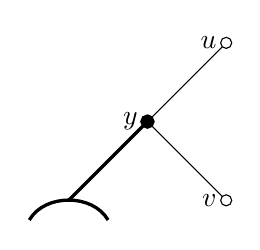
\begin{tikzpicture}[scale=1]
\draw (0,1)--(-1,-0)--(0,-1);
\draw[fill=white] (0,1) circle [radius=2pt]
(0,-1) circle [radius=2pt];
\draw[very thick,fill=black] (-1,0) circle [radius=2pt] (-1,0)--(-2,-1);
\draw[very thick] (-2.5,-1.25) to[out=60,in=120] (-1.5,-1.25);
\node[left] at (0,1) {$u$};
\node[left] at (-1,0) {$y$};
\node[left] at (0,-1) {$v$};
\end{tikzpicture}
\subcaption{$(Y,left)$~left.}
\end{minipage}
\begin{minipage}{0.2\textwidth}
\centering
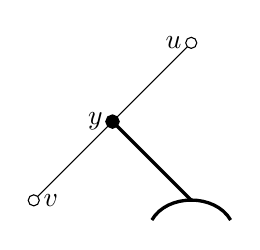
\begin{tikzpicture}[scale=1]
\draw (0,1)--(-2,-1);
\draw[fill=white] (0,1) circle [radius=2pt]
(-2,-1) circle [radius=2pt];
\draw[very thick,fill=black] (-1,0) circle [radius=2pt] (-1,0)--(0,-1);
\draw[very thick] (-0.5,-1.25) to[out=60,in=120] (0.5,-1.25);
\node[left] at (0,1) {$u$};
\node[left] at (-1,0) {$y$};
\node[right] at (-2,-1) {$v$};
\end{tikzpicture}
\subcaption{$(Y,right)$~left.}
\end{minipage}
\begin{minipage}{0.25\textwidth}
\centering
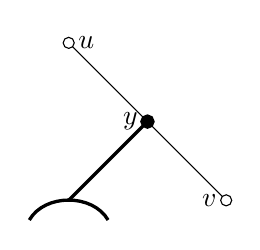
\begin{tikzpicture}[scale=1]
\draw (-2,1)--(0,-1);
\draw[fill=white] (-2,1) circle [radius=2pt]
(0,-1) circle [radius=2pt];
\draw[very thick,fill=black] (-1,0) circle [radius=2pt] (-1,0)--(-2,-1);
\draw[very thick] (-2.5,-1.25) to[out=60,in=120] (-1.5,-1.25);
\node[right] at (-2,1) {$u$};
\node[left] at (-1,0) {$y$};
\node[left] at (0,-1) {$v$};
\end{tikzpicture}
\subcaption{$(Y,left)$~right.}
\end{minipage}
\begin{minipage}{0.2\textwidth}
\centering
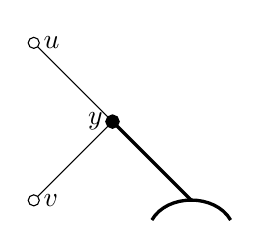
\begin{tikzpicture}[scale=1]
\draw (-2,1)--(-1,0)--(-2,-1);
\draw[fill=white] (-2,1) circle [radius=2pt]
(-2,-1) circle [radius=2pt];
\draw[very thick,fill=black] (-1,0) circle [radius=2pt] (-1,0)--(0,-1);
\draw[very thick] (-0.5,-1.25) to[out=60,in=120] (0.5,-1.25);
\node[right] at (-2,1) {$u$};
\node[left] at (-1,0) {$y$};
\node[right] at (-2,-1) {$v$};
\end{tikzpicture}
\subcaption{$(Y,right)$~right.}
\end{minipage}
\caption{The drawings describe the plug in operation in the different four cases. The bold part highlight the single pair $(Y,S)$.}
\label{fig:plugin}
\end{figure}

Let $(Y,S)$ be a single pair in a rooted subcubic tree $T$, then we {\it remove} $(Y,S)$ from $T$ as follows. Let $y$ be the root of $Y$. If $y$ is the root of $T$, then we obtain an empty tree. If $y$ is a leaf node of $T$, then we obtain $T-y$. Otherwise let $y$ be a non-root and non-leaf node, let $u$ be the parent of $y$ and $v$ be the child of $y$ that is not in $V(Y)$, then we consider the tree obtained from $T$ after replacing $y$ with $v$ as the child of $u$ and deleting $Y$. See Figure~\ref{fig:reduction} for an example.

\begin{figure}[h]
\begin{minipage}{0.5\textwidth}
\centering
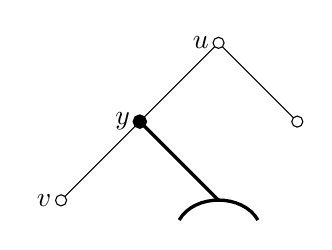
\begin{tikzpicture}[scale=1]
\draw (0,1)--(-2,-1) (0,1)--(1,0);
\draw[fill=white] (0,1) circle [radius=2pt]
(1,0) circle [radius=2pt]
(-2,-1) circle [radius=2pt];
\draw[very thick,fill=black] (-1,0) circle [radius=2pt] (-1,0)--(0,-1);
\draw[very thick] (-0.5,-1.25) to[out=60,in=120] (0.5,-1.25);
\node[left] at (0,1) {$u$};
\node[left] at (-1,0) {$y$};
\node[left] at (-2,-1) {$v$};
\end{tikzpicture}
\end{minipage}
\begin{minipage}{0.1\textwidth}
\centering
\begin{tikzpicture}[scale=1]
\draw (0,1)--(-2,-1) (0,1)--(1,0);
\draw[fill=white] (0,1) circle [radius=2pt]
(1,0) circle [radius=2pt]
(-2,-1) circle [radius=2pt];
\node[left] at (0,1) {$u$};
\node[left] at (-2,-1) {$v$};;
\end{tikzpicture}
\end{minipage}
\caption{The drawing describe an example of the remove operation: a single pair $(Y,right)$ is removed from a subcubic rooted tree. The bold part highlight the single pair $(Y,S)$.}\label{fig:reduction}
\end{figure}

It is clear from the four different plug in cases that if we want to plug in two pairs $(Y,S)$ and $(Y',S')$ on an edge $uv$ such that the ancestor-descendant relationship is given, say $y$ of $Y$ has to be in the path from the root to $y'$ of $Y'$, then we can do these plug ins in any order but with some care. It is the same if we first plug in $(Y,S)$ in the edge $uv$ and then plug in $(Y',S')$ in the edge $yv$ or if we first plug in $(Y',S')$ in the edge $uv$ and then plug in $(Y,S)$ in the edge $uy'$. See Figure~\ref{fig:multiplugin} for the an example.

\begin{figure}[h]
\centering
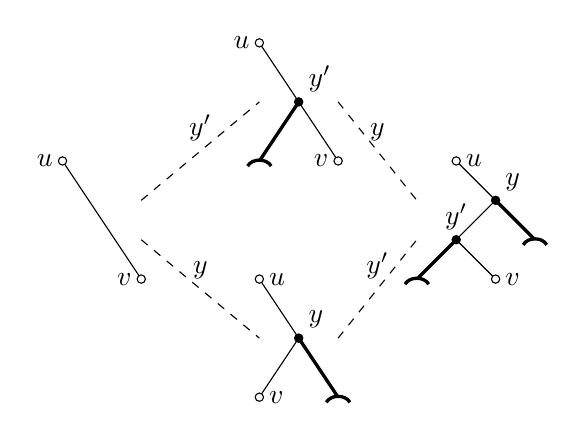
\begin{tikzpicture}[scale=0.5]
\draw[dashed] (-5,0)--(-2,2.5) node[midway,above] {$y'$}
(-5,-1)--(-2,-3.5) node[midway,above] {$y$}
(0,2.5)--(2,0) node[midway,above] {$y$}
(0,-3.5)--(2,-1) node[midway,above] {$y'$};
\draw (-7,1)--(-5,-2) (-2,4)--(0,1) (-2,-2)--(-1,-3.5)--(-2,-5) (3,1)--(4,0)--(3,-1)--(4,-2);
\draw[very thick] (-1,-3.5)--(0,-5) (-1,2.5)--(-2,1) (4,0)--(5,-1) (3,-1)--(2,-2) (-2.3,0.87) to[out=60,in=120] (-1.7,0.87)
(-0.3,-5.13) to[out=60,in=120] (0.3,-5.13) (4.7,-1.13) to[out=60,in=120] (5.3,-1.13) (1.7,-2.13) to[out=60,in=120] (2.3,-2.13);
\draw[fill=white] (-7,1) circle [radius=3pt] (-5,-2) circle [radius=3pt] (-2,4) circle [radius=3pt] (0,1) circle [radius=3pt] (-2,-2) circle [radius=3pt] (-2,-5) circle [radius=3pt] (3,1) circle [radius=3pt] (4,-2) circle [radius=3pt];
\draw[fill=black] (-1,-3.5) circle [radius=3pt] (-1,2.5) circle [radius=3pt] (4,0) circle [radius=3pt] (3,-1) circle [radius=3pt];
\node[left] at (-7,1) {$u$};
\node[left] at (-2,4) {$u$};
\node[right] at (-2,-2) {$u$};
\node[right] at (3,1) {$u$};
\node[left] at (-5,-2) {$v$};
\node[left] at (0,1) {$v$};
\node[right] at (-2,-5) {$v$};
\node[right] at (4,-2) {$v$};
\node[above right] at (4,0) {$y$};
\node[above right] at (-1,-3.5) {$y$};
\node[above right] at (-1,2.5) {$y'$};
\node[above] at (3,-1) {$y'$};
\end{tikzpicture}
\caption{An example of plugging in two pairs $(Y,left)$ and $(Y',right)$ in a left edge $uv$.}
\label{fig:multiplugin}
\end{figure}

For a subset of labels $A\subseteq [k]$, we define the feature template $f_A$ by setting $e(f_A)=1$ if and only if $lab(e)\in A$ and $e(f_A)=0$ otherwise. With a small abuse of notation, we often identify the feature template $f_A$ with the corresponding subset of labels $A$.

\smallskip
Suppose we have a DT such that some feature label~$i$ occurs twice on a path from the root to the leaves, say~$f_1$ is the instance closer to the root and~$f_2$ is the other instance. If~$f_2$ is in the left (resp. right) subtree of~$f_1$, we remove $f_2$'s right (resp. left) subtree. In this case we say we have done an {\it actual removal}.

Suppose we have a feature template labelled~$A$ in our decision tree. Let $A_1,\ldots,A_\ell$ be the sequence of feature templates on the path from the root to~$A$ in order (not including~$A$). Let $A_i'=A_i$ if~$A$ is in the right sub-tree of~$A_i$ and let $A_i'=\overline{A_i}$ otherwise. If $\overline{A} \subseteq A_1' \cup \ldots \cup A_\ell'$, then we remove the subtree rooted at the left child of~$A$. If $A\subseteq \overline{A_1'} \cup \ldots \cup \overline{A_\ell'}$, then we remove the subtree rooted at the right child of~$A$. In this case we say we have done a {\it template removal}. If this procedure has been applied to a record exhaustively, we say that the DT is {\it reduced}.

To be short, for a DT $T$ and a node $v$, we write $v\in T$ instead of $v\in V(T)$ and $v\not\in T$ otherwise.

We now formally define two important operations. Given a DT $T$, we say that we {\it reduce} $T$ if we exhaustively do actual removals and template removals. Call $r(T)$ the resulting DT.

Recall that in any DT $T$, every non-leaf node $v$ has one of the following three contents: $v$ is a real feature (without label), or $v$ is a feature with a label, or $v$ is a future feature with the corresponding subset of labels.
A {\it relabelling} $p$ for $T$ is an assignment of contents of $T$ as follows. Every feature is assigned to a feature with is either future, real or with a label. We say that we {\it relabel} the DT $T$ via the relabelling $p$ if for every node of $T$ we apply the corresponding assignment and call $p(T)$ the resulting DT.

The following lemma shows that, after repeatedly applying it the necessary amount of times, to obtain a reduced DT after a sequence of relabels, it is safe to reduce at the end.

\begin{lemma}[Relabelling Lemma]\label{red-last}
Let $T$ be a DT and $p$ be relabelling of $T$. Then $(r \circ p \circ r) (T)=(r \circ p) (T)$.
\end{lemma}

\begin{proof}
For every $v\in T$, we want to prove $v\in (r\circ p\circ r)(T) \Leftrightarrow v\in (r \circ p)(T)$.

$\Rightarrow$ Suppose there is a node $v\not\in (r \circ p)(T)$. Since $v\in p(T)$, there is a set of ancestors of $v$ in $p(T)$ that allows to remove $v$. Let $A_v$ be the union of all the minimal set of ancestors of $v$ in $p(T)$ that allows to remove $v$. If $A_v$ is a set of ancestors of $v$ in $T$ that allows to reduce $v$ then $v\not\in r(T)$ and so $v\not \in (r\circ p\circ r)(T)$. Otherwise let $A'_v$ be the subset of $A_v$ in $(p \circ r)(T)$. We conclude by noting that $A'_v$ contains one of the minimal sets $A_v$ is composed of and so $v\not \in (r\circ p\circ r)(T)$.

$\Leftarrow$ Suppose there is a node $v\not\in (r \circ p \circ r)(T)$. If $v\in (p \circ r)(T)$, there exists a set $A_v$ of ancestors of $v$ in $(p \circ r)(T)$ that allows to reduce $v$. Then $A_v$ is a set of ancestors of $v$ in $p(T)$ that allows to reduce $v$ and so $v\not\in (r \circ p)(T)$. If $v\not\in (p \circ r)(T)$ then $v\not\in r(T)$: there exists a set $A_v$ of ancestors of $v$ in $T$ that allows to remove $v$. This means $A_v$ is a set of ancestors of $v$ in $p(T)$ that allows to remove $v$ and so $v\not\in (r \circ p)(T)$.
\end{proof}

We say that a DT $T$ is a {\it real DT} if every non-leaf node is either a real feature or a future feature, whereas it is a {\it DT template} if it contains no real feature.

Let $B$ be a rooted subcubic tree that corresponds to a $k$-NLC expression of the graph $G_I(E)$.
For $b\in V(B)$, we write $feat(b)$ and $exam(b)$ for the sets of features and examples introduced at nobe $b$.
We say that a real DT $T$ is a DT for the node $b$ if every real feature of $T$ is an element of $feat(b)$ and every example in $exam(b)$ is correctly classified by $T$, i.e. if $e\in exam(b)\cap E^+$ then $e$ ends in a leaf with a $+$ label and if $e\in exam(b)\cap E^-$ then $e$ ends in a leaf with a $-$ label.

Given a real DT $T$ and a node $b\in B$, often we want to perform a very specific composition of operations. Let $p_b$ be the following relabelling of $T$: every real feature of $T$ is assigned to a feature with the label given by the $k$-NLC expression at node $b$ and every other feature is assigned to itself. Then the composition $r \circ p_b$ is called the {\it standard reduction} of $T$ at node $b$.
Given a DT $T$ and a node $b\in B$, it is useful to give the following relabelling $p'_b$: every feature with a label is assigned to the real feature of that node. The relabelling $p'_b$ is called the {\it real relabelling} of $T$ at node $b$.

We say that a DT template $T$ is a DT for the node $b$ if there exits a real DT $T'$ for $b$ such that $T$ is the standard reduction of $T'$. In this case we say that $T'$ is the witness of $T$ for $b$.

\begin{comment}
\smallskip
A {\it record} for a node $b\in V(B)$ is a pair $(T,s)$, where:

\begin{itemize}
\item $T$ is a {\it reduced} DT consisting of
\begin{itemize}
\item actual feature nodes with labels in $[k]$;
\item future feature nodes with labels in $\mathcal{P}[k]$;
\item leaf nodes with labels in $\{+,-\}$.
\end{itemize}
\item $s\in \mathbb{N}$ is the number of all the elements that have been deleted as the result of a series of remove operations from a DT $T'$ for $b$ to obtain $T$. 
\end{itemize}
\end{comment}

\begin{comment}
\begin{lemma}\label{lem:reduced-tree-height}
If there are $\ell$ actual feature labels and $2^k$ future template labels, then every reduced DT has height at most~$\ell+k$. Furthermore, every path from the root to the leaves contains at most~$\ell$ actual feature labels and at most $k-1$ future feature templates.
\end{lemma}

\begin{proof}
Consider a path~$P$ of maximum length from the root to the leaves in a reduced DT $T$. No actual feature label appears more than once on this path, so the number of actual feature nodes on this path is at most~$\ell$. Consider two future features $f_{A}$ and $f_{A'}$ that appear in $P$, say $f_{A}$ is the instance closer to the root. Since $T$ is reduced, we must have that $\emptyset\subset A'\subset A$. Since the label of any future feature has at most $k$ elements, there can be at most $k-1$ feature template nodes on this path. The path ends with a leaf node, so this gives a total of $\ell+k-1+1=\ell+k$ nodes, as required.
\end{proof}

\begin{lemma}\label{lem:reduced-tree-number}
If there are $\ell$ actual feature labels and $2^k$ future template labels, then there are at most $(\ell+2^k+2)2^{\ell+k+1}$ reduced DTs. Furthermore, these can be enumerated in $\mathcal{O}((\ell+2^k+2)2^{\ell+k+1})$-time.
\end{lemma}

\begin{proof}
There are~$\ell$ actual feature labels and $2^k$ possible future template labels and leaves can be either positive or negative.
By Lemma~\ref{lem:reduced-tree-height}, the tree has height at most $\ell+k$.
Each node of the decision tree could be a feature label, a future feature template, or a leaf (in which case it has no children), there are at m t $\ell+k$, there are at most $2^{\ell+k+1}$ nodes in the tree, so there are at most $(\ell+2^k+2) 2^{\ell+k+1}$ possible decision trees.
\end{proof}
\end{comment}

\smallskip
The {\it semantics} for a record are defined as follows. We say that a pair $(T,s)$ is a {\it record} for the node $b\in B$ and we write $(T,s)\in \mathcal{R}(b)$, if $T$ is a DT template for $b$ and $s$ is the minimum number of elements that have been deleted from a witness $T'$ of $T$ for $b$.

Now, it suffices to compute $\mathcal{R}(b)$ via leaf-to-root dynamic programming. The following four lemmas show how this can be achieved for all of the four types of nodes in a $k$-NLC expression tree $B$.

\begin{lemma}\label{lem:leaf}
Let $b\in V(B)$ be a leaf node. Then $\mathcal{R}(b)$ can be computed in time $\mathcal{O}()$.
\end{lemma}

\begin{proof}
Let $v$ be the vertex of $G_I(E)$ that corresponds to the leaf node $b$. This means either $v\in E$ or $v\in feat(E)$.

We have to enumerate all possible reduced DT templates $T$ for $b$. It is enough to consider all reduced DT templates $T$ of height at most $k+1$ and discard those that are not DT templates for $b$; these are at most $()$ by Lemma~\ref{lem:reduced-tree-number}. We add the pair $(T,0)$ to the set of records $\mathcal{R}(b)$. 

Now we have to show the correctness of the construction for $\mathcal{R}(b)$, i.e. $(T,s)\in \mathcal{R}(b)$ if and only if $s$ is the minimum number of elements that have been deleted from a witness $T'$ of $T$ for $b$.

We start with the forward direction. Let $(T,s)\in \mathcal{R}(b)$. By construction, we have that $s=0$ and $T$ is a DT template for $b$ which is already reduced. Then $T$ is trivially a witness of $T$ for $b$.

Now we prove the backward direction. Let $T$ be a reduced DT template such that $0$ is the minimum number of elements that have been deleted from a witness $T'$ of $T$ for $b$. This means $T'$ is obtained from $T$ after the real relabelling at node $b$ is applied: $T$ is a DT template among the considered DTs above which leads to the fact that $(T,0)\in \mathcal{R}(b)$.
\end{proof}

\begin{lemma}\label{lem:join}
Let $b\in V(B)$ be a join node. Then $\mathcal{R}(b)$ can be computed in time $\mathcal{O}()$.
\end{lemma}

\begin{proof}
Let $b_L$ and $b_R$ be the left, resp. right, child of $b$ in $B$: we may assume the labels for $feat(b_L)$ are in $[k]$ and the labels for $feat(b_R)$ are in $[k']$. Moreover, let $M$ be the $k\times k$ $\{0,1\}$ matrix that represent the node $b$. Finally, for every label $i\in [k]$, let $A_i=\{j\in [k]~|~M_{i,j}=1\}$.

We consider every reduced DT $T$ for $b$ with feature labels in $[k]\cup [k']$ and future feature labels in $\mathcal{P}([k])$; these are at most $()$ by Lemma~\ref{lem:reduced-tree-number}.

For every such DT $T$, we create a DT $T_L$ as follows. Let $p_*$ be the following relabelling: for every $i'\in [k']$, every feature with label $i'$ is assigned to the future feature $A_i$. Then we apply the composition $r \circ p_*$ to $T$. In a symmetrical way we create a DT $T_R$. Let $p'_*$ be the following relabelling: for every $i\in [k]$, every feature with label $i$ is assigned to the future feature $A_i$. Then we apply the composition $r \circ p'_*$ to $T$.

Now we want to understand if there is a record in $\mathcal{R}(b_L)$ of the form $(T_L,s_L)$ for some positive integer $s_L$ and if there is a record in $\mathcal{R}(b_R)$ of the form $(T_R,s_R)$ for some positive integer $s_R$: if the answer is yes in both cases, we add a record $(T,s_L+s_R)$ to $\mathcal{R}(b)$; otherwise we discard this option.

\medskip
Now we have to show the correctness of the construction for $\mathcal{R}(b)$. We start with the forward direction. Let $(T,s)\in \mathcal{R}(b)$. By construction there exist records $(T_L,s_L)\in \mathcal{R}(b_L)$ and $(T_R,s_R)\in \mathcal{R}(b_R)$ such that $T_L$ and $T_R$ are obtained by the application of $r \circ p_*$ and $r \circ p'_*$ respectively to $T$ and $s_L+s_R=s$.

By induction, for $H\in \{L,R\}$, we know that $s_H$ is the minimum number of elements that have been deleted from a witness $T'_H$ of $T_H$ for $b_H$.

For $H\in \{L,R\}$, we define maps $x_H$ and $y_H$ as follows. Let $x_H~:~V(T_H)\to V(T)$ and $y_H~:~V(T_H)\to V(T'_L)$ be the functions that maps every node of $T_H$ to the corresponding node in $T$ and in $T'_L$ and note that by constructions both these maps are injective. 

\begin{figure}[h]
\centering
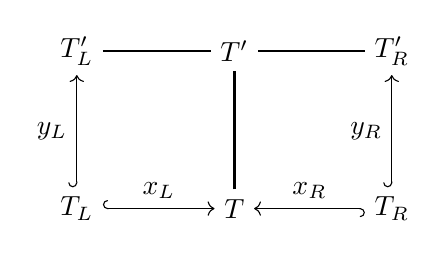
\begin{tikzpicture}
\node (1) at (-2,1) {$T'_L$};
\node (2) at (0,1) {$T'$};
\node (3) at (2,1) {$T'_R$};
\node (4) at (-2,-1) {$T_L$};
\node (5) at (0,-1) {$T$};
\node (6) at (2,-1) {$T_R$};
\draw[right hook->] (4)--(5) node[midway,above] {$x_L$};
\draw[right hook->] (6)--(5) node[midway,above] {$x_R$};
\draw[right hook->] (4)--(1) node[midway,left] {$y_L$};
\draw[right hook->] (6)--(3) node[midway,left] {$y_R$};
\draw[thick] (1)--(2);
\draw[thick] (3)--(2);
\draw[very thick] (5)--(2);
\end{tikzpicture}
\end{figure}

Moreover, $V(T)\setminus Im(x_H)$ and $V(T'_H)\setminus Im(y_H)$ can be partitioned into subtrees that have been deleted after the application of $r\circ p_*$, $r\circ p'_*$ on $T$ or of the standard reduction on $T'_H$: let $X^*_H=\{x^H_1,\ldots,x^H_\ell\}$ and $Y^*_H=\{y^H_1,\ldots,y^H_r\}$ be the set of roots of the above subtrees in $V(T)\setminus Im(x_H)$ and $V(T'_H)\setminus Im(y_H)$ respectively.  In addition, for every $i$, let $Y^H_i$ be the maximal subtree of $T'_H$ rooted at $y^H_i$ with no elements from $Im(y_H)$ and that does not contain any vertex from $Y^*_H\setminus \{y^H_i\}$; let $(Y^H_i,S^H_i)$ the corresponding single pair. In a similar way, for every $i$, let $X^H_i$ be the maximal subtree of $T$ rooted at $x^H_i$ with no elements from $Im(x_H)$ and that does not contain any vertex from $X^*_H\setminus \{x^H_i\}$; let $(X^H_i,S^H_i)$ the corresponding single pair. Finally, for any $i$, let $p^H_i$ be the shortest downwards path in $T'_H$ that contains $y^H_i$ and with both endpoints in $Im(y_H)$, say $y_H(v_1)$ and $y_H(v_2)$. 

\smallskip
\noindent
{\it Claim 1: For every $H\in \{L,R\}$ and for every $i,j\in [r]$, the paths $p^H_i$ and $p^H_j$ are either edge disjoint or $p^H_i=p^H_j$.}

\noindent
{\it Proof.} If $p^H_i$ and $p^H_j$ are edge disjoint, then the statement is proven immediately. Suppose $p^H_i$ and $p^H_j$ share an edge. By minimality and the fact they are downwards paths, $p^H_i$ and $p^H_j$ share the endpoint towards the root. If they also share the other endpoint, then the statement is proven immediately. Suppose now their endpoints towards the leaves is different, say $v_i$ and $v_j$, and consider the last edge those paths have in common in a descending order, say $uv$. 

Without loss of generality, we can assume $v_i$ belongs to the left branch of $v$ and $v_j$ belongs to the right branch of $v$. Note that $v\in V(T'_H)\setminus Im(y_H)$, or we get a contradiction due the minimality of $p^H_i$.
Now we get the following contradiction: by construction, $v_i$ and $v_j$ are both elements of $Im(y_H)$ but at least one of them must be in $V(T'_H)\setminus Im(y_H)$ since it is an element of either $Y^H_i$ or of $Y^H_j$. This proves Claim 1.

\smallskip
Now we consider the path $q^H_i$ in $T$ having endpoints $x_H(v_1)$ and $x_H(v_2)$.

\smallskip
\noindent
{\it Claim 2: For every $H\in \{L,R\}$ and for every $i\in [r]$, every internal vertex of $q^H_i$ is an element of $X^*_H$.}

\noindent
{\it Proof.} Suppose that $q^H_i$ has an internal vertex $t\not\in X^*_H$. By definition, there exists a vertex $v\in V(T_H)$ such that $x_H(v)=t$. Since $x_H$ is injective then $v\not\in \{v_1,v_2\}$. Since $y_H$ is injective $y_H(v)\not\in \{y_H(v_1),y_H(v_2)\}$ and belongs to $p_i$, which contradicts the minimality of $p_i$. This proves Claim 2.

\smallskip
Before we describe how to obtain a witness $T'$ of $T$ for $b$, we must make an observation. We note that $Im(x_L)\cup Im(x_R)=V(T)$: the idea is that every node of $T$ must originate from either $T_L$ or $T_R$.

%We, now, show that when there is a sequence of relabelling and consequent reductions, these can be done in any order without affecting the resulting DT and total score of the reductions. To do so, we consider the operation of relabelling two nodes and applying the reduction algorithm in a DT: by repeating this operation the proper amount of times, this gives proof for the general case. Suppose $T$ is a reduced DT and let $u$ and $v$ be two of his nodes. Recall that a relabel and reduce operation at a node $w$, in short call it  $r(w)$, influences only the nodes in $T_w$, that is the subtree of $T$ rooted at $w$. To be short, we write that $v'\in r(v)$ if a node $v'$ is present after $r(v)$ and write $v'\notin r(v)$ otherwise.
%If $u$ is neither a descendant or an ancestor of $v$ then $T_u$ and $T_v$ are disjoint an so $r(u)$ and $r(v)$ commutes. Without loss of generality we can suppose $v$ is a node of $T_u$, that is $u$ is an ancestor of $v$. 
%$Suppose there is a node $v^*\in r(v) \circ r(u)$ but $v^*\not\in r(u) \circ r(v)$. If $v^*\not\in r(v)$ then, since $v^*\in r(v) \circ r(u)$, $r(u)$ has removed some nodes that allowed to remove $v^*$ and so $v^*$ could be removed as well, that is $v^*\not\in r(u)$ which is a contraddiction. If $v^*\in r(v)$ then $v^*\not\in r(u)$ which is again a contraddiction. By symmetry we have that, for any $u,v,v^*\in T$, $v^*\in r(v) \circ r(u)$ if and only if $v^*\in r(u) \circ r(v)$ and so $r(u)$ and $r(v)$ commute.

\smallskip
Now we are able to describe how to obtain a witness $T'$ of $T$ for $b$. For every $i\in [r]$, we consider the internal vertices $\{y_{i_1},\ldots,y_{i_t}\}$ of $p^L_i$, that we recall belong to $Y^*_L$, in a descending order. In the path $q^L_i$, we plug in, in sequence, every single pair $(Y^L_{i_j},S^L_{i_j})$ rooted at $y_{i_j}$ with $j\in [t]$ in the last edge of the path $q^L_i$. Note that, in the case an element of $Y^*_L$ is present in more than one $p^L_i$, we plug in the corresponding single pair only once. Note also that whenever we plug in some single pair $(Y^L_{i_j},S^L_{i_j})$ in a DT, the tree $Y^L_{i_j}$ has real features and future features as nodes. Call this graph $T^*$. Now we do the same sequence of plug ins of the single pairs corresponding to the internal vertices of $p^R_i$ in the last edge of the path $q^R_i$. Again, in the case an element of $Y^*_R$ is present in more than one $p^R_i$, we plug in the corresponding single pair only once. Call the tree obtained in this way $T'$. Node that $T'$ contains real features from $feat(b_L)$ and from $feat(b_R)$ and future features with labels in $\mathcal{P}([k])$.

\smallskip
To conclude this part of the proof we have to show two things: $(i)$ $T$ is obtained from $T'$ after removing $s$ vertices; $(ii)$ $T'$ is a real DT for $b$. We start proving $(i)$: by construction $T'$ is obtained from $T$ after adding $s_L$ elements from $T'_L$ and $s_R$ elements from $T'_R$, and so with $s_L+s_R=s$ more elements. 

Before considering statement $(ii)$, we consider the following relabelling $p_+$ of $T'$: every real feature in $feat(b_R)$ is a assigned to a feature with its label at node $b_R$ and every other feature is assigned to itself. The real DT $T'_L$ can be obtained from $T'$ by the application of the composition $r \circ p_* \circ p_+$.

Now we consider statement $(ii)$. We show that given an example $e\in exam(b_L)$, $e$ is correctly classified by $T'$ and to do so we show that $e$ ends in a leaf of $T'$ that corresponds to the leaf where $e$ ends in $T'_L$. 
Say that $e$ goes along a path $P$ of $T'_L$ from the root to a leaf $\ell$ and let $Q$ be the corresponding path $T'$, i.e. the from the root $r$ to $\ell$ (note that by construction $\ell$ is present in $T'$ and is still a leaf). 
Let $v$ be a node of $Q$, we can have the following different cases.

\begin{itemize}
\item $v$ is a real feature from $feat(b_L)$: $v$ is also present in $T'_L$ as real feature; 
\item $v$ is a real feature from $feat(b_R)$: $v$ might not be present in $T'_L$ due reductions but if it is present it is a future feature $A_i$ for some $i\in [k]$;
\item $v$ is a future feature $f_A$: $v$ might not be present in $T'_L$ due reductions but if it is present it is still the same future feature $A_i$.
\end{itemize}

If $v$ is present in $T'_L$ then the behaviour of $v$ on $e$ in $T'_L$ and in $T'$ is the same. Suppose now $v$ is a node of $Q$ that is being reduced due his label and so it is not present in $T'_L$. This means there is a set of ancestors of $v$ such that their labels allows to remove $v$ and by construction $v$ behaves on $e$ like those ancestors. This proves $e$ goes along $Q$ and in particular it ends at leaf $\ell$ and so $T'$ is a real DT for $b_L$. With symmetric construction, we show that $T'$ is also a real DT for $b_R$.

\medskip
Now we prove the backward direction. Let $T$ be a reduced DT such that $s$ is the minimum number of elements that have been deleted from a witness $T'$ of $T$ for $b$. In particular, we recall that $T'$ is a real DT for $b$ with actual feature labels in $[k]\cup [k']$ and future feature labels in $\mathcal{P}([k])$. 

We create at real DT $T'_L$ by the application of the composition $r \circ p_* \circ p_+$ to $T'$. By assumption $T'$ is a real DT for $b_L$ and by construction $T'_L$ is a real DT for $b_L$. 
Denote with $T_L$ the DT template obtained from $T'_L$ by standard reduction and denote with $s_L$ the number of nodes that have been deleted from $T'_L$ to obtain $T$. By induction we have $(T_L,s_L)\in \mathcal{R}(b_L)$.
Now we note that $T_L$ is obtained from $T$ after the application of the composition $r \circ p_*$. In a symmetric way, we construct $T'_R$, $T_R$ and the record $(T_R,s_R)\in \mathcal{R}(b_R)$. Then $(T,s_L+s_R)\in \mathcal{R}(b)$.
\end{proof}

\begin{lemma}\label{lem:relabel}
Let $b\in V(B)$ be relabelling node. Then $\mathcal{R}(b)$ can be computed in time $\mathcal{O}()$.
\end{lemma}

\begin{proof}
Let $b_C$ be the unique child of $b$ in $B$. Let $R$ be the mapping of $[k]$ to itself that represent the node $b$. Moreover, since we are considering a {\it nice} NLC-expression we can assume $R$ is the identity mapping, i.e. $R(\ell)=\ell$, for all values except for a unique element $i$ of its domain, i.e. $R(i)=j$ for some $j\in [k]\setminus \{i\}$.

We say that a future feature $A$ is {\it good} if it does not distinguish between $i$ and $j$, that is $i\in A$ if and only if $j\in A$, and {\it bad} otherwise. Let $(T_C,s_C)$ be an element of $\mathcal{R}(b_C)$. Let $p''$ the following relabelling of the DT template $T_C$: every feature with label $i$ is assigned to label $j$ and every future feature with label $A$ is assigned to the future feature with label $A\setminus \{i\}$. 

If $T_C$ has a bad future feature then we do not take any other action. Suppose now $T_C$ has only good future features; now let $T$ be the DT template obtained from $T_C$ after the application of the composition $r \circ p''$ and let $s^*$ be the number of nodes that have been deleted from $T_C$ to $T$.

If there is a record in $\mathcal{R}(b)$ of the form $(T,s')$ for some integer $s'\leq s_C+s^*$ then we do not take any other action.
If there is a record in $\mathcal{R}(b)$ of the form $(T,s')$ for some integer $s'>s_C+s^*$ then we replace it with $(T,s_C+s^*)$.
If there is no record in $\mathcal{R}(b)$ of the form $(T,s')$ for some integer $s'$ then we add $(T,s_C+s^*)$ to $\mathcal{R}(b)$.

\medskip
Now we have to show the correctness of the construction for $\mathcal{R}(b)$, i.e. $(T,s)\in \mathcal{R}(b)$ if and only if $s$ is the minimum number of elements that have been deleted from a witness $T'$ of $T$ for $b$.

\smallskip
We start with the forward direction. Let $(T,s)\in \mathcal{R}(b)$. By construction there exists a record $(T_C,s_C)\in \mathcal{R}(b_C)$ such that $T$ is obtained from $T_C$ after the application of $r \circ p''$ and let $s^*=s-s_C$. By induction $s_C$ is the minimum amount of nodes that have been deleted from a witness $T'_C$ of $T_C$ for $b_C$. By construction we also know that every future feature of both $T'_C$ and $T_C$ is good.

Denote with $T'$ the real DT obtained $T'_C$ after the application of $r \circ p''$: note that this last reduction does not any node since every future feature of $T'_C$ is good and there is no feature with label $i$. To conclude this part of the proof we have to show two things: $(i)$ $T$ is obtained from $T'$ after removing $s$ vertices; $(ii)$ $T'$ is a witness of $T$ for $b$. 

Before proving $(i)$, we describe how $T$ can be obtained from $T'$. Let $p'''$ be the following relabelling of $T'$: every real feature that contains $j$ is assigned to the real feature $A\cup \{i\}$ and every other feature is assigned to itself. Then the application of the composition $p'''$, the standard reduction and $r \circ p''$ to $T'$ is exactly the standard reduction for $T'$ which then result to the DT template $T$.
By Lemma~\ref{red-last} the score of the standard reduction from $T'$ to $T$ is exactly $s_C+s^*=s$. 

Now we consider statement $(ii)$. First note that $exam(b)=exam(b_C)$.
We show that a given example $e\in exam(b)$ is correctly classified by $T'$. Say that $e$ goes along a path $P$ of $T'_C$ from the root to a leaf $\ell$. We show $e$ goes along the path $P$ in $T'$ as well: every real feature has not changed and so $e$ behaves the same. Since every future feature of $T'_C$ is good, then $e$ behave the same on the corresponding future feature of $T'$.

\smallskip
Now we prove the backward direction. Let $T$ be a reduced DT such that $s$ is the minimum number of elements that have been deleted from a witness $T'$ of $B$ for $b$. In particular, we recall that real $T'$ is a DT for $b$ with real features and future feature labels in $\mathcal{P}([k]\setminus \{i\})$.

We create the real DT $T'_C$ as the application of $r \circ p'''$ to $T'$, the DT template $T_C$ as the application of the standard reduction to $T'_C$. By construction we have $(T_C,s_C)\in \mathcal{R}(b_C)$, where $s_C$ is the number of nodes that have been removed from $T'_C$ to $T_C$. Note that $T_C$ has only good future features.
Finally we note that $T$ is obtained from $T_C$ by the application of $r \circ p''$.
\end{proof}

\begin{comment}
\begin{lemma}
Let $b\in V(B)$ be the root node. Then $\mathcal{R}(b)$ can be computed in time $\mathcal{O}()$.
\end{lemma}

\begin{proof}
By the nature of NLC decomposition, $b$ is either a leaf or a join or a relabelling node, so the running time to compute $\mathcal{R}(b)$ is the obtained from Lemmas~\ref{lem:leaf}, \ref{lem:join} and \ref{lem:relabel}. To conclude, we want to select a record $(T,s)\in \mathcal{R}(b)$ such that $s$ is minimum over all DTs with no future features.
\end{proof}
\end{comment}



\end{document}



%
%\subsection{Story Line}
%\begin{enumerate}
%\item DT important for ML
%\item Small trees (low depth!) good for XAI
%\item Contribution: new method for learning significantly smaller DTs
%  with almost same accuracy based on
%  \begin{enumerate}
%  \item \emph{new partition-based SAT-encoding for optimizing depth }
%    Fundamentally different and better for our purpose than existing
%    encodings (Avellaneda, Janota) because:
%    \begin{itemize}
%    \item Encoding size depends on number of experiments
%    \item Robust wrt \#features, depth (asymptotical argument)
%    \item Easy to extend to nonbinary decisions and feature values
%    \item Use Avellaneda for smaller instances
%    \end{itemize}
%  \item \emph{new incremental learning procedure/scheme}
%    Compare 3 strategies
%  \end{enumerate}
%
%\item Experimental results
%\end{enumerate}



%%% Local Variables:
%%% mode: latex
%%% TeX-master: t
%%% End:

%\begin{table}
%\begin{tabular}{l l l |rrr|rrr|rr|rr|r} 
%\toprule
%& &   & \multicolumn{6}{c|}{Incremental} & \multicolumn{4}{c|}{Extending} &  \\
%& & & \multicolumn{3}{c|}{\stratrand} & \multicolumn{3}{c|}{\stratinc} & 
%\multicolumn{2}{c|}{\stratrand} & \multicolumn{2}{c|}{\stratleaf} &
%\multicolumn{1}{c}{ITI}\\ 
%Instance & IR & CR
%&$a$	&$a_u$	&$d$
%&$a$	&$a_u$	&$d$
%&$d_h$	&$d_c$
%&$d_h$	&$d_c$
%&$d$\\
%
%\midrule
%appendicitis		&F&F&0.86	&0.86	&3	&0.81	&0.81	&2	&33&15	&25&15	&12\\
%			&F&T&0.93	&0.93	&12	&0.85	&0.85	&3	&27&13	&15&12	&\\
%			&T&F&1.00	&1.00	&15	&1.00	&1.00	&15	&15&15	&-&15	&16\\
%			&T&T&1.00	&1.00	&15	&1.00	&1.00	&15	&15&15	&-&15	&\\
%\midrule
%australian		&F&F&0.86	&0.86	&2	&0.80	&0.80	&3	&13&-	&14&-	&16\\
%			&F&T&0.86	&0.86	&2	&0.86	&0.86	&3	&14&13	&14&17	&\\
%			&T&F&0.85	&0.86	&7	&0.83	&0.86	&1	&13&12	&14&13	&16\\
%			&T&T&0.84	&0.86	&7	&0.78	&0.79	&6	&13&11	&14&11	&\\
%\midrule
%cancer			&F&F&0.96	&0.96	&4	&0.90	&0.90	&2	&12&8&12&9	&13\\
%			&F&T&0.98	&0.98	&7	&0.90	&0.90	&2	&12&8	&12&9	&\\
%			&T&F&1.00	&1.00	&8	&0.71	&0.86	&2	&8&8	&12&9	&14\\
%			&T&T&1.00	&1.00	&8	&0.81	&0.92	&4	&8&9	&13&9	&\\
%\midrule
%car			&F&F&0.95	&0.95	&6	&0.86	&0.86	&2	&13&11	&13&11	&13\\
%			&F&T&0.96	&0.96	&7	&0.88	&0.88	&3	&13&11	&14&12	&\\
%			&T&F&0.88	&0.89	&5	&0.73	&0.70	&1	&14&10	&14&11	&13\\
%			&T&T&0.92	&0.92	&7	&0.86	&0.87	&7	&13&11	&14&11	&\\
%\midrule
%colic			&F&F&0.87	&0.87	&3	&0.86	&0.86	&2	&10&9	&10&9	&11\\
%			&F&T&0.87	&0.87	&4	&0.69	&0.69	&2	&10&9	&10&10	&\\
%			&T&F&0.89	&0.93	&7	&0.77	&0.79	&2	&10&9	&10&9	&12\\
%			&T&T&1.00	&1.00	&8	&0.77	&0.79	&2	&8&9	&10&10	&\\
%\midrule
%haberman		&F&F&0.77	&0.77	&5	&0.75	&0.75	&3	&19&19&18&19	&24\\
%			&F&T&0.79	&0.79	&10	&0.70	&0.70	&1	&19&20	&21&20	&\\
%			&T&F&0.71	&0.73	&5	&0.72	&0.73	&1	&20&19	&20&19	&21\\
%			&T&T&0.74	&0.77	&11	&0.73	&0.74	&1	&21&21	&21&21	&\\
%\midrule
%hungarian		&F&F&0.86	&0.86	&5	&0.81	&0.81	&2	&15&13	&15&16	&17\\
%			&F&T&0.87	&0.87	&6	&0.81	&0.81	&3	&15&12	&15&12	&\\
%			&T&F&0.87	&0.90	&4	&0.74	&0.80	&2	&15&11	&15&11	&17\\
%			&T&T&0.86	&0.89	&10	&0.74	&0.80	&2	&15&11	&15&11	&\\
%\midrule
%new-thyroid		&F&F&0.75	&0.75	&7	&0.73	&0.73	&3	&35&36	&34&29	&23\\
%			&F&T&0.79	&0.79	&8	&0.72	&0.72	&2	&36&30	&34&32	&\\
%			&T&F&0.79	&0.73	&5	&0.71	&0.76	&14	&32&27	&34&26	&33\\
%			&T&T&0.78	&0.74	&5	&0.77	&0.80	&14	&33&27	&33&25	&\\
%\midrule
%shuttleM		&F&F&0.99	&0.99	&3	&0.88	&0.88	&2	&21&15&26&10	&12\\
%			&F&T&1.00	&1.00	&4	&0.77	&0.77	&1	&21&9	&-&16	&\\
%			&T&F&1.00	&1.00	&12	&1.00	&1.00	&12	&12&12	&12&12	&15\\
%			&T&T&1.00	&1.00	&12	&1.00	&1.00	&12	&12&12	&12&12	&\\
%\bottomrule
%\end{tabular}
%\caption{Results using incremental solving with and without extending the DTs. IR and CR declare if initial feature reduction and incremental feature reduction have been applied. $a$ shows the accuracy on the (reduced) instance and $a_u$ on the unreduced instance. $d$ shows the depth of the DT. $d_h$ shows the depth of the heuristically extended DT and $d_c$ the depth of the recursively extended DT.}
%\label{tab:incremental-results}
%\end{table}


%\begin{table}
%\center
%\begin{tabular}{l |rrr| rr} 
%\toprule
%& \multicolumn{3}{c|}{\ench} & \multicolumn{2}{c}{ITI}\\ 
%Instance	&$d_u$	&$d_r$	& Runtime [s] & $d_u$	& $d_r$\\
%\midrule
%appendicitis	&-	&15	&560.74	&12	&16\\
%australian	&-	&-	&-	&16	&16\\
%backache	&5	&6	&1.28	&8	&10\\
%cancer	&-	&8	&41.95	&13	&14\\
%car	&-	&-	& -	&13	&13\\
%cleve	&6	&7	&23.34	&9	&13\\
%colic	&-	&8	&76.82	&11	&12\\
%corral	&4	&4	&0.08	&5	&4\\
%haberman	&-	&-	&-	&24	&21\\
%heart-statlog	&6	&8	&32.75	&10	&12\\
%hepatitis	&6	&7	&3.40	&7	&9\\
%house-votes-84	&6	&6	&4.44	&10	&10\\
%hungarian	&-	&10	&564.75	&17	&17\\
%irish	&3	&3	&0.02	&3	&3\\
%meteo	&3	&3	&0.05	&4	&4\\
%mouse	&4	&4	&0.08	&5	&6\\
%mux6	&3	&3	&0.10	&5	&5\\
%new-thyroid	&-	&-	&-	&23	&33\\
%promoters	&4	&5	&0.25	&5	&5\\
%shuttleM	&-	&12	&34.45	&12	&15\\
%spect	&8	&9	&59.13	&10	&11\\
%\bottomrule
%\end{tabular}
%\caption{Results from computing DTs on the reduced instances. Where available $d_u$ shows the depth obtained by computing a DT for the unreduced instance.}
%\label{tab:results-full-encoding}
%\end{table}


% treewidth content

prelims:

\newcommand{\GI}{G_I}
\newcommand{\GIL}{G^+_I}

 We define the
\emph{incidence graph} of $E$, denoted by $\GI(E)$, as the bipartite
graph with partition $(E, \feat(E))$ having an edge between an example
$e \in E$ and a feature $f\in \feat(e)$ if $f(e)=1$.

We define the
\emph{labelled incidence graph} of $E$, denoted by $\GIL(E)$, as the bipartite
graph with partition $(E, \feat(E))$, whose (labelled) edges are
defined as follows. For every example $e \in E$, let the label
$\lambda(e)$ be equal to $1$ if $|\SB f(e)=1 \SM f \in \feat(e)\SE|\leq
|\SB f(e)=0 \SM f \in \feat(e)\SE|$ and otherwise be equal to $0$.
Then, for every example $e\in E$, $\GIL(E)$ contains edges labelled
$\lambda(e)$ between $e$ and every feature in $\SB f(e)=\lambda(e) \SM
f \in \feat(e)\SE$.

decision trees:

We say that a node $v \in V(T)$ is a
\emph{branching node} in $T$ if both of its children in $T$ are
non-leaf nodes and denote by $b(T)$ the number of branching nodes of $T$.

parameters:

the treewidth of $\GIL(E)$.

\subsection{Graphs and Treewidth}%\label{sec:graphs}

We will assume that the reader is familiar with basic graph theory 
(see, e.g. \cite{Diestel00,BangjensenGutin09}).  We
consider (vertex and edge labelled) undirected graphs. Let
$G=(V,E)$ be an undirected graph. We write $V(G)=V$ and $E(G)=E$ for
the sets of vertices and edges of $G$, respectively. We denote an edge
between $u \in V$ and $v \in V$ as $\{u,v\}$. For a set $V' \subseteq V$ of vertices
we denote by $G[V']$ the graph induced by the
vertices in $V'$, i.e. $G[V']$ has vertex set $V'$ and edge set $E \cap
\SB \{u,v\} \SM u,v \in V' \SE$ and we denote by $G - V'$ 
the graph $G[V \setminus V']$. For a set $E' \subseteq E$ of edges we denote by
$G-E'$ the graph with vertex set $V$ and edge set $E\setminus E'$.
We write
$G=(V,E,\lambda)$ for a \emph{labelled graph} whose vertices and edges are
labelled by a labelling function $\lambda$ where $\lambda$
is a function from the vertices and edges of $G$ to some finite set of
labels. 

Treewidth is an important graph parameter that indicates in a certain sense
the ``tree-likeness'' of a graph. 
The treewidth of an undirected graph $G=(V,E)$ is defined via the following
notion of decomposition: a \emph{tree decomposition} of $G$ is a pair
$(T,\chi)$ where $T$ is a tree and $\chi$ is a labelling function with
$\chi(t)\subseteq V$ for every tree node $t$, such that the following
conditions hold: 
\begin{enumerate}

\item Every vertex of $G$ occurs in $\chi(t)$ for some tree node~$t$.

\item For every edge $\{u,v\}$ of $G$ there is a tree node $t$ such that $u,v\in \chi(t)$.

\item For every vertex $v$ of $G$, the tree nodes $t$ with $v\in \chi(t)$ induce a connected subtree of~$T$. 
  % (``Connectednes Condition'').


\end{enumerate}
The \emph{width} of a tree decomposition $(T,\chi)$ is the size of a
largest set $\chi(t)$ minus~$1$ among all nodes $t$ of~$T$.  A tree
decomposition of smallest width is \emph{optimal}.  The \emph{treewidth}
of a graph $G$, denoted $\tw(G)$, is the width of an optimal tree
decomposition of~$G$. 

Given $G$ with $n$ vertices and a constant $w$, it is possible to decide
whether $G$ has treewidth at most $w$, and if so, to compute an optimal
tree decomposition of $G$ in time $O(n)$ \cite{Bodlaender96}.
Furthermore there exist powerful heuristics to compute tree
decomposition of small width in a practically feasible
way~\cite{GogateDechter04}.

\subsection{Monadic Second Order Logic}


We consider \emph{Monadic Second Order} (MSO) logic on labelled graphs in
terms of their incidence structure whose universe contains vertices and
edges; the incidence between vertices and edges is represented by a
binary relation. We assume an infinite supply of \emph{individual
  variables} $x,x_1,x_2,\dots$ and of \emph{set variables}
$X,X_1,X_2,\dots$\ The \emph{atomic formulas} are $I xy$ (``vertex $x$
is incident with edge $y$''), $x=y$ (equality), $x\neq y$ (inequality),
$P_a x$ (``vertex or edge $x$ has label $a$''), and $X x$ (``vertex or
edge $x$ is an element of set $X$'').  \emph{MSO formulas} are built up
from atomic formulas using the usual Boolean connectives
$(\lnot,\land,\lor,\rightarrow,\leftrightarrow)$, quantification over
individual variables ($\forall x$, $\exists x$), and quantification over
set variables ($\forall X$, $\exists X$).

Let $\Phi(X)$ be an MSO formula with a free set variable $X$. For a labelled
graph $G=(V,E)$ and a set $S\subseteq V$ we write $G \models \Phi(S)$ if
the formula $\Phi$ holds true on $G$ whenever $X$ is instantiated with~$S$.

The following theorem shows that if $G$ has bounded treewidth then we
can quickly check whether there is an $S$ with  $G \models \Phi(S)$ and
$\Card{S}\leq \ell$.

\begin{proposition}[\cite{ArnborgLagergrenSeese91}]\label{pro:MSO} 
  Let $\Phi(X)$ be an MSO formula with a free set variable $X$ and $w$ a
  constant.  Then there is a linear-time algorithm that, given a labelled
  graph $G=(V,E)$ of treewidth at most $w$, and an integer $\ell$,
  decides whether there is a set $S \subseteq V$ with $\Card{S} \leq
  \ell$ such that $G \models \Phi(S)$.
\end{proposition}

We note that, \citeauthor{ArnborgLagergrenSeese91} require a
tree-decomposition of width at most $w$ to be provided with the
input. However, as noted in the preliminaries, 
%Section ``Tree and Path
%Decompositions'', 
for a graph of treewidth at most $w$ such a tree
decomposition can be found in linear time \cite{Bodlaender96}, hence we can
drop this requirement from the statement of the theorem.

% Now, \citex{ArnborgLagergrenSeese91} 
%   Since $|\Phi|=O(1)$, $tw(\plangraph(\instance{I})) = O(1)$,
% by~\cite{ArnborgLagergrenSeese91} there is an FPT algorithm that given
% the altered planning graph $\plangraph'(\instance{I})$ defined above
% and the MSO formula $\Phi$ outputs a smallest set of action vertices
% $X_A$ such that $\Phi$ is true in $\plangraph'(\instance{I})$ (if such
% a set exists). It is straightforward to verify that $\Phi(X_A)$ is
% true for $X_A$ in $\plangraph'(\instance{I}))$ if and only if the

\subsection{Algorithms for Instances with Small $\tw(\GIL)$}

\begin{theorem}\label{the:trac-tw-b}
  \DTL{} and \DTLh{} are fixed-parameter tractable parameterized by
  $\tw(\GIL)+b$. 
\end{theorem}


\begin{proof}
  \begin{itemize}
  \item via reduction to Proposition~\ref{pro:MSO},
  \item enumerate all possible structures of DT that have $b$
    branching nodes,
  \item for each such structure, construct MSO formula that is true
    if a DT with that structure exists (use MSO optimization to
    minimize size or depth as required).
  \end{itemize}
\end{proof}

Open Problems:

\begin{itemize}
\item do we need $b$ in Theorem~\ref{the:trac-tw-b}?
  \begin{itemize}
  \item we know that we do not need $b$ if the DT is a subgraph of
    $\GIL(E)$ and we could make a observation about this.
  \end{itemize}
\end{itemize}




%%% Local Variables:
%%% mode: latex
%%% TeX-master: t
%%% End:
